\documentclass[12pt,a4paper]{book}
\raggedbottom

\usepackage{ugmath}
\usepackage{float}
\usepackage{placeins}
\usepackage[labelfont=bf,labelsep=space]{caption}
\usepackage{pdfpages}
\usepackage{tikz-cd}
\usepackage{amsthm}
\DeclareMathOperator{\rg}{rg}
\renewcommand{\Tr}{\operatorname{Tr}}
\newcommand{\llaves}[1]{\{#1\}}
\newcommand{\parentesis}[1]{\left(#1\right)}
\newcommand{\corchetes}[1]{\left[#1\right]}
\newcommand{\llavesgrande}[1]{\big\{#1\big\}}
\newcommand{\llavesgrandes}[1]{\left\{#1\right\}}
\usepackage{titlesec}


\begin{document}

    \thispagestyle{empty}
    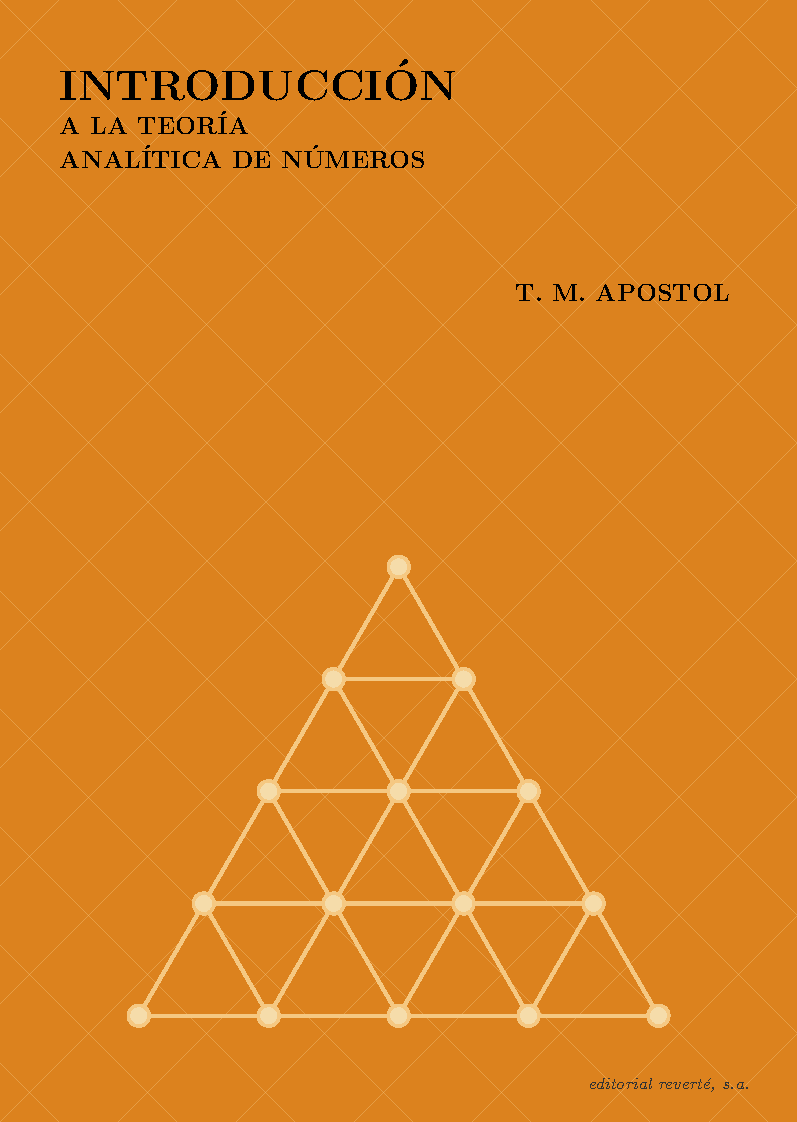
\includepdf[pages=1]{portada_apostol.pdf}

    \begin{titlepage}
    \centering
    \vspace*{3cm}

    {\fontsize{28}{36}\selectfont Introducción\\[6pt]
    a la Teoría\\[6pt]
    analítica de números\par}

    \vspace{2cm}

    {\fontsize{14}{18}\selectfont Tom M. Apostol\par}

    \vfill

    % Logo de Reverté (círculo aproximado si no tienes la imagen)
    % Si tienes el logo como imagen:
    % \includegraphics[width=2.5cm]{reverte_logo.png}
    \tikz\draw[thick] circle (1cm) node {\small\textbf{REVERTÉ}};

    \vspace{0.5cm}

    {\fontsize{11}{14}\selectfont\textbf{EDITORIAL REVERTÉ, S. A.}\par}

    \vspace{0.3cm}

    {\fontsize{8}{10}\selectfont
    Barcelona·Bogotá·Buenos Aires·Caracas·México·Rio de Janeiro\par}

    \vspace{1cm}
    \end{titlepage}

    \setcounter{page}{1}
    \tableofcontents

    \chapter{El teorema fundamental de la Aritmética}

    \section{INTRODUCCIÓN}

    En este capitulo se introducen conceptos básicos de la Teoría elemental de números tales
    como la divisibilidad, el máximo común divisor, y los números primos y compuestos. Los
    resultados principales son el teorema 1.2, que establece la existencia del máximo común
    divisor para todo par de enteros, y el teorema 1.10 (Teorema fundamental de la Aritmética),
    que demuestra que todo entero mayor que 1 se puede representar como prodcuto de factores
    primos de forma única (salvo el orden de los factores). Muchas de las demostraciones utilizan
    la sigueinte propiedad de enteros.

    \textbf{El principio de inducción}. Si $Q$ es un conjunto de enteros tales que
    \begin{enumerate}
        \item[(a)] $1\in Q$.
        \item[(b)] $n\in Q$ implica $n+1\in Q$, 
    \end{enumerate}
    entonces
    \begin{enumerate}
        \item[(c)] todo entero $\geq1$ pertenece a $Q$.
    \end{enumerate}

    Existen, además, otras formulaciones de este principio. Por ejemplo, en (a) podemos
    substituir 1 por un entero cualquiera $k$, siempre que en (c) la desigualdad $\geq1$
    se substituya por $\geq k$. Además (b) se puede substituir por $1,2,3,\dots,n\in Q$
    implica $(n+1)\in Q$.

    Suponemos que el lector se halla familiarizado con este principio así como con su uso en las
    demostraciones de teoremas por inducción. Le suponemos también familiarizado con el siguiente
    principio que es logicamente equivalente al principio de inducción.

    \textbf{El principio de buena ordenación.} Si $A$ es un conjunto no vacio de enteros positivos,
    entonces $A$ posee un elemento minimo.\\
    De nuevo, este principio posee formulaciones equivalentes. Por ejemplo, enteros positivos
    se puede substituir por enteros $\geq k$ para un cierto $k$.

    \section{DIVISIBILIDAD}

    \textbf{Notación.} En este capítulo, las letras latinas minúsculas $a,b,c,d,n,$ etc,
    denotan enteros; pueden ser positivos, negativos, o cero.

    \begin{definicion}[Divisibilidad]
        Diremos que $d$ divide $n$ y escribiremos $d\mid n$ si $n=cd$ para algun $c$.
        Diremos también que $n$ es múltiplo de $d$, que $d$ es un divisor de $n$, o que
        $d$ es un factor de $n$. Si $d$ no divide a $n$ escribiremos $d\nmid n$.
    \end{definicion}

    La divisibilidad establece una relación binaria entre enteros con las siguientes propiedades
    elementales cuyas demostraciones se dejan como ejercicio para el lector, (Salvo indicación
    expresa, las letras $a,b,d,m,n$ del teorema 1.1 representan enteros arbitrarios).

    \begin{teorema}
        La divisibilidad verifica las siguientes propiedades:
        \begin{enumerate}
            \item[(a)] $n\mid n$\hfill \textit{(propiedad reflexiva)}
            \item[(b)] $d\mid n$ y $n\mid m$ implica $d\mid m$\hfill\textit{(propiedad transitiva)}
            \item[(c)] $d\mid n$ y $d\mid m$ implica $d\mid(an+bm)$\hfill\textit{propiedad lineal}
            \item[(d)] $d\mid n$ implica $ad\mid an$\hfill\textit{(propiedad de multiplicación)}
            \item[(e)] $ad\mid an$ y $a\neq0$ implica $d\mid n$\hfill\textit{propiedad de simplificación}
            \item[(f)] $1\mid n$\hfill\textit{(1 divide a todos los enteros)}
            \item[(g)] $n\mid0$\hfill\textit{(cada entero divide a cero)}
            \item[(h)] $0\mid n$ implica $n=0$\hfill\textit{(el cero solo divide al cero)}
            \item[(i)] $d\mid n$ y $n\neq0$ implica $\abs{d}\leq\abs{n}$\hfill\textit{(propiedad de comparación)}
            \item[(j)] $d\mid n$ y $n\mid d$ implica $\abs{d}=\abs{n}$
            \item[(k)] $d\mid n$ y $d\neq0$ implica $(n/d)\mid n$
        \end{enumerate}
    \end{teorema}

    Nota. Si $d\mid n$ entonces $n/d$ se llama el divisor conjugado de $d$.

    \section{MÁXIMO COMÚN DIVISOR}

    Si un $d$ divide a dos enteros $a$ y $b$, entonces $d$ se llama \textit{divisor comun}
    de $a$ y $b$. Así, pues, 1 es un divisor común de todo par de enteros $a$ y $b$. Ahora
    demostraremos que todo par de enteros $a$ y $b$ poseen un divisor común que se puede expresar
    como combinación lineal de $a$ y $b$.

    \begin{teorema}
        Dados dos enteros $a$ y $b$, existe un divisor común de $a$ y $b$ de la forma
        \begin{equation*}
            d=ax+by,
        \end{equation*}
        en donde $x$ e $y$ son enteros. Además, todo divisor común de $a$ y $b$ divide a este
        $d$. 
    \end{teorema}

    \begin{proof}
        Ante todo suponemos que $a\geq0$ y $b\geq0$. Utilizamos inducción sobre $n$, en donde
        $n=a+b$. Si $n=0$ entonces $a=b=0$ y podemos tomar $d=0$ con $x=y=0$. Podemos pues suponer
        que el teorema se ha demostrado para $0,1,2,\dots,n-1$. Por simetria podemos suponer que
        $a\geq b$. Si $b=0$ tomamos $d=a$, $x=1$, $y=0$. Si $b\geq1$ aplicamos el teorema a
        $a-b$ y $b$. Puesto que un divisor común $d$ de $a-b$ y $b$ de la forma $d=(a-b)x+by$.
        Este $d$ divide también a $(a-b)+b=a$, luego $d$ es un divisor común de $a$ y $b$ y se
        tiene $d=ax+(y-x)b$, como combinación lineal de $a$ y $b$. Para completar la demostración
        necesitamos demostrar que cada divisor común divide a $d$. Pero un divisor común divide
        a $a$ y a $b$ y por lo tanto, por linealidad, divide a $d$. Si $a\lt0$ o $b\lt0$ (o ambos),
        podemos aplicar el resultado recién demostrado a $\abs{a}$ y $\abs{b}$. Entonces existe
        un divisor común  $d$ de $\abs{a}$ y $\abs{b}$ de la forma
        \begin{equation*}
            d=\abs{a}x+\abs{b}y.
        \end{equation*}
        Si $a\lt0$, $\abs{a}x=-ax=-a(-x)$. Análogamente, si $b\lt0$, $\abs{b}y=b(-y)$. Por
        lo tanto $d$ es también ahora combinación lineal de $a$ y $b$.
    \end{proof}

    \begin{teorema}
        Dados dos enteros $a$ y $b$, existe un número $d$ y sólo uno, con las siguiente
        propiedades:
        \begin{enumerate}
            \item[(a)] $d\geq0$\hfill\textit{($d$ es no negativo)}
            \item[(b)] $d\mid a$ y $d\mid b$\hfill\textit{($d$ es un divisor común de $a$ y de $b$)}
            \item[(c)] $e\mid a$ y $e\mid d$\hfill\textit{(cada divisor común divide a $d$)}  
        \end{enumerate}
    \end{teorema}

    \begin{proof}
        Por el teorema 1.2 por lo menos existe un $d$ que satisface las condiciones (b) y (c).
        Luego, $-d$ también las satisface. Pero si $d^{\prime}$ satisface (b) y (c), entonces
        $d\mid d^{\prime}$ y $d^{\prime}\mid d$, por lo tanto $\abs{d}=\abs{d^{\prime}}$. Luego
        existe exactamente un $d\geq0$ que satisface (b) y (c).
    \end{proof}
    
    Nota. En el teorema 1.3, $d=0$ si, y solo si, $a=b=0$ en cualquier otro caso $d\geq1.$

    \begin{definicion}[Máximo común divisor]
        El número $d$ del teorema 1.3 se llama \textbf{máximo cómun divisor (mcd)} de $a$ y
        $b$ se designa por $(a,b)$ o $aDb$. Si $(a,b)=1$ entonces se dice que $a$ y $b$ son
        primos entre si (o relativos).
    \end{definicion}

    La notación $aDb$ surge al interpretar el mcd como una operación entre $a$ y $b$. Sin
    embargo, la notación mas comunmente usada es $(a,b)$ y es la que adoptaremos, si bien
    en el proximo teorema utilizaremos también la notación $aDb$ con objeto de hacer resaltar
    las propiedades algebraicas de la operación $D$.
    
    \begin{teorema}
        El mcd posee las siguientes propiedades:
        \begin{enumerate}
            \item[(a)] $(a,b)=(b,a)$\hfill\textit{(ley conmutativa)}
            \item[(b)] $(a,(b,c))=((a,b),c)$\hfill\textit{(ley asociativa)}
            \item[(c)] $(ac,bc)=\abs{c}(a,b)$\hfill\textit{(ley distributiva)}
            \item[(d)] $(a,1)=(1,a)=1,\quad (a,0)=(0,a)=\abs{a}$.   
        \end{enumerate}
    \end{teorema}

    \begin{proof}
        Solamente demostraremos (c). Las otras demostraciones se dejan como ejercicio para el
        lector. Sea $d=(a,b)$ y sea $e=(ac,bc)$. Queremos demostrar que $e=\abs{c}d$. Escribimos
        $d=ax+by$. Entonces tenemos
        \begin{equation}
            cd=acx+bcy.
        \end{equation}
        Por lo tanto $cd\mid e$ puesto que $cd$ divide a $ac$ y $bc$. Además, la ecuación (1.1)
        prueba que $e\mid cd$ puesto que $e\mid ac$ y $e\mid bc$. Por lo tanto $\abs{e}=\abs{cd}$,
        o $e=\abs{c}d$.
    \end{proof}

    \begin{teorema}[Lema de Euclides]
        Si $a\mid bc$ y si $(a,b)=1$, entonces $a\mid c$.
    \end{teorema}

    \begin{proof}
        Puesto que $(a,b)=1$ podemos escribir $1=ax+by$. Por consiguiente $c=acx+bcy$. Pero
        $a\mid acx$ y $a\mid bcy$, luego $a\mid c$.
    \end{proof}

    \section{NÚMEROS PRIMOS}

    \begin{definicion}[Número primo]
        Un entero $n$ se llama primo si $n>1$ y si los únicos divisores positivos de $n$ son
        1 y $n$. Si $n>1$ y $n$ no es primo, entonces $n$ se llama compuesto.
    \end{definicion}

    \textbf{Ejemplos.} Los números primos menores que 100 son 2, 3, 5, 7, 11, 13, 17, 19, 23,
    29, 31, 37, 41, 43, 47, 53, 59, 61, 67, 71, 73, 79, 83, 89 y 97.

    \textbf{Notación.} Los números primos usualmente se designan por $p,p',p_i,q,q',q_i$.

    \begin{teorema}
        Cada entero $n>1$ o es primo o es producto de números primos.
    \end{teorema}

    \begin{proof}
        Utilizaremos inducción sobre $n$. El teorema es claro para $n=2$. Suponemos que es
        cierto para cada entero $<n$. Entonces si $n$ no es primo posee un divisor $d\neq1$,
        $d\neq n$. Por lo tanto $n=cd$, en donde $c\neq n$. Luego tanto $c$ como $d$ son $<n$
        y $>1$, por lo que cada uno de ellos es un producto de números primos, y entonces $n$
        también lo es.
    \end{proof}

    \begin{teorema}[Euclides]
        Existe una infinidad de números primos.
    \end{teorema}

    \begin{proof}
        Suponemos que sólo existe un número finito, por ejemplo $p_1,p_2,\dots,p_n$. Sea
        $N=1+p_1p_2\cdots p_n$. Puesto que $N>1$ o $N$ es primo o $N$ es un producto de
        primos. Pero $N$ no es primo ya que $N$ es mayor que cada uno de los $p_i$. Sin
        embargo ningún $p_i$ divide a $N$ (si $p_i\mid N$ entonces $p_i$ divide a la
        diferencia $N-p_1p_2\cdots p_n=1$). Lo que contradice el teorema 1.6.
    \end{proof}

    \begin{teorema}
        Si un primo $p$ no divide a $a$, entonces $(p,a)=1$.
    \end{teorema}

    \begin{proof}
        Sea $d=(p,a)$. Entonces $d\mid p$, luego o $d=1$ o $d=p$. Pero $d\mid a$ luego
        $d\neq p$ puesto que $p\nmid a$. En consecuencia $d=1$.
    \end{proof}

    \begin{teorema}
        Si un primo $p$ divide a $ab$, entonces $p\mid a$ ó $p\mid b$. En general, si un
        primo $p$ divide a un producto $a_1\cdots a_n$, entonces $p$ divide a uno, por lo
        menos, de los factores.
    \end{teorema}

    \begin{proof}
        Suponemos que $p\mid ab$ y que $p\nmid a$. Veremos que $p\mid b$. Por el teorema 1.8,
        $(p,a)=1$, luego por el lema de Euclides, $p\mid b$. Para demostrar la afirmación más
        general se emplea la inducción sobre $n$, número de factores. Los detalles se dejan
        al lector.
    \end{proof}

    \section{EL TEOREMA FUNDAMENTAL DE LA ARITMÉTICA}

    \begin{teorema}[Teorema fundamental de la Aritmética]
        Cada entero $n>1$ se puede representar como un producto de factores primos de forma
        única, salvo el orden de los factores.
    \end{teorema}

    \begin{proof}
        Usaremos la inducción sobre $n$. El teorema es verdadero para $n=2$. Suponemos,
        entonces, que es verdadero para todo entero mayor que 1 y menor que $n$. Probaremos
        que es verdadero también para $n$. Si $n$ es primo no hay que probar nada. Por lo
        tanto, suponemos que $n$ es compuesto y admite dos descomposiciones, que son
        \begin{equation*}
            n=p_1p_2\cdots p_s=q_1q_2\cdots q_t.
        \end{equation*}
        Queremos demostrar que $s=t$ y que cada $p$ es igual a algún $q$. Dado que $p_1$
        divide el producto $q_1q_2\cdots q_t$ debe dividir a uno, por lo menos, de los
        factores. Ordenaremos los $q_1,q_2,\dots,q_t$ de forma que $p_1\mid q_1$. Entonces
        $p_1=q_1$ ya que $p_1$ y $q_1$ son primos. En la descomposición anterior podemos
        dividir por $p_1$ obteniendo
        \begin{equation*}
            \frac{n}{p_1}=p_2\cdots p_s=q_2\cdots q_t.
        \end{equation*}
        Si $s>1$ o $t>1$, entonces $1<n/p_1<n$. La hipótesis de inducción nos dice que las
        dos descomposiciones de $n/p_1$ son idénticas, si prescindimos del orden de los
        factores. Por consiguiente $s=t$ y las descomposiciones anteriores son también
        idénticas, si prescindimos del orden de los factores. Esto completa la demostración.
    \end{proof}

    Nota. En la descomposición de un entero $n$, un cierto primo $p$ puede aparecer más de
    una vez. Si los factores primos distintos de $n$ son $p_1,\dots,p_r$ y si $p_i$ aparece
    $a_i$ veces como factor, escribiremos
    \begin{equation*}
        n=p_1^{a_1}\cdots p_r^{a_r},
    \end{equation*}
    o más brevemente,
    \begin{equation*}
        n=\prod_{i=1}^{r}p_i^{a_i}.
    \end{equation*}
    Esta expresión se llama descomposición de $n$ en factores primos. También es posible
    expresar el número 1 de esta forma tomando cada uno de los exponentes $a_i$ iguales a 0.

    \begin{teorema}
        Si $n=\prod_{i=1}^{r}p_i^{a_i}$, el conjunto de los divisores positivos de $n$ es el
        conjunto de los números de la forma $\prod_{i=1}^{r}p_i^{c_i}$, en donde
        $0\leq c_i\leq a_i$ para $i=1,2,\dots,r$.
    \end{teorema}

    \begin{proof}
        Ejercicio.
    \end{proof}

    Nota. Si escribimos los números primos en orden creciente, entonces
    \begin{equation*}
        p_1=2,\quad p_2=3,\quad p_3=5,\quad\dots,\quad p_n=\text{el $n$-ésimo primo},
    \end{equation*}
    cada entero positivo $n$ (incluido el 1) se puede expresar en la forma
    \begin{equation*}
        n=\prod_{i=1}^{\infty}p_i^{a_i}
    \end{equation*}
    en donde cada exponente $a_i\geq0$. Los divisores positivos de $n$ son todos los números
    de la forma
    \begin{equation*}
        \prod_{i=1}^{\infty}p_i^{c_i}
    \end{equation*}
    en donde $0\leq c_i\leq a_i$. Los productos son evidentemente finitos.

    \begin{teorema}
        Si dos enteros positivos $a$ y $b$ admiten las descomposiciones
        \begin{equation*}
            a=\prod_{i=1}^{\infty}p_i^{a_i},\qquad b=\prod_{i=1}^{\infty}p_i^{b_i},
        \end{equation*}
        su mcd admite la descomposición
        \begin{equation*}
            (a,b)=\prod_{i=1}^{\infty}p_i^{c_i}
        \end{equation*}
        en donde cada $c_i=\min\{a_i,b_i\}$, el menor de $a_i$ y $b_i$.
    \end{teorema}

    \begin{proof}
        Sea $d=\prod_{i=1}^{\infty}p_i^{c_i}$. Dado que $c_i\leq a_i$ y $c_i\leq b_i$ tenemos
        $d\mid a$ y $d\mid b$, luego $d$ es un divisor común de $a$ y $b$. Sea $e$ otro
        divisor común de $a$ y $b$, y consideremos la descomposición de
        $e=\prod_{i=1}^{\infty}p_i^{e_i}$. Entonces $e_i\leq a_i$ y $e_i\leq b_i$ o sea
        $e_i\leq c_i$. Por lo tanto $e\mid d$, luego $d$ es el mcd de $a$ y $b$.
    \end{proof}

    \section{LA SERIE DE LOS INVERSOS DE LOS PRIMOS}

    \begin{teorema}
        La serie infinita $\sum_{n=1}^{\infty}1/p_n$ diverge.
    \end{teorema}

    \begin{proof}
        La siguiente demostración de este teorema se debe a Clarkson. Suponemos que la serie
        converge y obtenemos una contradicción. Si la serie converge existe un entero $k$
        tal que
        \begin{equation*}
            \sum_{m=k+1}^{\infty}\frac{1}{p_m}<\frac{1}{2}.
        \end{equation*}
        Sea $Q=p_1\cdots p_k$, y consideremos los números $1+nQ$ para $n=1,2,\dots$. Ninguno
        de ellos es divisible por ninguno de los primos $p_1,\dots,p_k$. Por consiguiente,
        todos los factores primos de $1+nQ$ se hallan entre los primos $p_{k+1},p_{k+2},\dots$.
        Por consiguiente, para cada $r\geq1$ tenemos
        \begin{equation*}
            \sum_{n=1}^{r}\frac{1}{1+nQ}\leq\sum_{t=1}^{\infty}
            \left(\sum_{m=k+1}^{\infty}\frac{1}{p_m}\right)^{t},
        \end{equation*}
        puesto que la suma de la derecha contiene entre sus términos todos los términos de
        la izquierda. Pero el segundo miembro de esta desigualdad se halla dominado por la
        serie geométrica convergente
        \begin{equation*}
            \sum_{t=1}^{\infty}\left(\frac{1}{2}\right)^{t}.
        \end{equation*}
        Por consiguiente la serie $\sum_{n=1}^{\infty}1/(1+nQ)$ tiene sumas parciales
        acotadas y por lo tanto converge. Pero esto es contradictorio puesto que el criterio
        de la integral o el criterio de comparación del límite prueba que esta serie diverge.
    \end{proof}

    Nota. La divergencia de la serie $\sum1/p_n$ fue demostrada por primera vez en 1737 por
    Euler, que observó que implica el teorema de Euclides relativo a la existencia de una
    infinidad de primos. En un capítulo posterior obtendremos una fórmula asintótica que
    demuestra que las sumas parciales $\sum_{k=1}^{n}1/p_k$ tienden a infinito como
    $\log(\log n)$.

    \section{EL ALGORITMO DE EUCLIDES}

    El teorema 1.12 proporciona un método práctico para calcular el mcd $(a,b)$ cuando se
    conocen las descomposiciones en factores primos de $a$ y de $b$. Sin embargo, obtener
    estas descomposiciones en factores primos puede comportar considerables cálculos y es
    deseable disponer de un procedimiento que requiera menos esfuerzo. Existe un
    procedimiento útil conocido con el nombre de algoritmo de Euclides, que no requiere las
    descomposiciones de $a$ y $b$. Este procedimiento se basa en divisiones sucesivas y hace
    uso del teorema que sigue.

    \begin{teorema}[Algoritmo de división]
        Dados dos enteros $a$ y $b$ con $b>0$, existe un único par de enteros $q$ y $r$ tales
        que
        \begin{equation*}
            a=bq+r,\qquad\text{con } 0\leq r<b.
        \end{equation*}
        Además, $r=0$ si, y sólo si, $b\mid a$.
    \end{teorema}

    Nota. Se dice que $q$ es el cociente y $r$ el resto obtenido al dividir $a$ por $b$.

    \begin{proof}
        Sea $S$ el conjunto de enteros no negativos dado por
        \begin{equation*}
            S=\{y:y=a-bx,\ x\text{ es un entero},\ y\geq0\}.
        \end{equation*}
        Es un conjunto no vacío de enteros no negativos, por lo tanto admite mínimo, que
        designaremos $a-bq$. Sea $r=a-bq$. Entonces $a=bq+r$ y $r\geq0$. Ahora demostraremos
        que $r<b$. Supongamos $r\geq b$. Entonces $0\leq r-b<r$. Pero $r-b\in S$ ya que
        $r-b=a-b(q+1)$. Por lo tanto $r-b$ es un elemento de $S$ menor que su elemento
        mínimo $r$. Esta contradicción prueba que $r<b$. El par $q,r$ es único, ya que si
        existiese otro par con estas condiciones $q',r'$, entonces $bq+r=bq'+r'$, de donde
        $b(q-q')=r'-r$. Si $r'-r\neq0$ tendremos $b\leq\abs{r'-r}$, que constituye una
        contradicción. Por consiguiente $r'=r$ y $q'=q$. Finalmente es claro que $r=0$ si, y
        sólo si, $b\mid a$.
    \end{proof}

    Nota. A pesar de que el teorema 1.14 es un teorema de existencia, su demostración nos da
    un método para calcular el cociente $q$ y el resto $r$. Restamos de $a$ (o sumamos a $a$)
    múltiplos de $b$ hasta obtener el menor número no negativo de la forma $a-bx$.

    \begin{teorema}[Algoritmo de Euclides]
        Se dan dos enteros positivos $a$ y $b$, tales que $b\nmid a$. Se escribe $r_0=a$,
        $r_1=b$, y aplicamos repetidamente el algoritmo de división obteniendo un conjunto de
        restos $r_2,r_3,\dots,r_n,r_{n+1}$ definidos sucesivamente por las relaciones
        \begin{align*}
            r_0&=r_1q_1+r_2, & 0&<r_2<r_1,\\
            r_1&=r_2q_2+r_3, & 0&<r_3<r_2,\\
            &\ \vdots & &\\
            r_{n-2}&=r_{n-1}q_{n-1}+r_n, & 0&<r_n<r_{n-1},\\
            r_{n-1}&=r_nq_n+r_{n+1}, & r_{n+1}&=0.
        \end{align*}
        Entonces $r_n$, el último resto no nulo de este proceso, es $(a,b)$, el mcd de $a$ y
        $b$.
    \end{teorema}

    \begin{proof}
        Existe un momento en el que $r_{n+1}=0$ puesto que los $r_i$ son decrecientes y no
        negativos. La última relación, $r_{n-1}=r_nq_n$, demuestra que $r_n\mid r_{n-1}$. La
        anterior a la última prueba que $r_n\mid r_{n-2}$. Por inducción vemos que $r_n$
        divide a cada $r_i$. En particular $r_n\mid r_1=b$ y $r_n\mid r_0=a$, luego $r_n$ es
        un divisor común de $a$ y $b$. Ahora sea $d$ otro divisor común de $a$ y $b$. La
        definición de $r_2$ prueba que $d\mid r_2$. La relación que le sigue prueba que
        $d\mid r_3$. Por inducción, $d$ divide a cada $r_i$ luego $d\mid r_n$. Por lo tanto
        $r_n$ es el mcd requerido.
    \end{proof}

    \section{EL MÁXIMO COMÚN DIVISOR DE MÁS DE DOS NÚMEROS}

    El máximo común divisor de tres enteros $a,b,c$ se designa $(a,b,c)$ y se define por la
    relación
    \begin{equation*}
        (a,b,c)=(a,(b,c)).
    \end{equation*}
    Por el teorema 1.4(b) tenemos $(a,(b,c))=((a,b),c)$ luego el mcd depende únicamente de
    $a,b,c$ y no del orden en el que estén escritos.

    Análogamente, el mcd de $n$ enteros $a_1,\dots,a_n$ se define inductivamente por la
    relación
    \begin{equation*}
        (a_1,\dots,a_n)=(a_1,(a_2,\dots,a_n)).
    \end{equation*}
    De nuevo, este número es independiente del orden en que aparecen los $a_i$.

    Si $d=(a_1,\dots,a_n)$ es fácil comprobar que $d$ divide a cada uno de los $a_i$ y que
    cada divisor común divide a $d$. Además, $d$ es combinación lineal de los $a_i$. Es
    decir, existen enteros $x_1,\dots,x_n$ tales que
    \begin{equation*}
        (a_1,\dots,a_n)=a_1x_1+\cdots+a_nx_n.
    \end{equation*}

    Si $d=1$ los números se llaman primos entre sí. Por ejemplo 2, 3 y 10 son primos entre sí.

    Si $(a_i,a_j)=1$ siempre que $i\neq j$ se dice que los números $a_1,\dots,a_n$ son primos
    entre sí dos a dos. Si $a_1,\dots,a_n$ son primos entre sí dos a dos, entonces
    $(a_1,\dots,a_n)=1$. Sin embargo, el ejemplo $(2,3,10)$ muestra que el recíproco no es
    necesariamente verdadero.

    \section*{Ejercicios del capítulo 1}

    En estos ejercicios las letras latinas minúsculas $a,b,c,\dots,x,y,z$ representan
    enteros. Probar cada una de las afirmaciones de los ejercicios 1 al 6.

    \begin{ejercicio}
        Si $(a,b)=1$ y si $c\mid a$ y $d\mid b$, entonces $(c,d)=1$.
    \end{ejercicio}

    \begin{ejercicio}
        Si $(a,b)=(a,c)=1$, entonces $(a,bc)=1$.
    \end{ejercicio}

    \begin{ejercicio}
        Si $(a,b)=1$, entonces $(a^n,b^k)=1$ para todo $n\geq1$, $k\geq1$.
    \end{ejercicio}

    \begin{ejercicio}
        Si $(a,b)=1$, entonces $(a+b,a-b)$ o es 1 o es 2.
    \end{ejercicio}

    \begin{ejercicio}
        Si $(a,b)=1$, entonces $(a+b,a^2-ab+b^2)$ o es 1 o es 3.
    \end{ejercicio}

    \begin{ejercicio}
        Si $(a,b)=1$ y $d\mid(a+b)$, entonces $(a,d)=(b,d)=1$.
    \end{ejercicio}

    \begin{ejercicio}
        Un número racional $a/b$ con $(a,b)=1$ se llama \textit{fracción reducida}. Si la
        suma de dos fracciones reducidas es un entero, es decir, si $(a/b)+(c/d)=n$,
        demostrar que entonces $\abs{b}=\abs{d}$.
    \end{ejercicio}

    \begin{ejercicio}
        Un entero se llama \textit{sin cuadrados} si no es divisible por el cuadrado de
        ningún primo. Probar que, para cada $n\geq1$, existen $a>0$ y $b>0$, unívocamente
        determinados, tales que $n=a^2b$, en donde $b$ es sin cuadrados.
    \end{ejercicio}

    \begin{ejercicio}
        Para cada una de las afirmaciones que siguen, dar una demostración o un
        contraejemplo.
        \begin{enumerate}
            \item[(a)] Si $b^2\mid n$ y $a^2\mid n$ y $a^2\leq b^2$, entonces $a\mid b$.
            \item[(b)] Si $b^2$ es el mayor cuadrado que divide a $n$, entonces $a^2\mid n$
            implica $a\mid b$.
        \end{enumerate}
    \end{ejercicio}

    \begin{ejercicio}
        Dados $x$ e $y$, sean $m=ax+by$, $n=cx+dy$, en donde $ad-bc=\pm1$. Probar que
        $(m,n)=(x,y)$.
    \end{ejercicio}

    \begin{ejercicio}
        Probar que, si $n>1$, $n^4+4$ es compuesto.
    \end{ejercicio}

    En los ejercicios 12, 13 y 14, $a,b,c,m$ y $n$ designan enteros positivos.

    \begin{ejercicio}
        Establecer una demostración o un contraejemplo para cada una de las afirmaciones
        siguientes.
        \begin{enumerate}
            \item[(a)] Si $a^n\mid b^n$, entonces $a\mid b$.
            \item[(b)] Si $n^n\mid m^m$, entonces $n\mid m$.
            \item[(c)] Si $a^n\mid 2b^n$ y $n>1$, entonces $a\mid b$.
        \end{enumerate}
    \end{ejercicio}

    \begin{ejercicio}
        Si $(a,b)=1$ y $(a/b)^m=n$, probar que $b=1$. Si $n$ no es la potencia $m$-ésima de
        un entero positivo, entonces $n^{1/m}$ es irracional.
    \end{ejercicio}

    \begin{ejercicio}
        Si $(a,b)=1$ y $ab=c^n$, probar que $a=x^n$ y $b=y^n$ para algún $x$ y algún $y$.
        (Indicación: considerar $d=(a,c)$.)
    \end{ejercicio}

    \begin{ejercicio}
        Probar que cada $n\geq12$ es la suma de dos números compuestos.
    \end{ejercicio}

    \begin{ejercicio}
        Probar que, si $2^n-1$ es primo, entonces $n$ es primo.
    \end{ejercicio}

    \begin{ejercicio}
        Probar que, si $2^n+1$ es primo, entonces $n$ es una potencia de 2.
    \end{ejercicio}

    \begin{ejercicio}
        Si $m\neq n$ calcular el mcd $(a^{2^m}+1,a^{2^n}+1)$ en términos de $a$.
        (Indicación: Sea $A_n=a^{2^n}+1$ y probar que $A_n\mid(A_m-2)$ si $m>n$.)
    \end{ejercicio}

    \begin{ejercicio}
        La sucesión de Fibonacci $1,1,2,3,5,8,13,21,34,\dots$ se define por medio de la
        fórmula de recursión $a_{n+1}=a_n+a_{n-1}$, con $a_1=a_2=1$. Probar que, para cada
        $n$, $(a_n,a_{n+1})=1$.
    \end{ejercicio}

    \begin{ejercicio}
        Sea $d=(826,1890)$. Utilizar el algoritmo de Euclides para calcular $d$, y expresar
        entonces $d$ como combinación lineal de 826 y 1890.
    \end{ejercicio}

    \begin{ejercicio}
        El mínimo común múltiplo (mcm) de dos enteros $a$ y $b$ se designa por $[a,b]$ o por
        $aMb$, y se define como sigue:
        \begin{equation*}
            [a,b]=\abs{ab}/(a,b)\quad\text{si } a\neq0 \text{ y } b\neq0,
        \end{equation*}
        \begin{equation*}
            [a,b]=0\quad\text{si } a=0 \text{ o } b=0.
        \end{equation*}
        Probar que el mcm posee las siguientes propiedades:
        \begin{enumerate}
            \item[(a)] si $a=\prod_{i=1}^{r}p_i^{a_i}$ y $b=\prod_{i=1}^{r}p_i^{b_i}$ entonces
            $[a,b]=\prod_{i=1}^{r}p_i^{c_i}$, donde $c_i=\max\{a_i,b_i\}$.
            \item[(b)] $(aDb)Mc=(aMc)D(bMc)$.
            \item[(c)] $(aMb)Dc=(aDc)M(bDc)$.
        \end{enumerate}
        ($D$ y $M$ son distributivas una con respecto de la otra.)
    \end{ejercicio}

    \begin{ejercicio}
        Probar que $(a,b)=(a+b,[a,b])$.
    \end{ejercicio}

    \begin{ejercicio}
        La suma de dos enteros positivos es 5264 y su mínimo común múltiplo es 200340.
        Determinar ambos enteros.
    \end{ejercicio}

    \begin{ejercicio}
        Probar la siguiente propiedad multiplicativa del mcd:
        \begin{equation*}
            (ah,bk)=(a,b)(h,k)\left(\frac{a}{(a,b)},\frac{k}{(h,k)}\right)
            \left(\frac{b}{(a,b)},\frac{h}{(h,k)}\right).
        \end{equation*}
        En particular, si $(a,b)=(h,k)=1$, dicha propiedad prueba que $(ah,bk)=(a,k)(b,h)$.
    \end{ejercicio}

    Probar cada una de las afirmaciones de los ejercicios 25 al 28. Todos los enteros son
    positivos.

    \begin{ejercicio}
        Si $(a,b)=1$ existe un $x>0$ y un $y>0$ tales que $ax-by=1$.
    \end{ejercicio}

    \begin{ejercicio}
        Si $(a,b)=1$ y $x^a=y^b$ entonces $x=n^b$ e $y=n^a$ para un cierto $n$.
        (Indicación: Usar los ejercicios 25 y 13.)
    \end{ejercicio}

    \begin{ejercicio}
        \begin{enumerate}
            \item[(a)] Si $(a,b)=1$ entonces, para cada $n>ab$, existen positivos $x$ e $y$
            tales que $n=ax+by$.
            \item[(b)] Si $(a,b)=1$ no existen positivos $x$ e $y$ tales que $ab=ax+by$.
        \end{enumerate}
    \end{ejercicio}

    \begin{ejercicio}
        Si $a>1$, entonces $(a^m-1,a^n-1)=a^{(m,n)}-1$.
    \end{ejercicio}

    \begin{ejercicio}
        Dado $n>0$, sea $S$ un conjunto cuyos elementos sean enteros positivos $\leq2n$
        tales que, si $a$ y $b$ pertenecen a $S$ y $a\neq b$, entonces $a\nmid b$. ¿Cuál es
        el máximo número de enteros que puede contener $S$? (Indicación: $S$ puede contener,
        a lo sumo, uno de los enteros $1,2,2^2,2^3,\dots$, a lo sumo uno de los enteros
        $3,3\cdot2,3\cdot2^2,\dots$, etc.)
    \end{ejercicio}

    \begin{ejercicio}
        Si $n>1$ probar que la suma
        \begin{equation*}
            \sum_{k=1}^{n}\frac{1}{k}
        \end{equation*}
        no es un entero.
    \end{ejercicio}

\chapter{Funciones aritméticas y producto de Dirichlet}

    \section{INTRODUCCIÓN}

    La Teoría de números, como muchas otras partes de las Matemáticas, trata a menudo con
    sucesiones de números reales o complejos. En Teoría de números tales sucesiones se
    llaman \textit{funciones aritméticas}.

    \begin{definicion}[Función aritmética]
        Una función real —o compleja— definida sobre los enteros positivos se llama una
        función aritmética o una función de Teoría de números.
    \end{definicion}

    Este capítulo introduce varias funciones aritméticas que juegan un papel importante en
    el estudio de las propiedades de la divisibilidad de enteros y en la distribución de
    primos. El capítulo discute también la multiplicación de Dirichlet, un concepto que
    sirve para clarificar interrelaciones entre varias funciones aritméticas.

    Empezaremos con dos ejemplos importantes, la función de Möbius $\mu(n)$ y la función
    indicatriz de Euler $\varphi(n)$.

    \section{LA FUNCIÓN DE MÖBIUS $\mu(n)$}

    \begin{definicion}[Función de Möbius]
        La función de Möbius $\mu$ se define como sigue:
        \begin{equation*}
            \mu(1)=1;
        \end{equation*}
        si $n>1$, escribimos $n=p_1^{a_1}\cdots p_k^{a_k}$. Entonces
        \begin{align*}
            \mu(n)&=(-1)^k \quad\text{si } a_1=a_2=\cdots=a_k=1,\\
            \mu(n)&=0 \quad\text{en otro caso.}
        \end{align*}
    \end{definicion}

    Obsérvese que $\mu(n)=0$ si, y sólo si, $n$ admite un divisor cuadrado $>1$.

    He aquí una breve tabla de valores de $\mu(n)$:
    \begin{center}
        \begin{tabular}{c|cccccccccc}
            $n$: & 1 & 2 & 3 & 4 & 5 & 6 & 7 & 8 & 9 & 10\\
            \hline
            $\mu(n)$: & 1 & $-1$ & $-1$ & 0 & $-1$ & 1 & $-1$ & 0 & 0 & 1
        \end{tabular}
    \end{center}

    La función de Möbius interviene en diferentes lugares en Teoría de números. Una de sus
    principales propiedades es una fórmula simple, pero notable, relativa a la suma
    $\sum_{d\mid n}\mu(d)$, extendida sobre los divisores positivos de $n$. En esta fórmula
    $[x]$ designa el mayor entero $\leq x$.

    \begin{teorema}
        Si $n\geq1$ tenemos
        \begin{equation*}
            \sum_{d\mid n}\mu(d)=\left[\frac{1}{n}\right]=
            \begin{cases}
                1 & \text{si } n=1,\\
                0 & \text{si } n>1.
            \end{cases}
        \end{equation*}
    \end{teorema}

    \begin{proof}
        La fórmula es claramente cierta para $n=1$. Suponemos, entonces, que $n>1$ y
        escribimos $n=p_1^{a_1}\cdots p_k^{a_k}$. En la suma $\sum_{d\mid n}\mu(d)$ los
        únicos términos no nulos proceden de $d=1$ y de los divisores de $n$ que son
        productos de primos distintos. Entonces
        \begin{align*}
            \sum_{d\mid n}\mu(d)&=\mu(1)+\mu(p_1)+\cdots+\mu(p_k)+\mu(p_1p_2)+\cdots
            +\mu(p_{k-1}p_k)\\
            &\quad+\cdots+\mu(p_1p_2\cdots p_k)\\
            &=1+\binom{k}{1}(-1)+\binom{k}{2}(-1)^2+\cdots+\binom{k}{k}(-1)^k=(1-1)^k=0.
        \end{align*}
    \end{proof}

    \section{LA FUNCIÓN INDICATRIZ DE EULER $\varphi(n)$}

    \begin{definicion}[Indicatriz de Euler]
        Si $n\geq1$ la indicatriz de Euler $\varphi(n)$ es el número de enteros positivos
        menores que $n$ que son primos con $n$; así pues,
        \begin{equation*}
            \varphi(n)=\sideset{}{'}\sum_{k=1}^{n}1,
        \end{equation*}
        en donde la $'$ indica que la suma se halla extendida sobre los $k$ primos con $n$.
    \end{definicion}

    He aquí una breve tabla de valores de $\varphi(n)$:
    \begin{center}
        \begin{tabular}{c|cccccccccc}
            $n$: & 1 & 2 & 3 & 4 & 5 & 6 & 7 & 8 & 9 & 10\\
            \hline
            $\varphi(n)$: & 1 & 1 & 2 & 2 & 4 & 2 & 6 & 4 & 6 & 4
        \end{tabular}
    \end{center}

    Como en el caso de $\mu(n)$ existe una fórmula simple para la suma
    $\sum_{d\mid n}\varphi(d)$.

    \begin{teorema}
        Si $n\geq1$ tenemos
        \begin{equation*}
            \sum_{d\mid n}\varphi(d)=n.
        \end{equation*}
    \end{teorema}

    \begin{proof}
        Si $S$ designa el conjunto $\{1,2,\dots,n\}$, distribuimos los enteros de $S$ en
        conjuntos disjuntos de la forma siguiente. Para cada divisor $d$ de $n$, sea
        \begin{equation*}
            A(d)=\{k:(k,n)=d,\ 1\leq k\leq n\}.
        \end{equation*}
        Esto es, $A(d)$ contiene los elementos de $S$ cuyo mcd con $n$ es $d$. Los conjuntos
        $A(d)$ constituyen una partición de $S$. Por consiguiente, si $f(d)$ designa el
        número de enteros de $A(d)$, tenemos
        \begin{equation}
            \sum_{d\mid n}f(d)=n.
        \end{equation}
        Pero $(k,n)=d$ si, y sólo si, $(k/d,n/d)=1$, y $0<k\leq n$ si, y sólo si,
        $0<k/d\leq n/d$. Por consiguiente, si hacemos $q=k/d$, existe una correspondencia
        uno a uno entre los elementos de $A(d)$ y los enteros $q$ que satisfacen
        $0<q\leq n/d$, $(q,n/d)=1$. El número de tales $q$ es $\varphi(n/d)$. Por lo tanto
        $f(d)=\varphi(n/d)$ y (2) nos conduce a
        \begin{equation*}
            \sum_{d\mid n}\varphi(n/d)=n.
        \end{equation*}
        Pero esto es equivalente a la igualdad $\sum_{d\mid n}\varphi(d)=n$ puesto que $d$
        recorre todos los divisores de $n$ o sea los $n/d$. Y esto completa la demostración.
    \end{proof}

    \section{UNA RELACIÓN QUE CONECTA $\varphi$ Y $\mu$}

    La indicatriz de Euler está relacionada con la función de Möbius por medio de la
    fórmula que sigue:

    \begin{teorema}
        Si $n\geq1$ tenemos
        \begin{equation*}
            \varphi(n)=\sum_{d\mid n}\mu(d)\frac{n}{d}.
        \end{equation*}
    \end{teorema}

    \begin{proof}
        La suma que define $\varphi(n)$ se puede escribir en la forma
        \begin{equation*}
            \varphi(n)=\sum_{k=1}^{n}\left[\frac{1}{(n,k)}\right],
        \end{equation*}
        en donde $k$ recorre todos los enteros $\leq n$. Ahora utilizamos el teorema 2.1
        substituyendo $n$ por $(n,k)$ y obtenemos
        \begin{equation*}
            \varphi(n)=\sum_{k=1}^{n}\sum_{d\mid(n,k)}\mu(d)
            =\sum_{k=1}^{n}\sum_{\substack{d\mid n\\ d\mid k}}\mu(d).
        \end{equation*}
        Para un divisor $d$ de $n$ fijo podemos sumar respecto de todos los $k$ tales que
        $1\leq k\leq n$ que son múltiplos de $d$. Si escribimos $k=qd$ entonces
        $1\leq k\leq n$ si, y sólo si, $1\leq q\leq n/d$. Por lo tanto la última suma que da
        $\varphi(n)$ se puede escribir
        \begin{equation*}
            \varphi(n)=\sum_{d\mid n}\sum_{q=1}^{n/d}\mu(d)
            =\sum_{d\mid n}\mu(d)\sum_{q=1}^{n/d}1=\sum_{d\mid n}\mu(d)\frac{n}{d}.
        \end{equation*}
        Esto demuestra el teorema.
    \end{proof}

    \section{UNA FÓRMULA PRODUCTO PARA $\varphi(n)$}

    La suma que define $\varphi(n)$ en el teorema 2.3 se puede expresar también como un
    producto extendido a los divisores primos de $n$, distintos.

    \begin{teorema}
        Para $n\geq1$ tenemos
        \begin{equation}
            \varphi(n)=n\prod_{p\mid n}\left(1-\frac{1}{p}\right).
        \end{equation}
    \end{teorema}

    \begin{proof}
        Para $n=1$ el producto es vacío puesto que no existe ningún primo que divida a 1.
        En este caso entendemos que al producto se le asigna el valor 1.

        Suponemos, entonces, que $n>1$ y que $p_1,\dots,p_r$ son los divisores primos
        distintos de $n$. El producto se puede escribir
        \begin{align}
            \prod_{p\mid n}\left(1-\frac{1}{p}\right)&=\prod_{i=1}^{r}\left(1-\frac{1}{p_i}\right)\\
            &=1-\sum\frac{1}{p_i}+\sum\frac{1}{p_ip_j}-\sum\frac{1}{p_ip_jp_k}+\cdots
            +\frac{(-1)^r}{p_1p_2\cdots p_r}.
        \end{align}
        En el segundo miembro entendemos que en un término como $\sum1/p_ip_jp_k$ se
        consideran todos los posibles productos $p_ip_jp_k$ de factores primos distintos de
        $n$, tomando tres de ellos a un tiempo. Obsérvese que cada uno de los términos de la
        derecha de (4) es de la forma $\pm1/d$, en donde $d$ es un divisor de $n$ que es 1 o
        un producto de primos distintos. El numerador $\pm1$ es exactamente $\mu(d)$. Puesto
        que $\mu(d)=0$ si $d$ es divisible por el cuadrado de algún $p_i$ vemos que la suma
        de (4) es exactamente la misma que
        \begin{equation*}
            \sum_{d\mid n}\frac{\mu(d)}{d}.
        \end{equation*}
        Esto prueba el teorema.
    \end{proof}

    Muchas de las propiedades de $\varphi(n)$ se pueden deducir fácilmente de esta fórmula
    del producto. Se dan algunas de ellas en el siguiente teorema.

    \begin{teorema}
        La indicatriz de Euler posee las siguientes propiedades:
        \begin{enumerate}
            \item[(a)] $\varphi(p^\alpha)=p^\alpha-p^{\alpha-1}$ para $p$ primo y
            $\alpha\geq1$.
            \item[(b)] $\varphi(mn)=\varphi(m)\varphi(n)(d/\varphi(d))$, en donde $d=(m,n)$.
            \item[(c)] $\varphi(mn)=\varphi(m)\varphi(n)$ si $(m,n)=1$.
            \item[(d)] $a\mid b$ implica $\varphi(a)\mid\varphi(b)$.
            \item[(e)] $\varphi(n)$ es par para $n\geq3$. Además, si $n$ posee $r$ factores
            primos impares distintos, entonces $2^r\mid\varphi(n)$.
        \end{enumerate}
    \end{teorema}

    \begin{proof}
        La parte (a) se obtiene inmediatamente si en la fórmula del producto hacemos
        $n=p^\alpha$.

        Para probar (b) escribimos
        \begin{equation*}
            \frac{\varphi(n)}{n}=\prod_{p\mid n}\left(1-\frac{1}{p}\right).
        \end{equation*}
        Ahora observamos que cada divisor primo de $mn$ es un divisor primo de $m$ o de $n$,
        y aquellos divisores primos que dividen tanto a $m$ como a $n$ dividen también a
        $(m,n)$. Por lo tanto
        \begin{equation*}
            \frac{\varphi(mn)}{mn}=\prod_{p\mid mn}\left(1-\frac{1}{p}\right)
            =\frac{\displaystyle\prod_{p\mid m}\left(1-\frac{1}{p}\right)
            \prod_{p\mid n}\left(1-\frac{1}{p}\right)}{\displaystyle\prod_{p\mid(m,n)}
            \left(1-\frac{1}{p}\right)}
            =\frac{\dfrac{\varphi(m)}{m}\dfrac{\varphi(n)}{n}}{\dfrac{\varphi(d)}{d}},
        \end{equation*}
        por lo que obtenemos (b). La parte (c) es un caso especial de la parte (b).

        Ahora deducimos (d) de (b). Dado que $a\mid b$ tenemos $b=ac$ en donde
        $1\leq c\leq b$. Si $c=b$, entonces $a=1$ y la parte (d) se verifica trivialmente.
        Por consiguiente, suponemos que $c<b$. De (b) tenemos
        \begin{equation}
            \varphi(b)=\varphi(ac)=\varphi(a)\varphi(c)\frac{d}{\varphi(d)}
            =d\varphi(a)\frac{\varphi(c)}{\varphi(d)},
        \end{equation}
        en donde $d=(a,c)$. Ahora el resultado se obtiene por inducción sobre $b$. Para
        $b=1$ se sigue trivialmente. Suponemos, pues, que (5) se verifica para todo entero
        $<b$. Entonces se verifica para $c$ luego, puesto que $d\mid c$, $\varphi(d)\mid
        \varphi(c)$. Por lo que el segundo miembro de (5) es un múltiplo de $\varphi(a)$, es
        decir, $\varphi(a)\mid\varphi(b)$. Esto prueba (d).

        Ahora demostraremos (e). Si $n=2^\alpha$, $\alpha\geq2$, la parte (a) prueba que
        $\varphi(n)$ es par. Si $n$ posee, por lo menos, un divisor primo impar escribimos
        \begin{equation*}
            \varphi(n)=n\prod_{p\mid n}\frac{p-1}{p}
            =\frac{n}{\displaystyle\prod_{p\mid n}p}\prod_{p\mid n}(p-1)=c(n)\prod_{p\mid n}(p-1),
        \end{equation*}
        en donde $c(n)$ es un entero. El producto que multiplica a $c(n)$ es par así que
        $\varphi(n)$ es par. Además, cada primo impar $p$ proporciona un factor 2 a este
        producto, por lo tanto $2^r\mid\varphi(n)$ si $n$ tiene $r$ factores primos impares
        distintos.
    \end{proof}

    \section{EL PRODUCTO DE DIRICHLET DE FUNCIONES ARITMÉTICAS}

    En el teorema 2.3 hemos probado que
    \begin{equation*}
        \varphi(n)=\sum_{d\mid n}\mu(d)\frac{n}{d}.
    \end{equation*}
    La suma del segundo miembro es de un tipo que interviene frecuentemente en Teoría de
    números. Estas sumas tienen la forma
    \begin{equation*}
        \sum_{d\mid n}f(d)g\left(\frac{n}{d}\right)
    \end{equation*}
    en donde $f$ y $g$ son funciones aritméticas, y merece la pena estudiar algunas
    propiedades que estas sumas tienen en común. Veremos más adelante que las sumas de este
    tipo aparecen de forma natural en la teoría de las series de Dirichlet. Resulta de
    utilidad tratar estas sumas como un nuevo tipo de multiplicación de funciones
    aritméticas, punto de vista introducido por E. T. Bell en 1915.

    \begin{definicion}[Producto de Dirichlet]
        Si $f$ y $g$ son dos funciones aritméticas definimos su producto de Dirichlet (o
        convolución de Dirichlet) como la función aritmética $h$ definida por
        \begin{equation*}
            h(n)=\sum_{d\mid n}f(d)g\left(\frac{n}{d}\right).
        \end{equation*}
    \end{definicion}

    \textbf{Notación.} Escribiremos $f*g$ en vez de $h$ y $(f*g)(n)$ en vez de $h(n)$. El
    símbolo $N$ se utilizará para la función aritmética tal que $N(n)=n$ para todo $n$. Con
    esta notación, el teorema 2.3 se puede establecer en la forma
    \begin{equation*}
        \varphi=\mu*N.
    \end{equation*}

    El teorema que sigue describe propiedades algebraicas de la multiplicación de
    Dirichlet.

    \begin{teorema}
        La multiplicación de Dirichlet es asociativa y conmutativa. Esto es, para toda
        terna de funciones aritméticas $f,g,k$, tenemos
        \begin{align*}
            f*g&=g*f &&\text{(ley conmutativa)}\\
            (f*g)*k&=f*(g*k) &&\text{(ley asociativa).}
        \end{align*}
    \end{teorema}

    \begin{proof}
        Observemos ante todo que la definición de $f*g$ se puede expresar como sigue
        \begin{equation*}
            (f*g)(n)=\sum_{a\cdot b=n}f(a)g(b),
        \end{equation*}
        en donde $a$ y $b$ varían sobre el conjunto de todos los enteros positivos cuyo
        producto es $n$. Esto hace evidente la propiedad conmutativa.

        Para probar la propiedad asociativa sea $A=g*k$ y consideremos $f*A=f*(g*k)$.
        Tenemos
        \begin{align*}
            (f*A)(n)&=\sum_{a\cdot d=n}f(a)A(d)=\sum_{a\cdot d=n}f(a)\sum_{b\cdot c=d}g(b)k(c)\\
            &=\sum_{a\cdot b\cdot c=n}f(a)g(b)k(c).
        \end{align*}
        De la misma forma, si $B=f*g$ y consideramos $B*k$ obtenemos la misma fórmula para
        $(B*k)(n)$. Por lo tanto $f*A=B*k$ lo que indica que la multiplicación de Dirichlet
        es asociativa.
    \end{proof}

    Ahora introducimos un elemento identidad para esta multiplicación.

    \begin{definicion}[Función identidad]
        La función aritmética $I$ dada por
        \begin{equation*}
            I(n)=\left[\frac{1}{n}\right]=
            \begin{cases}
                1 & \text{si } n=1,\\
                0 & \text{si } n>1,
            \end{cases}
        \end{equation*}
        se llama la función identidad.
    \end{definicion}

    \begin{teorema}
        Para todo $f$ se tiene $I*f=f*I=f$.
    \end{teorema}

    \begin{proof}
        Tenemos
        \begin{equation*}
            (f*I)(n)=\sum_{d\mid n}f(d)I\left(\frac{n}{d}\right)
            =\sum_{d\mid n}f(d)\left[\frac{d}{n}\right]=f(n)
        \end{equation*}
        ya que $[d/n]=0$ si $d<n$.
    \end{proof}

    \section{INVERSOS DE DIRICHLET Y FÓRMULA DE INVERSIÓN DE MÖBIUS}

    \begin{teorema}
        Si $f$ es una función aritmética con $f(1)\neq0$ existe una única función
        aritmética $f^{-1}$, llamada inversa de Dirichlet de $f$, tal que
        \begin{equation*}
            f*f^{-1}=f^{-1}*f=I.
        \end{equation*}
        Además, $f^{-1}$ se obtiene por medio de las fórmulas de recurrencia
        \begin{equation*}
            f^{-1}(1)=\frac{1}{f(1)},\qquad
            f^{-1}(n)=\frac{-1}{f(1)}\sum_{\substack{d\mid n\\ d<n}}
            f\left(\frac{n}{d}\right)f^{-1}(d)\quad\text{para } n>1.
        \end{equation*}
    \end{teorema}

    \begin{proof}
        Dada $f$, veremos que la ecuación $(f*f^{-1})(n)=I(n)$ tiene una solución única
        dada por los valores de la función $f^{-1}(n)$. Para $n=1$ debemos resolver la
        ecuación
        \begin{equation*}
            (f*f^{-1})(1)=I(1)
        \end{equation*}
        que se reduce a
        \begin{equation*}
            f(1)f^{-1}(1)=1.
        \end{equation*}
        Puesto que $f(1)\neq0$ existe una solución y sólo una, que es $f^{-1}(1)=1/f(1)$.
        Ahora suponemos que los valores funcionales $f^{-1}(k)$ se han determinado de forma
        única para todo $k<n$. Entonces debemos resolver la ecuación $(f*f^{-1})(n)=I(n)$,
        o bien
        \begin{equation*}
            \sum_{d\mid n}f\left(\frac{n}{d}\right)f^{-1}(d)=0.
        \end{equation*}
        Podemos escribirla en la forma
        \begin{equation*}
            f(1)f^{-1}(n)+\sum_{\substack{d\mid n\\ d<n}}f\left(\frac{n}{d}\right)f^{-1}(d)=0.
        \end{equation*}
        Si conocemos los valores $f^{-1}(d)$ para todo divisor $d<n$, existe un valor
        unívocamente determinado para $f^{-1}(n)$, a saber,
        \begin{equation*}
            f^{-1}(n)=\frac{-1}{f(1)}\sum_{\substack{d\mid n\\ d<n}}
            f\left(\frac{n}{d}\right)f^{-1}(d),
        \end{equation*}
        puesto que $f(1)\neq0$. Esto establece la existencia y unicidad de $f^{-1}$ por
        inducción.
    \end{proof}

    Nota. Tenemos $(f*g)(1)=f(1)g(1)$. Luego, si $f(1)\neq0$ y $g(1)\neq0$, entonces
    $(f*g)(1)\neq0$. Este hecho, junto con los teoremas 2.6, 2.7 y 2.8, nos dice que, en el
    lenguaje de la teoría de grupos, el conjunto de todas las funciones aritméticas $f$ con
    $f(1)\neq0$ constituye un grupo abeliano con respecto de la operación $*$, siendo el
    elemento neutro la función $I$. El lector puede verificar con facilidad que
    \begin{equation*}
        (f*g)^{-1}=f^{-1}*g^{-1}\quad\text{si } f(1)\neq0 \text{ y } g(1)\neq0.
    \end{equation*}

    \begin{definicion}[Función unidad]
        Definimos la función unidad $u$ como la función aritmética tal que $u(n)=1$ para
        todo $n$.
    \end{definicion}

    El teorema 2.1 establece que $\sum_{d\mid n}\mu(d)=I(n)$. Con la notación de la
    multiplicación de Dirichlet se expresa
    \begin{equation*}
        \mu*u=I.
    \end{equation*}
    Entonces $u$ y $\mu$ son inversas de Dirichlet una de otra:
    \begin{equation*}
        u=\mu^{-1}\qquad\text{y}\qquad \mu=u^{-1}.
    \end{equation*}

    Esta propiedad simple de la función de Möbius, junto con la asociatividad de la
    multiplicación de Dirichlet, nos permite establecer una demostración simple del teorema
    que sigue.

    \begin{teorema}[Fórmula de inversión de Möbius]
        La ecuación
        \begin{equation}
            f(n)=\sum_{d\mid n}g(d)
        \end{equation}
        implica
        \begin{equation}
            g(n)=\sum_{d\mid n}f(d)\mu\left(\frac{n}{d}\right).
        \end{equation}
        Recíprocamente, (7) implica (6).
    \end{teorema}

    \begin{proof}
        La ecuación (6) establece que $f=g*u$. Multiplicando por $\mu$ obtenemos
        $f*\mu=(g*u)*\mu=g*(u*\mu)=g*I=g$, que es (7). Recíprocamente, la multiplicación de
        $f*\mu=g$ por $u$ nos da (6).
    \end{proof}

    La fórmula de inversión de Möbius ha sido ilustrada ya por el par de fórmulas de los
    teoremas 2.2 y 2.3:
    \begin{equation*}
        n=\sum_{d\mid n}\varphi(d),\qquad \varphi(n)=\sum_{d\mid n}d\mu\left(\frac{n}{d}\right).
    \end{equation*}

    \section{LA FUNCIÓN DE MANGOLDT $\Lambda(n)$}

    Ahora introducimos la función de Mangoldt $\Lambda$ que juega un papel central en la
    distribución de primos.

    \begin{definicion}[Función de Mangoldt]
        Para cada entero $n\geq1$ definimos
        \begin{equation*}
            \Lambda(n)=
            \begin{cases}
                \log p & \text{si } n=p^m \text{ para un cierto primo } p \text{ y un cierto } m\geq1,\\
                0 & \text{en otro caso.}
            \end{cases}
        \end{equation*}
    \end{definicion}

    He aquí una tabla breve de valores de $\Lambda(n)$:
    \begin{center}
        \begin{tabular}{c|cccccccccc}
            $n$: & 1 & 2 & 3 & 4 & 5 & 6 & 7 & 8 & 9 & 10\\
            \hline
            $\Lambda(n)$: & 0 & $\log2$ & $\log3$ & $\log2$ & $\log5$ & 0 & $\log7$ &
            $\log2$ & $\log3$ & 0
        \end{tabular}
    \end{center}

    La demostración del teorema que sigue muestra cómo esta función surge naturalmente del
    teorema fundamental de la Aritmética.

    \begin{teorema}
        Si $n\geq1$ tenemos
        \begin{equation}
            \log n=\sum_{d\mid n}\Lambda(d).
        \end{equation}
    \end{teorema}

    \begin{proof}
        El teorema es cierto para $n=1$ ya que ambos miembros son 0. Por consiguiente,
        suponemos que $n>1$ y escribimos
        \begin{equation*}
            n=\prod_{k=1}^{r}p_k^{a_k}.
        \end{equation*}
        Tomando logaritmos tenemos
        \begin{equation*}
            \log n=\sum_{k=1}^{r}a_k\log p_k.
        \end{equation*}
        Ahora consideramos la suma del segundo miembro de (8). Los únicos términos no nulos
        de la suma provienen de los divisores $d$ de la forma $p_k^m$ para
        $m=1,2,\dots,a_k$ y $k=1,2,\dots,r$. Luego
        \begin{equation*}
            \sum_{d\mid n}\Lambda(d)=\sum_{k=1}^{r}\sum_{m=1}^{a_k}\Lambda(p_k^m)
            =\sum_{k=1}^{r}\sum_{m=1}^{a_k}\log p_k=\sum_{k=1}^{r}a_k\log p_k=\log n,
        \end{equation*}
        que prueba (8).
    \end{proof}

    Ahora utilizamos la inversión de Möbius para expresar $\Lambda(n)$ en términos del
    logaritmo.

    \begin{teorema}
        Si $n\geq1$ tenemos
        \begin{equation*}
            \Lambda(n)=\sum_{d\mid n}\mu(d)\log\frac{n}{d}=-\sum_{d\mid n}\mu(d)\log d.
        \end{equation*}
    \end{teorema}

    \begin{proof}
        Invirtiendo (8) por la fórmula de inversión de Möbius obtenemos
        \begin{align*}
            \Lambda(n)&=\sum_{d\mid n}\mu(d)\log\frac{n}{d}
            =\log n\sum_{d\mid n}\mu(d)-\sum_{d\mid n}\mu(d)\log d\\
            &=I(n)\log n-\sum_{d\mid n}\mu(d)\log d.
        \end{align*}
        Puesto que $I(n)\log n=0$ para todo $n$, la demostración queda establecida.
    \end{proof}

    \section{FUNCIONES MULTIPLICATIVAS}

    Hemos observado ya que el conjunto de todas las funciones aritméticas $f$ con
    $f(1)\neq0$ forma un grupo abeliano respecto de la multiplicación de Dirichlet. En esta
    sección discutimos un subgrupo de este importante grupo, llamado de las funciones
    \textit{multiplicativas}.

    \begin{definicion}[Función multiplicativa]
        Una función aritmética $f$ se llama función multiplicativa si $f$ no es
        idénticamente nula y si
        \begin{equation*}
            f(mn)=f(m)f(n)\quad\text{siempre que } (m,n)=1.
        \end{equation*}
        Una función multiplicativa $f$ se llama completamente multiplicativa si verifica
        \begin{equation*}
            f(mn)=f(m)f(n)\quad\text{para todo } m,n.
        \end{equation*}
    \end{definicion}

    \begin{ejemplo}
        Sea $f_\alpha(n)=n^\alpha$, en donde $\alpha$ es un número real o complejo fijo.
        Esta función es completamente multiplicativa. En particular, la función unidad
        $u=f_0$ es completamente multiplicativa. La función $f_\alpha$ la designaremos por
        $N^\alpha$ y la llamaremos función potencia.
    \end{ejemplo}

    \begin{ejemplo}
        La función identidad $I(n)=[1/n]$ es completamente multiplicativa.
    \end{ejemplo}

    \begin{ejemplo}
        La función de Möbius es multiplicativa pero no es completamente multiplicativa. Es
        fácil verlo a partir de la definición de $\mu(n)$. Consideremos dos primos
        relativos $m$ y $n$. Si $m$ o $n$ posee un divisor que es cuadrado de un primo
        también lo posee $mn$, y tanto $\mu(mn)$ como $\mu(m)\mu(n)$ son cero. Si ninguno de
        ellos contiene un divisor cuadrático, entonces $m=p_1\cdots p_s$ y $n=q_1\cdots q_t$
        en donde los $p_i$ y los $q_i$ son primos distintos. Luego $\mu(m)=(-1)^s$,
        $\mu(n)=(-1)^t$ y $\mu(mn)=(-1)^{s+t}=\mu(m)\mu(n)$. Ello demuestra que $\mu$ es
        multiplicativa. No es completamente multiplicativa puesto que $\mu(4)=0$ y, en
        cambio, $\mu(2)\mu(2)=1$.
    \end{ejemplo}

    \begin{ejemplo}
        La indicatriz de Euler $\varphi(n)$ es multiplicativa. Esta es la parte (c) del
        teorema 2.5. No es completamente multiplicativa puesto que $\varphi(4)=2$ mientras
        que $\varphi(2)\varphi(2)=1$.
    \end{ejemplo}

    \begin{ejemplo}
        El producto ordinario $fg$ de dos funciones aritméticas $f$ y $g$ se define por
        medio de la fórmula usual
        \begin{equation*}
            (fg)(n)=f(n)g(n).
        \end{equation*}
        Análogamente, el cociente $f/g$ se define por medio de la fórmula
        \begin{equation*}
            \left(\frac{f}{g}\right)(n)=\frac{f(n)}{g(n)}\quad\text{siempre que } g(n)\neq0.
        \end{equation*}
        Si $f$ y $g$ son multiplicativas, $fg$ y $f/g$ también lo son. Si $f$ y $g$ son
        completamente multiplicativas, también lo son $fg$ y $f/g$.
    \end{ejemplo}

    Deducimos ahora algunas propiedades comunes a todas las funciones multiplicativas.

    \begin{teorema}
        Si $f$ es multiplicativa, entonces $f(1)=1$.
    \end{teorema}

    \begin{proof}
        Tenemos $f(n)=f(1)f(n)$ puesto que $(n,1)=1$ para todo $n$. Dado que $f$ no es
        idénticamente nula tenemos $f(n)\neq0$ para algún $n$, luego $f(1)=1$.
    \end{proof}

    Nota. Puesto que $\Lambda(1)=0$, la función de Mangoldt no es multiplicativa.

    \begin{teorema}
        Dada $f$ con $f(1)=1$, entonces:
        \begin{enumerate}
            \item[(a)] $f$ es multiplicativa si, y sólo si,
            \begin{equation*}
                f(p_1^{a_1}\cdots p_r^{a_r})=f(p_1^{a_1})\cdots f(p_r^{a_r})
            \end{equation*}
            para todos los primos $p_i$ y todos los enteros $a_i\geq1$.
            \item[(b)] Si $f$ es multiplicativa, entonces $f$ es completamente
            multiplicativa si, y sólo si,
            \begin{equation*}
                f(p^a)=f(p)^a
            \end{equation*}
            para todos los primos $p$ y todos los enteros $a\geq1$.
        \end{enumerate}
    \end{teorema}

    \begin{proof}
        La demostración se deduce fácilmente de las definiciones y se deja como ejercicio
        al lector.
    \end{proof}

    \section{FUNCIONES MULTIPLICATIVAS Y PRODUCTO DE DIRICHLET}

    \begin{teorema}
        Si $f$ y $g$ son multiplicativas, también lo es su producto de Dirichlet $f*g$.
    \end{teorema}

    \begin{proof}
        Sea $h=f*g$ y elijamos dos enteros primos entre sí $m$ y $n$. Entonces
        \begin{equation*}
            h(mn)=\sum_{c\mid mn}f(c)g\left(\frac{mn}{c}\right).
        \end{equation*}
        Ahora bien cada divisor $c$ de $mn$ se puede expresar en la forma $c=ab$ en donde
        $a\mid m$ y $b\mid n$. Además, $(a,b)=1$, $(m/a,n/b)=1$, y existe una
        correspondencia uno a uno entre el conjunto de los productos $ab$ y el de los
        divisores $c$ de $mn$. Por lo tanto
        \begin{align*}
            h(mn)&=\sum_{\substack{a\mid m\\ b\mid n}}f(ab)g\left(\frac{mn}{ab}\right)
            =\sum_{\substack{a\mid m\\ b\mid n}}f(a)f(b)g\left(\frac{m}{a}\right)g\left(\frac{n}{b}\right)\\
            &=\sum_{a\mid m}f(a)g\left(\frac{m}{a}\right)\sum_{b\mid n}f(b)g\left(\frac{n}{b}\right)=h(m)h(n).
        \end{align*}
        Esto termina la demostración.
    \end{proof}

    Advertencia. El producto de Dirichlet de dos funciones completamente multiplicativas
    no es necesariamente completamente multiplicativo.

    Una ligera modificación en la demostración precedente nos permite probar:

    \begin{teorema}
        Si $g$ y $f*g$ son multiplicativas, $f$ también es multiplicativa.
    \end{teorema}

    \begin{proof}
        Supondremos que $f$ no es multiplicativa y deduciremos que $f*g$ tampoco lo es.
        Sea $h=f*g$. Dado que $f$ no es multiplicativa existen enteros positivos $m$ y $n$
        con $(m,n)=1$ tales que
        \begin{equation*}
            f(mn)\neq f(m)f(n).
        \end{equation*}
        Elegimos el par $m,n$ de forma que el producto $mn$ sea mínimo.

        Si $mn=1$ entonces $f(1)\neq f(1)f(1)$ luego $f(1)\neq1$. Por lo tanto
        $h(1)=f(1)g(1)=f(1)\neq1$, que demuestra que $h$ no es multiplicativa.

        Si $mn>1$, entonces tenemos $f(ab)=f(a)f(b)$ para todo par de enteros positivos $a$
        y $b$ con $(a,b)=1$ y $ab<mn$. Ahora argüimos como en la demostración del teorema
        2.14, con la excepción de que en la suma que define $h(mn)$ separamos los términos
        que corresponden a $a=m$, $b=n$. Entonces tenemos
        \begin{align*}
            h(mn)&=\sum_{\substack{a\mid m\\ b\mid n\\ ab<mn}}f(ab)g\left(\frac{mn}{ab}\right)
            +f(mn)g(1)
            =\sum_{\substack{a\mid m\\ b\mid n\\ ab<mn}}f(a)f(b)g\left(\frac{m}{a}\right)g\left(\frac{n}{b}\right)+f(mn)\\
            &=\sum_{a\mid m}f(a)g\left(\frac{m}{a}\right)\sum_{b\mid n}f(b)g\left(\frac{n}{b}\right)-f(m)f(n)+f(mn)\\
            &=h(m)h(n)-f(m)f(n)+f(mn).
        \end{align*}
        Puesto que $f(mn)\neq f(m)f(n)$ esto demuestra que $h(mn)\neq h(m)h(n)$, luego $h$
        no es multiplicativa. Esta contradicción termina la demostración.
    \end{proof}

    \begin{teorema}
        Si $g$ es multiplicativa, también lo es su inversa de Dirichlet $g^{-1}$.
    \end{teorema}

    \begin{proof}
        Se deduce inmediatamente del teorema 2.15 ya que $g$ y $g*g^{-1}=I$ son ambas
        multiplicativas. (Ver ejercicio 34 para otra demostración.)
    \end{proof}

    Nota. Los teoremas 2.14 y 2.16 demuestran que el conjunto de las funciones
    multiplicativas constituye un subgrupo del grupo de todas las funciones aritméticas $f$
    con $f(1)\neq0$.

    \section{LA INVERSA DE UNA FUNCIÓN COMPLETAMENTE MULTIPLICATIVA}

    La inversa de Dirichlet de una función completamente multiplicativa es
    particularmente fácil de calcular.

    \begin{teorema}
        Sea $f$ multiplicativa. Entonces $f$ es completamente multiplicativa si, y sólo
        si,
        \begin{equation*}
            f^{-1}(n)=\mu(n)f(n)\quad\text{para todo } n\geq1.
        \end{equation*}
    \end{teorema}

    \begin{proof}
        Sea $g(n)=\mu(n)f(n)$. Si $f$ es completamente multiplicativa tenemos
        \begin{equation*}
            (g*f)(n)=\sum_{d\mid n}\mu(d)f(d)f\left(\frac{n}{d}\right)
            =f(n)\sum_{d\mid n}\mu(d)=f(n)I(n)=I(n)
        \end{equation*}
        puesto que $f(1)=1$ e $I(n)=0$ para $n>1$. Luego $g=f^{-1}$.

        Recíprocamente, suponemos $f^{-1}(n)=\mu(n)f(n)$. Para probar que $f$ es
        completamente multiplicativa basta demostrar que $f(p^a)=f(p)^a$ para potencias de
        primos. La ecuación $f^{-1}(n)=\mu(n)f(n)$ implica que
        \begin{equation*}
            \sum_{d\mid n}\mu(d)f(d)f\left(\frac{n}{d}\right)=0\qquad\text{para todo } n>1.
        \end{equation*}
        Luego, si tomamos $n=p^a$, tenemos
        \begin{equation*}
            \mu(1)f(1)f(p^a)+\mu(p)f(p)f(p^{a-1})=0,
        \end{equation*}
        de lo que obtenemos $f(p^a)=f(p)f(p^{a-1})$. Ello implica $f(p^a)=f(p)^a$, luego $f$
        es completamente multiplicativa.
    \end{proof}

    \begin{ejemplo}
        \textit{La inversa de la función $\varphi$ de Euler.} Puesto que $\varphi=\mu*N$
        tenemos $\varphi^{-1}=\mu^{-1}*N^{-1}$. Pero $N^{-1}=\mu N$ puesto que $N$ es
        completamente multiplicativa, luego
        \begin{equation*}
            \varphi^{-1}=\mu^{-1}*\mu N=u*\mu N.
        \end{equation*}
        Por lo tanto
        \begin{equation*}
            \varphi^{-1}(n)=\sum_{d\mid n}d\mu(d).
        \end{equation*}
        El teorema que sigue demuestra que
        \begin{equation*}
            \varphi^{-1}(n)=\prod_{p\mid n}(1-p).
        \end{equation*}
    \end{ejemplo}

    \begin{teorema}
        Si $f$ es multiplicativa tenemos
        \begin{equation*}
            \sum_{d\mid n}\mu(d)f(d)=\prod_{p\mid n}(1-f(p)).
        \end{equation*}
    \end{teorema}

    \begin{proof}
        Sea
        \begin{equation*}
            g(n)=\sum_{d\mid n}\mu(d)f(d).
        \end{equation*}
        Entonces $g$ es multiplicativa, luego para determinar $g(n)$ es suficiente calcular
        $g(p^a)$. Pero
        \begin{equation*}
            g(p^a)=\sum_{d\mid p^a}\mu(d)f(d)=\mu(1)f(1)+\mu(p)f(p)=1-f(p).
        \end{equation*}
        Luego
        \begin{equation*}
            g(n)=\prod_{p\mid n}g(p^a)=\prod_{p\mid n}(1-f(p)).
        \end{equation*}
    \end{proof}

    \section{LA FUNCIÓN $\lambda(n)$ DE LIOUVILLE}

    Un ejemplo importante de función completamente multiplicativa es la función $\lambda$
    de Liouville, que se define como sigue.

    \begin{definicion}[Función de Liouville]
        Definimos $\lambda(1)=1$, y si $n=p_1^{a_1}\cdots p_k^{a_k}$ definimos
        \begin{equation*}
            \lambda(n)=(-1)^{a_1+\cdots+a_k}.
        \end{equation*}
    \end{definicion}

    La definición muestra que $\lambda$ es completamente multiplicativa. El teorema que
    sigue describe la suma de $\lambda$ extendida a los divisores de $n$.

    \begin{teorema}
        Para cada $n\geq1$ tenemos
        \begin{equation*}
            \sum_{d\mid n}\lambda(d)=
            \begin{cases}
                1 & \text{si } n \text{ es un cuadrado}\\
                0 & \text{en otro caso.}
            \end{cases}
        \end{equation*}
        Además, $\lambda^{-1}(n)=\abs{\mu(n)}$ para todo $n$.
    \end{teorema}

    \begin{proof}
        Sea $g(n)=\sum_{d\mid n}\lambda(d)$. Entonces $g$ es multiplicativa, luego para
        determinar $g(n)$ únicamente necesitamos calcular $g(p^a)$ para potencias de
        primos. Tenemos
        \begin{align*}
            g(p^a)&=\sum_{d\mid p^a}\lambda(d)=1+\lambda(p)+\lambda(p^2)+\cdots+\lambda(p^a)\\
            &=1-1+1-\cdots+(-1)^a=
            \begin{cases}
                0 & \text{si } a \text{ es impar,}\\
                1 & \text{si } a \text{ es par.}
            \end{cases}
        \end{align*}
        Por lo tanto, si $n=\prod_{i=1}^{k}p_i^{a_i}$, tenemos
        $g(n)=\prod_{i=1}^{k}g(p_i^{a_i})$. Si un exponente $a_i$ es impar, entonces
        $g(p_i^{a_i})=0$, luego $g(n)=0$. Si todos los exponentes $a_i$ son pares, entonces
        $g(p_i^{a_i})=1$ para todo $i$ y $g(n)=1$. Esto prueba que $g(n)=1$ si $n$ es un
        cuadrado, y $g(n)=0$ en otro caso. Por consiguiente,
        $\lambda^{-1}(n)=\mu(n)\lambda(n)=\mu^2(n)=\abs{\mu(n)}$.
    \end{proof}

    \section{LAS FUNCIONES DIVISOR $\sigma_\alpha(n)$}

    \begin{definicion}[Funciones divisor]
        Para todo real o complejo $\alpha$ y todo entero $n\geq1$ definimos
        \begin{equation*}
            \sigma_\alpha(n)=\sum_{d\mid n}d^\alpha,
        \end{equation*}
        suma de las potencias $\alpha$-ésimas de los divisores de $n$.
    \end{definicion}

    Las funciones $\sigma_\alpha$ así definidas se llaman funciones divisores. Son
    multiplicativas puesto que $\sigma_\alpha=u*N^\alpha$, producto de Dirichlet de dos
    funciones multiplicativas. Cuando $\alpha=0$, $\sigma_0(n)$ es el número de divisores
    de $n$; a menudo se designa $d(n)$. Cuando $\alpha=1$, $\sigma_1(n)$ es la suma de los
    divisores de $n$; a menudo se designa $\sigma(n)$. Dado que $\sigma_\alpha$ es
    multiplicativa tenemos
    \begin{equation*}
        \sigma_\alpha(p_1^{a_1}\cdots p_k^{a_k})=\sigma_\alpha(p_1^{a_1})\cdots\sigma_\alpha(p_k^{a_k}).
    \end{equation*}
    Para calcular $\sigma_\alpha(p^a)$ observamos que los divisores de una potencia de un
    primo $p^a$ son
    \begin{equation*}
        1,p,p^2,\dots,p^a,
    \end{equation*}
    luego
    \begin{align*}
        \sigma_\alpha(p^a)&=1^\alpha+p^\alpha+p^{2\alpha}+\cdots+p^{a\alpha}
        =\frac{p^{\alpha(a+1)}-1}{p^\alpha-1}\quad\text{si } \alpha\neq0\\
        &=a+1\quad\text{si } \alpha=0.
    \end{align*}

    La inversa de Dirichlet de $\sigma_\alpha$ se puede expresar también como combinación
    lineal de las potencias $\alpha$-ésimas de los divisores de $n$.

    \begin{teorema}
        Para $n\geq1$ tenemos
        \begin{equation*}
            \sigma_\alpha^{-1}(n)=\sum_{d\mid n}d^\alpha\mu(d)\mu\left(\frac{n}{d}\right).
        \end{equation*}
    \end{teorema}

    \begin{proof}
        Puesto que $\sigma_\alpha=N^\alpha*u$ y $N^\alpha$ es completamente multiplicativa
        tenemos
        \begin{equation*}
            \sigma_\alpha^{-1}=(\mu N^\alpha)*u^{-1}=(\mu N^\alpha)*\mu.
        \end{equation*}
    \end{proof}

    \section{CONVOLUCIONES GENERALIZADAS}

    A lo largo de esta sección $F$ designa una función con valores reales o complejos
    definida en el eje real positivo $(0,\infty)$ tal que $F(x)=0$ para $0<x<1$. Sumas del
    tipo
    \begin{equation*}
        \sum_{n\leq x}\alpha(n)F\left(\frac{x}{n}\right)
    \end{equation*}
    son frecuentes en teoría de números. Aquí $\alpha$ es una función aritmética. La suma
    define una nueva función $G$ en $(0,+\infty)$ que se anula también para $0<x<1$. Esta
    función $G$ la designamos $\alpha\circ F$. Entonces
    \begin{equation*}
        (\alpha\circ F)(x)=\sum_{n\leq x}\alpha(n)F\left(\frac{x}{n}\right).
    \end{equation*}

    Si $F(x)=0$ para todo $x$ no entero, la restricción de $F$ a los enteros es una función
    aritmética y observamos que
    \begin{equation*}
        (\alpha\circ F)(m)=(\alpha*F)(m)
    \end{equation*}
    para todo entero $m\geq1$, por lo que la operación $\circ$ se puede considerar como una
    generalización de la convolución de Dirichlet $*$.

    La operación $\circ$ en general, no es ni conmutativa, ni asociativa. Sin embargo, el
    teorema que sigue proporciona un substituto útil de la ley asociativa.

    \begin{teorema}[Propiedad asociativa que relaciona $\circ$ y $*$]
        Para todo par de funciones aritméticas $\alpha$ y $\beta$ tenemos
        \begin{equation}
            \alpha\circ(\beta\circ F)=(\alpha*\beta)\circ F.
        \end{equation}
    \end{teorema}

    \begin{proof}
        Para $x>0$ tenemos
        \begin{align*}
            \{\alpha\circ(\beta\circ F)\}(x)&=\sum_{n\leq x}\alpha(n)\sum_{m\leq x/n}
            \beta(m)F\left(\frac{x}{mn}\right)=\sum_{mn\leq x}\alpha(n)\beta(m)F\left(\frac{x}{mn}\right)\\
            &=\sum_{k\leq x}\left(\sum_{n\mid k}\alpha(n)\beta\left(\frac{k}{n}\right)\right)
            F\left(\frac{x}{k}\right)=\sum_{k\leq x}(\alpha*\beta)(k)F\left(\frac{x}{k}\right)\\
            &=\{(\alpha*\beta)\circ F\}(x).
        \end{align*}
        Esto termina la demostración.
    \end{proof}

    Observamos además que la función identidad $I(n)=[1/n]$ para la convolución de
    Dirichlet es también una identidad por la izquierda para la operación $\circ$. Es
    decir, tenemos
    \begin{equation*}
        (I\circ F)(x)=\sum_{n\leq x}\left[\frac{1}{n}\right]F\left(\frac{x}{n}\right)=F(x).
    \end{equation*}

    Usamos ahora este resultado y la propiedad asociativa para demostrar la siguiente
    fórmula de inversión.

    \begin{teorema}[Fórmula de inversión generalizada]
        Si $\alpha$ tiene inversa de Dirichlet $\alpha^{-1}$, entonces la ecuación
        \begin{equation}
            G(x)=\sum_{n\leq x}\alpha(n)F\left(\frac{x}{n}\right)
        \end{equation}
        implica
        \begin{equation}
            F(x)=\sum_{n\leq x}\alpha^{-1}(n)G\left(\frac{x}{n}\right).
        \end{equation}
        Recíprocamente, (11) implica (10).
    \end{teorema}

    \begin{proof}
        Si $G=\alpha\circ F$ entonces
        \begin{equation*}
            \alpha^{-1}\circ G=\alpha^{-1}\circ(\alpha\circ F)=(\alpha^{-1}*\alpha)\circ F
            =I\circ F=F.
        \end{equation*}
        Entonces (10) implica (11). El recíproco se demuestra de forma análoga.
    \end{proof}

    El caso especial que sigue es particularmente importante.

    \begin{teorema}[Fórmula de inversión de Möbius generalizada]
        Si $\alpha$ es completamente multiplicativa tenemos
        \begin{equation*}
            G(x)=\sum_{n\leq x}\alpha(n)F\left(\frac{x}{n}\right)\quad\text{si, y sólo si,}
            \quad F(x)=\sum_{n\leq x}\mu(n)\alpha(n)G\left(\frac{x}{n}\right).
        \end{equation*}
    \end{teorema}

    \begin{proof}
        En este caso $\alpha^{-1}(n)=\mu(n)\alpha(n)$.
    \end{proof}

    \section{SERIES FORMALES DE POTENCIAS}

    En Cálculo, una serie infinita de la forma
    \begin{equation}
        \sum_{n=0}^{\infty}a(n)x^n=a(0)+a(1)x+a(2)x^2+\cdots+a(n)x^n+\cdots
    \end{equation}
    se llama serie de potencias en $x$. Tanto $x$ como los coeficientes $a(n)$ son números
    reales o complejos. A cada serie de potencias le corresponde un radio de convergencia
    $r\geq0$ tal que la serie converge absolutamente si $\abs{x}<r$ y diverge si
    $\abs{x}>r$. (El radio $r$ puede ser $+\infty$.)

    En esta sección consideraremos series de potencias desde un punto de vista distinto.
    Las llamaremos series \textit{formales} de potencias para distinguirlas de las series
    de potencias ordinarias del Análisis. En la teoría de las series formales de potencias
    a $x$ no se le asigna valor numérico alguno, y las cuestiones acerca de la convergencia
    y la divergencia carecen de interés.

    El objeto de interés lo constituye la sucesión de los coeficientes
    \begin{equation}
        (a(0),a(1),\dots,a(n),\dots).
    \end{equation}

    Todo lo que obtengamos con series formales de potencias lo podríamos obtener también
    estudiando la sucesión de los coeficientes como un vector infinito-dimensional de
    componentes $a(0),a(1),\dots$. Pero para nuestros propósitos es más conveniente
    considerar los términos como coeficientes de una serie de potencias como en (12) que
    como componentes de un vector como en (13). El símbolo $x^n$ es simplemente una marca
    para localizar la posición del coeficiente $n$-ésimo $a(n)$. El coeficiente $a(0)$ se
    llama coeficiente constante de la serie.

    Operamos las series formales de potencias algebraicamente como si pensásemos que son
    series de potencias convergentes. Si $A(x)$ y $B(x)$ son dos series formales de
    potencias, por ejemplo
    \begin{equation*}
        A(x)=\sum_{n=0}^{\infty}a(n)x^n\qquad\text{y}\qquad B(x)=\sum_{n=0}^{\infty}b(n)x^n,
    \end{equation*}
    definimos

    \textit{Igualdad}: $A(x)=B(x)$ significa que $a(n)=b(n)$ para todo $n\geq0$.

    \textit{Suma}: $A(x)+B(x)=\sum_{n=0}^{\infty}(a(n)+b(n))x^n$.

    \textit{Producto}: $A(x)B(x)=\sum_{n=0}^{\infty}c(n)x^n$, en donde
    \begin{equation}
        c(n)=\sum_{k=0}^{n}a(k)b(n-k).
    \end{equation}

    La sucesión $\{c(n)\}$ determinada por (14) se llama producto de Cauchy de las
    sucesiones $\{a(n)\}$ y $\{b(n)\}$.

    El lector puede comprobar con facilidad que estas dos operaciones satisfacen las
    propiedades conmutativa y asociativa, y que la multiplicación es distributiva respecto
    de la suma. En el lenguaje de la Álgebra moderna, las series formales de potencias
    constituyen un \textit{anillo}. Este anillo posee un elemento cero para la suma que
    designaremos por 0,
    \begin{equation*}
        0=\sum_{n=0}^{\infty}a(n)x^n,\quad\text{en donde } a(n)=0 \text{ para todo } n\geq0,
    \end{equation*}
    y un elemento identidad para la multiplicación que designaremos por 1,
    \begin{equation*}
        1=\sum_{n=0}^{\infty}a(n)x^n,\quad\text{en donde } a(0)=1 \text{ y } a(n)=0
        \text{ para } n\geq1.
    \end{equation*}

    Una serie formal de potencias se llama un \textit{polinomio formal} si todos sus
    coeficientes son 0 a partir de un lugar en adelante.

    Para cada serie formal de potencias $A(x)=\sum_{n=0}^{\infty}a(n)x^n$ con coeficiente
    constante $a(0)\neq0$ existe una serie formal de potencias unívocamente determinada
    $B(x)=\sum_{n=0}^{\infty}b(n)x^n$ tal que $A(x)B(x)=1$. Sus coeficientes se pueden
    determinar resolviendo el sistema infinito de ecuaciones
    \begin{align*}
        a(0)b(0)&=1\\
        a(0)b(1)+a(1)b(0)&=0,\\
        a(0)b(2)+a(1)b(1)+a(2)b(0)&=0,\\
        &\ \vdots
    \end{align*}
    sucesivamente para $b(0),b(1),b(2),\dots$. La serie $B(x)$ se llama inversa de $A(x)$
    y se designa por $A(x)^{-1}$ o por $1/A(x)$.

    La serie especial
    \begin{equation*}
        A(x)=1+\sum_{n=1}^{\infty}a^nx^n
    \end{equation*}
    se llama serie geométrica. Aquí $a$ es un número real o complejo arbitrario. Su inversa
    es el polinomio formal
    \begin{equation*}
        B(x)=1-ax.
    \end{equation*}
    En otras palabras tenemos
    \begin{equation*}
        \frac{1}{1-ax}=1+\sum_{n=1}^{\infty}a^nx^n.
    \end{equation*}

    \section{LA SERIE DE BELL DE UNA FUNCIÓN ARITMÉTICA}

    E. T. Bell utilizó series formales de potencias para estudiar las propiedades de las
    funciones aritméticas multiplicativas.

    \begin{definicion}[Serie de Bell]
        Dada una función aritmética $f$ y un primo $p$, designamos por $f_p(x)$ a la serie
        formal de potencias
        \begin{equation*}
            f_p(x)=\sum_{n=0}^{\infty}f(p^n)x^n
        \end{equation*}
        y la llamamos serie de Bell de $f$ módulo $p$.
    \end{definicion}

    Las series de Bell son especialmente útiles cuando $f$ es multiplicativa.

    \begin{teorema}[Teorema de unicidad]
        Sean $f$ y $g$ funciones multiplicativas. Entonces $f=g$ si, y sólo si,
        \begin{equation*}
            f_p(x)=g_p(x)\quad\text{para todo primo } p.
        \end{equation*}
    \end{teorema}

    \begin{proof}
        Si $f=g$ entonces $f(p^n)=g(p^n)$ para todo $p$ y todo $n\geq0$, luego
        $f_p(x)=g_p(x)$. Recíprocamente, si $f_p(x)=g_p(x)$ para todo $p$ entonces
        $f(p^n)=g(p^n)$ para todo $n\geq0$. Dado que $f$ y $g$ son multiplicativas y
        coinciden sobre todas las potencias de primos coinciden sobre todos los números
        enteros positivos, luego $f=g$.
    \end{proof}

    Es fácil determinar la serie de Bell para algunas de las funciones multiplicativas
    introducidas con anterioridad en este capítulo.

    \begin{ejemplo}
        \textit{Función de Möbius $\mu$.} Puesto que $\mu(p)=-1$ y $\mu(p^n)=0$ para
        $n\geq2$ tenemos
        \begin{equation*}
            \mu_p(x)=1-x.
        \end{equation*}
    \end{ejemplo}

    \begin{ejemplo}
        \textit{Indicatriz de Euler $\varphi$.} Dado que $\varphi(p^n)=p^n-p^{n-1}$ para
        $n\geq1$ tenemos
        \begin{align*}
            \varphi_p(x)&=1+\sum_{n=1}^{\infty}(p^n-p^{n-1})x^n
            =\sum_{n=0}^{\infty}p^nx^n-x\sum_{n=0}^{\infty}p^nx^n\\
            &=(1-x)\sum_{n=0}^{\infty}p^nx^n=\frac{1-x}{1-px}.
        \end{align*}
    \end{ejemplo}

    \begin{ejemplo}
        \textit{Funciones completamente multiplicativas.} Si $f$ es completamente
        multiplicativa, entonces $f(p^n)=f(p)^n$ para todo $n\geq0$ por lo tanto la serie
        de Bell $f_p(x)$ es una serie geométrica,
        \begin{equation*}
            f_p(x)=\sum_{n=0}^{\infty}f(p)^nx^n=\frac{1}{1-f(p)x}.
        \end{equation*}
        En particular tenemos las siguientes series de Bell para la función identidad $I$,
        la función unidad $u$, la función de potencia $N^\alpha$ y la función de Liouville
        $\lambda$:
        \begin{align*}
            I_p(x)&=1,\\
            u_p(x)&=\sum_{n=0}^{\infty}x^n=\frac{1}{1-x},\\
            N^\alpha_p(x)&=1+\sum_{n=1}^{\infty}p^{\alpha n}x^n=\frac{1}{1-p^\alpha x},\\
            \lambda_p(x)&=\sum_{n=0}^{\infty}(-1)^nx^n=\frac{1}{1+x}.
        \end{align*}
    \end{ejemplo}

    \section{SERIES DE BELL Y PRODUCTO DE DIRICHLET}

    El teorema que sigue relaciona la multiplicación de series de Bell con la
    multiplicación de Dirichlet.

    \begin{teorema}
        Para todo par de funciones aritméticas $f$ y $g$, sea $h=f*g$. Entonces para cada
        primo $p$ tenemos
        \begin{equation*}
            h_p(x)=f_p(x)g_p(x).
        \end{equation*}
    \end{teorema}

    \begin{proof}
        Puesto que los divisores de $p^n$ son $1,p,p^2,\dots,p^n$ tenemos
        \begin{equation*}
            h(p^n)=\sum_{d\mid p^n}f(d)g\left(\frac{p^n}{d}\right)=\sum_{k=0}^{n}f(p^k)g(p^{n-k}).
        \end{equation*}
        Esto completa la demostración puesto que la última suma es el producto de Cauchy
        de las sucesiones $\{f(p^n)\}$ y $\{g(p^n)\}$.
    \end{proof}

    \begin{ejemplo}
        Puesto que $\mu^2(n)=\lambda^{-1}(n)$ la serie de Bell de $\mu^2$ módulo $p$ es
        \begin{equation*}
            \mu_p^2(x)=\frac{1}{\lambda_p(x)}=1+x.
        \end{equation*}
    \end{ejemplo}

    \begin{ejemplo}
        Puesto que $\sigma_\alpha=N^\alpha*u$ la serie de Bell de $\sigma_\alpha$ módulo $p$
        es
        \begin{equation*}
            (\sigma_\alpha)_p(x)=N_p^\alpha(x)u_p(x)=\frac{1}{1-p^\alpha x}\cdot\frac{1}{1-x}
            =\frac{1}{1-\sigma_\alpha(p)x+p^\alpha x^2}.
        \end{equation*}
    \end{ejemplo}

    \begin{ejemplo}
        Este ejemplo ilustra cómo podemos utilizar las series de Bell para obtener
        ecuaciones entre funciones aritméticas. Sea
        \begin{equation*}
            f(n)=2^{\nu(n)},
        \end{equation*}
        en donde $\nu(1)=0$ y $\nu(n)=k$ si $n=p_1^{a_1}\cdots p_k^{a_k}$. Entonces $f$ es
        multiplicativa y su serie de Bell módulo $p$ es
        \begin{equation*}
            f_p(x)=1+\sum_{n=1}^{\infty}2^{\nu(p^n)}x^n=1+\sum_{n=1}^{\infty}2x^n
            =1+\frac{2x}{1-x}=\frac{1+x}{1-x}.
        \end{equation*}
        Por lo tanto
        \begin{equation*}
            f_p(x)=\mu_p^2(x)u_p(x)
        \end{equation*}
        que implica $f=\mu^2*u$, o
        \begin{equation*}
            2^{\nu(n)}=\sum_{d\mid n}\mu^2(d).
        \end{equation*}
    \end{ejemplo}

    \section{DERIVADAS DE FUNCIONES ARITMÉTICAS}

    \begin{definicion}[Derivada de una función aritmética]
        Para toda función aritmética $f$ definimos su derivada $f'$ como la función
        aritmética dada por la ecuación
        \begin{equation*}
            f'(n)=f(n)\log n\quad\text{para } n\geq1.
        \end{equation*}
    \end{definicion}

    \textbf{Ejemplos.} Puesto que $I(n)\log n=0$ para todo $n$ tenemos $I'=0$. Dado que
    $u(n)=1$ para todo $n$ tenemos $u'(n)=\log n$. Por lo tanto, la fórmula
    $\sum_{d\mid n}\Lambda(d)=\log n$ se puede escribir
    \begin{equation}
        \Lambda*u=u'.
    \end{equation}

    Este concepto de derivada posee muchas de las propiedades de la derivada usual
    estudiada en Análisis elemental. Por ejemplo, las reglas usuales para derivar sumas y
    productos se conservan si los productos son productos de Dirichlet.

    \begin{teorema}
        Si $f$ y $g$ son funciones aritméticas tenemos:
        \begin{enumerate}
            \item[(a)] $(f+g)'=f'+g'$.
            \item[(b)] $(f*g)'=f'*g+f*g'$.
            \item[(c)] $(f^{-1})'=-f'*(f*f)^{-1}$, si $f(1)\neq0$.
        \end{enumerate}
    \end{teorema}

    \begin{proof}
        La demostración de (a) es inmediata. Además, es sabido que $f+g$ es la función tal
        que, para todo $n$, $(f+g)(n)=f(n)+g(n)$.

        Para probar (b) utilizamos la identidad $\log n=\log d+\log(n/d)$ para escribir
        \begin{align*}
            (f*g)'(n)&=\sum_{d\mid n}f(d)g\left(\frac{n}{d}\right)\log n\\
            &=\sum_{d\mid n}f(d)\log d\,g\left(\frac{n}{d}\right)
            +\sum_{d\mid n}f(d)g\left(\frac{n}{d}\right)\log\left(\frac{n}{d}\right)\\
            &=(f'*g)(n)+(f*g')(n).
        \end{align*}

        Para probar (c) aplicamos la parte (b) a la fórmula $I'=0$, recordando que
        $I=f*f^{-1}$. Esto nos proporciona
        \begin{equation*}
            0=(f*f^{-1})'=f'*f^{-1}+f*(f^{-1})',
        \end{equation*}
        luego
        \begin{equation*}
            f*(f^{-1})'=-f'*f^{-1}.
        \end{equation*}
        Multiplicando por $f^{-1}$ obtenemos
        \begin{equation*}
            (f^{-1})'=-(f'*f^{-1})*f^{-1}=-f'*(f^{-1}*f^{-1}).
        \end{equation*}
        Pero $f^{-1}*f^{-1}=(f*f)^{-1}$, por lo tanto (c) queda demostrado.
    \end{proof}

    \section{LA IDENTIDAD DE SELBERG}

    Utilizando el concepto de derivada podemos obtener rápidamente una fórmula de Selberg
    que se utiliza a menudo como punto de partida de una demostración elemental del
    teorema del número primo.

    \begin{teorema}[La identidad de Selberg]
        Para $n\geq1$ tenemos
        \begin{equation*}
            \Lambda(n)\log n+\sum_{d\mid n}\Lambda(d)\Lambda\left(\frac{n}{d}\right)
            =\sum_{d\mid n}\mu(d)\log^2\frac{n}{d}.
        \end{equation*}
    \end{teorema}

    \begin{proof}
        La ecuación (15) establece que $\Lambda*u=u'$. La diferenciación de esta ecuación
        nos proporciona
        \begin{equation*}
            \Lambda'*u+\Lambda*u'=u''
        \end{equation*}
        luego, puesto que $u'=\Lambda*u$,
        \begin{equation*}
            \Lambda'*u+\Lambda*(\Lambda*u)=u''.
        \end{equation*}
        Ahora multiplicamos ambos miembros por $\mu=u^{-1}$ y obtenemos
        \begin{equation*}
            \Lambda'+\Lambda*\Lambda=u''*\mu.
        \end{equation*}
        Esta es la identidad requerida.
    \end{proof}

    \section*{Ejercicios del capítulo 2}

    \begin{ejercicio}
        Buscar todos los enteros $n$ tales que
        \begin{enumerate}
            \item[(a)] $\varphi(n)=n/2$,
            \item[(b)] $\varphi(n)=\varphi(2n)$,
            \item[(c)] $\varphi(n)=12$.
        \end{enumerate}
    \end{ejercicio}

    \begin{ejercicio}
        Para cada una de las proposiciones que siguen establecer una demostración o
        presentar un contraejemplo.
        \begin{enumerate}
            \item[(a)] Si $(m,n)=1$ entonces $(\varphi(m),\varphi(n))=1$.
            \item[(b)] Si $n$ es compuesto, entonces $(n,\varphi(n))>1$.
            \item[(c)] Si los mismos primos dividen a $m$ y a $n$, entonces
            $n\varphi(m)=m\varphi(n)$.
        \end{enumerate}
    \end{ejercicio}

    \begin{ejercicio}
        Probar que
        \begin{equation*}
            \frac{n}{\varphi(n)}=\sum_{d\mid n}\frac{\mu^2(d)}{\varphi(d)}.
        \end{equation*}
    \end{ejercicio}

    \begin{ejercicio}
        Probar que $\varphi(n)>n/6$ para todo $n$ con 8 factores primos distintos, como
        máximo.
    \end{ejercicio}

    \begin{ejercicio}
        Definimos $\nu(1)=0$ y, para $n>1$, $\nu(n)$ es el número de factores primos
        distintos de $n$. Sea $f=\mu*\nu$ y demostrar que $f(n)$ es 0 ó 1.
    \end{ejercicio}

    \begin{ejercicio}
        Probar que
        \begin{equation*}
            \sum_{d^2\mid n}\mu(d)=\mu^2(n)
        \end{equation*}
        y, en general,
        \begin{equation*}
            \sum_{d^k\mid n}\mu(d)=
            \begin{cases}
                0 & \text{si } m^k\mid n \text{ para algún } m>1,\\
                1 & \text{en otro caso.}
            \end{cases}
        \end{equation*}
        La última suma se extiende a todos los divisores positivos $d$ de $n$ cuya potencia
        $k$-ésima también divide a $n$.
    \end{ejercicio}

    \begin{ejercicio}
        Si $\mu(p,d)$ denota el valor de la función de Möbius en el mcd de $p$ y $d$,
        probar que, para cada primo $p$, tenemos
        \begin{equation*}
            \sum_{d\mid n}\mu(d)\mu(p,d)=
            \begin{cases}
                1 & \text{si } n=1,\\
                2 & \text{si } n=p^a,\ a\geq1,\\
                0 & \text{en otro caso.}
            \end{cases}
        \end{equation*}
    \end{ejercicio}

    \begin{ejercicio}
        Probar que
        \begin{equation*}
            \sum_{d\mid n}\mu(d)\log^m d=0
        \end{equation*}
        si $m\geq1$ y $n$ posee más de $m$ factores primos distintos. (Indicación:
        Inducción.)
    \end{ejercicio}

    \begin{ejercicio}
        Si $x$ es real, $x\geq1$, y $\varphi(x,n)$ designa el número de enteros positivos
        $\leq x$ que son primos con $n$. (Obsérvese que $\varphi(n,n)=\varphi(n)$.) Probar
        que
        \begin{equation*}
            \varphi(x,n)=\sum_{d\mid n}\mu(d)\left[\frac{x}{d}\right]\qquad\text{y}\qquad
            \sum_{d\mid n}\varphi\left(\frac{x}{d},\frac{n}{d}\right)=[x].
        \end{equation*}
    \end{ejercicio}

    En los ejercicios 10, 11 y 12, $d(n)$ designa el número de divisores positivos de $n$.

    \begin{ejercicio}
        Probar que $\prod_{t\mid n}t=n^{d(n)/2}$.
    \end{ejercicio}

    \begin{ejercicio}
        Probar que $d(n)$ es impar si, y sólo si, $n$ es un cuadrado.
    \end{ejercicio}

    \begin{ejercicio}
        Probar que $\sum_{t\mid n}d(t)^3=\left(\sum_{t\mid n}d(t)\right)^2$.
    \end{ejercicio}

    \begin{ejercicio}
        Forma producto de la fórmula de inversión de Möbius. Si $f(n)>0$ para todo $n$ y
        si $a(n)$ es real, $a(1)\neq0$, probar que
        \begin{equation*}
            g(n)=\prod_{d\mid n}f(d)^{a(n/d)}\quad\text{si, y sólo si,}\quad
            f(n)=\prod_{d\mid n}g(d)^{b(n/d)},
        \end{equation*}
        en donde $b=a^{-1}$ es la inversa de Dirichlet de $a$.
    \end{ejercicio}

    \begin{ejercicio}
        Sea $f(x)$ definida para todo racional $x$ de $0\leq x\leq1$ y sea
        \begin{equation*}
            F(n)=\sum_{k=1}^{n}f\left(\frac{k}{n}\right),\qquad
            F^*(n)=\sideset{}{'}\sum_{k=1}^{n}f\left(\frac{k}{n}\right).
        \end{equation*}
        \begin{enumerate}
            \item[(a)] Probar que $F^*=\mu*F$, producto de Dirichlet de $\mu$ y $F$.
            \item[(b)] Utilizar (a) o algún otro método para probar que $\mu(n)$ es la suma
            de las raíces $n$-ésimas primitivas de la unidad:
            \begin{equation*}
                \mu(n)=\sideset{}{'}\sum_{k=1}^{n}e^{2\pi ik/n}.
            \end{equation*}
        \end{enumerate}
    \end{ejercicio}

    \begin{ejercicio}
        Sea $\varphi_k(n)$ la suma de las potencias de orden $k$ de los números $\leq n$ y
        primos con $n$. Obsérvese que $\varphi_0(n)=\varphi(n)$. Usar el ejercicio 14 u
        otro método para probar que
        \begin{equation*}
            \sum_{d\mid n}\frac{\varphi_k(d)}{d^k}=\frac{1^k+\cdots+n^k}{n^k}.
        \end{equation*}
    \end{ejercicio}

    \begin{ejercicio}
        Invertir la fórmula del ejercicio 15 a fin de obtener, para $n>1$,
        \begin{equation*}
            \varphi_1(n)=\frac{1}{2}n\varphi(n),\qquad
            \varphi_2(n)=\frac{1}{3}n^2\varphi(n)+\frac{n}{6}\prod_{p\mid n}(1-p).
        \end{equation*}
        Deducir una fórmula que corresponda a $\varphi_3(n)$.
    \end{ejercicio}

    \begin{ejercicio}
        La indicatriz de Jordan $J_k$ es una generalización de la indicatriz de Euler
        definida por
        \begin{equation*}
            J_k(n)=n^k\prod_{p\mid n}(1-p^{-k}).
        \end{equation*}
        \begin{enumerate}
            \item[(a)] Probar que
            \begin{equation*}
                J_k(n)=\sum_{d\mid n}\mu(d)\left(\frac{n}{d}\right)^k\qquad\text{y}\qquad
                n^k=\sum_{d\mid n}J_k(d).
            \end{equation*}
            \item[(b)] Determinar la serie de Bell de $J_k$.
        \end{enumerate}
    \end{ejercicio}

    \begin{ejercicio}
        Probar que cada número de la forma $2^{a-1}(2^a-1)$ es perfecto si $2^a-1$ es
        primo.
    \end{ejercicio}

    \begin{ejercicio}
        Probar que si $n$ es par y perfecto entonces $n=2^{a-1}(2^a-1)$ para un $a\geq2$.
        No sabemos si existen números impares perfectos. Sabemos que no existen impares
        perfectos con menos de 7 factores primos.
    \end{ejercicio}

    \begin{ejercicio}
        Sea $P(n)$ el producto de los enteros positivos que son $\leq n$ y primos con $n$.
        Probar que
        \begin{equation*}
            P(n)=n^{\varphi(n)}\prod_{d\mid n}\left(\frac{d!}{d^d}\right)^{\mu(n/d)}.
        \end{equation*}
    \end{ejercicio}

    \begin{ejercicio}
        Sea $f(n)=[\sqrt n]-[\sqrt{n-1}]$. Probar que $f$ es multiplicativa pero no es
        completamente multiplicativa.
    \end{ejercicio}

    \begin{ejercicio}
        Probar que
        \begin{equation*}
            \sigma_1(n)=\sum_{d\mid n}\varphi(d)\sigma_0\left(\frac{n}{d}\right)
        \end{equation*}
        y deducir una generalización que contenga $\sigma_\alpha(n)$. (Es posible más de
        una generalización.)
    \end{ejercicio}

    \begin{ejercicio}
        Probar la proposición que sigue o dar un contraejemplo. Si $f$ es multiplicativa,
        entonces $F(n)=\prod_{d\mid n}f(d)$ es multiplicativa.
    \end{ejercicio}

    \begin{ejercicio}
        Sean $A(x)$ y $B(x)$ dos series formales de potencias. Si el producto $A(x)B(x)$
        es la serie nula, probar que uno de los factores, por lo menos, es la serie nula.
        En otras palabras, el anillo de las series formales de potencias carece de
        divisores de cero.
    \end{ejercicio}

    \begin{ejercicio}
        Suponemos que $f$ es multiplicativa. Probar que:
        \begin{enumerate}
            \item[(a)] $f^{-1}(n)=\mu(n)f(n)$ para cada $n$ carente de cuadrados.
            \item[(b)] $f^{-1}(p^2)=f(p)^2-f(p^2)$ para cada primo $p$.
        \end{enumerate}
    \end{ejercicio}

    \begin{ejercicio}
        Suponemos que $f$ es multiplicativa. Probar que $f$ es completamente
        multiplicativa si, y sólo si, $f^{-1}(p^a)=0$ para todo primo $p$ y todo entero
        $a\geq2$.
    \end{ejercicio}

    \begin{ejercicio}
        \begin{enumerate}
            \item[(a)] Si $f$ es completamente multiplicativa, probar que, para todo par
            de funciones aritméticas $g$ y $h$,
            \begin{equation*}
                f\cdot(g*h)=(f\cdot g)*(f\cdot h)
            \end{equation*}
            en donde $f\cdot g$ designa el producto ordinario, $(f\cdot g)(n)=f(n)g(n)$.
            \item[(b)] Si $f$ es multiplicativa y si la relación dada en (a) se verifica
            para $g=\mu$ y $h=\mu^{-1}$, probar que $f$ es completamente multiplicativa.
        \end{enumerate}
    \end{ejercicio}

    \begin{ejercicio}
        \begin{enumerate}
            \item[(a)] Si $f$ es completamente multiplicativa, probar que
            \begin{equation*}
                (f\cdot g)^{-1}=f\cdot g^{-1}
            \end{equation*}
            para cada función aritmética $g$ con $g(1)\neq0$.
            \item[(b)] Si $f$ es multiplicativa y la relación dada en (a) se verifica para
            $g=\mu^{-1}$, probar que $f$ es completamente multiplicativa.
        \end{enumerate}
    \end{ejercicio}

    \begin{ejercicio}
        Probar que existe una función aritmética multiplicativa $g$ tal que
        \begin{equation*}
            \sum_{k=1}^{n}f((k,n))=\sum_{d\mid n}f(d)g\left(\frac{n}{d}\right)
        \end{equation*}
        para cada función aritmética $f$. Aquí $(k,n)$ es el mcd de $n$ y $k$. Utilizar
        esta identidad para probar que
        \begin{equation*}
            \sum_{k=1}^{n}(k,n)\mu((k,n))=\mu(n).
        \end{equation*}
    \end{ejercicio}

    \begin{ejercicio}
        Sea $f$ una función multiplicativa y sea $g$ una función aritmética. Suponemos que
        \begin{enumerate}
            \item[(a)] $f(p^{n+1})=f(p)f(p^n)-g(p)f(p^{n-1})$ para todos los primos $p$ y
            todo $n>1$.
        \end{enumerate}
        Probar que, para cada primo $p$, la serie de Bell de $f$ tiene la forma
        \begin{enumerate}
            \item[(b)] $f_p(x)=\dfrac{1}{1-f(p)x+g(p)x^2}$.
        \end{enumerate}
        Recíprocamente, probar que (b) implica (a).
    \end{ejercicio}

    \begin{ejercicio}
        (Continuación del ejercicio 30.) Si $g$ es completamente multiplicativa demostrar
        que la proposición (a) del ejercicio 30 implica
        \begin{equation*}
            f(m)f(n)=\sum_{d\mid(m,n)}g(d)f\left(\frac{mn}{d^2}\right),
        \end{equation*}
        en donde la suma se halla extendida a los divisores positivos del mcd $(m,n)$.
        (Indicación: Considerar en primer lugar el caso $m=p^a$, $n=p^b$.)
    \end{ejercicio}

    \begin{ejercicio}
        Probar que
        \begin{equation*}
            \sigma_\alpha(m)\sigma_\alpha(n)=\sum_{d\mid(m,n)}d^\alpha\sigma_\alpha\left(\frac{mn}{d^2}\right).
        \end{equation*}
    \end{ejercicio}

    \begin{ejercicio}
        Probar que la función de Liouville viene dada por la fórmula
        \begin{equation*}
            \lambda(n)=\sum_{d^2\mid n}\mu\left(\frac{n}{d^2}\right).
        \end{equation*}
    \end{ejercicio}

    \begin{ejercicio}
        Este ejercicio describe otra demostración del teorema 2.16 que establece que la
        inversa de Dirichlet de una función multiplicativa es multiplicativa. Suponemos
        que $g$ es multiplicativa y hacemos $f=g^{-1}$.
        \begin{enumerate}
            \item[(a)] Probar que, si $p$ es primo, entonces para $k\geq1$ tenemos
            \begin{equation*}
                f(p^k)=-\sum_{i=1}^{k}g(p^i)f(p^{k-i}).
            \end{equation*}
            \item[(b)] Sea $h$ la función multiplicativa unívocamente determinada que
            coincide con $f$ en las potencias de primos. Probar que $h*g$ coincide con la
            función identidad $I$ en las potencias de primos y deducir que $h*g=I$. Ello
            demuestra que $f=h$, luego $f$ es multiplicativa.
        \end{enumerate}
    \end{ejercicio}

    \begin{ejercicio}
        Si $f$ y $g$ son multiplicativas y, $a$ y $b$ son enteros positivos con $a\geq b$,
        probar que la función $h$ dada por
        \begin{equation*}
            h(n)=\sum_{d^a\mid n}f\left(\frac{n}{d^a}\right)g(d)
        \end{equation*}
        también es multiplicativa. La suma se halla extendida a los divisores $d$ de $n$
        tales que $d^a$ divide a $n$.
    \end{ejercicio}

    \textbf{Funciones de Möbius de orden $k$.} Si $k\geq1$ definimos $\mu_k$, la función de
    Möbius de orden $k$, como sigue:
    \begin{align*}
        \mu_k(1)&=1,\\
        \mu_k(n)&=0 \quad\text{si } p^{k+1}\mid n \text{ para algún primo } p,\\
        \mu_k(n)&=(-1)^r \quad\text{si } n=p_1^k\cdots p_r^k\prod_{i>r}p_i^{a_i},\quad
        0\leq a_i<k,\\
        \mu_k(n)&=1 \quad\text{en otro caso.}
    \end{align*}
    En otras palabras, $\mu_k(n)$ se anula si $n$ es divisible por la potencia de exponente
    $(k+1)$ de algún primo; en otras palabras, $\mu_k(n)$ es 1 salvo en el caso en que la
    descomposición en factores primos de $n$ contiene las potencias de exponente $k$ de $r$
    primos distintos, exactamente, en cuyo caso $\mu_k(n)=(-1)^r$. Obsérvese que
    $\mu_1=\mu$, función usual de Möbius.

    Probar las propiedades de las funciones $\mu_k$ de Möbius descritas en los siguientes
    ejercicios.

    \begin{ejercicio}
        Si $k\geq1$, entonces $\mu_k(n^k)=\mu(n)$.
    \end{ejercicio}

    \begin{ejercicio}
        Cada función $\mu_k$ es multiplicativa.
    \end{ejercicio}

    \begin{ejercicio}
        Si $k\geq2$ tenemos
        \begin{equation*}
            \mu_k(n)=\sum_{d^k\mid n}\mu_{k-1}\left(\frac{n}{d^k}\right)\mu_{k-1}(d).
        \end{equation*}
    \end{ejercicio}

    \begin{ejercicio}
        Si $k\geq1$ tenemos
        \begin{equation*}
            \abs{\mu_k(n)}=\sum_{d^{k+1}\mid n}\mu(d).
        \end{equation*}
    \end{ejercicio}

    \begin{ejercicio}
        Para cada primo $p$ la serie de Bell de $\mu_k$ viene dada por
        \begin{equation*}
            (\mu_k)_p(x)=\frac{1-2x^k+x^{k+1}}{1-x}.
        \end{equation*}
    \end{ejercicio}

\chapter{Medias de funciones aritméticas}

    \section{INTRODUCCIÓN}

    En el último capítulo hemos analizado varias identidades satisfechas por las funciones
    aritméticas $\mu(n)$, $\varphi(n)$, $\Lambda(n)$, y por las funciones divisor
    $\sigma_\alpha(n)$. Ahora nos preguntamos acerca del comportamiento de estas y otras
    funciones aritméticas $f(n)$ para valores grandes de $n$.

    Por ejemplo, consideramos $d(n)$, número de divisores de $n$. Esta función toma el
    valor 2 una infinidad de veces (cuando $n$ es primo) y también toma valores grandes
    cuando $n$ posee un número grande de divisores. Por lo tanto los valores de $d(n)$
    fluctúan considerablemente cuando $n$ crece.

    Muchas de las funciones aritméticas fluctúan de esta forma y, a menudo, es difícil
    determinar su comportamiento para $n$ grande. A veces es mucho más fructífera su media
    aritmética
    \begin{equation*}
        \bar f(n)=\frac{1}{n}\sum_{k=1}^{n}f(k).
    \end{equation*}
    Las medias suavizan las fluctuaciones de forma que resulta razonable esperar que los
    valores medios $\bar f(n)$ posean un comportamiento más regular que $f(n)$. Esto es así
    para el caso de la función divisor $d(n)$. Más adelante probaremos que la media
    $\bar d(n)$ se comporta como $\log n$ para $n$ suficientemente grande; precisando
    \begin{equation}
        \lim_{n\to\infty}\frac{\bar d(n)}{\log n}=1.
    \end{equation}
    Esto se expresa diciendo que el orden medio de $d(n)$ es $\log n$.

    Para estudiar la media de una función arbitraria $f$ necesitamos un cierto conocimiento
    de sus sumas parciales $\sum_{k=1}^{n}f(k)$. A veces es conveniente reemplazar el
    índice superior $n$ por un número real positivo $x$ arbitrario y considerar en su
    lugar sumas de la forma
    \begin{equation*}
        \sum_{k\leq x}f(k).
    \end{equation*}
    Entendemos entonces que los índices $k$ varían de 1 a $[x]$, el mayor entero $\leq x$.
    Si $0<x<1$ la suma es vacía y le asignamos el valor 0. Nuestro propósito consiste en
    determinar el comportamiento de esta suma en función de $x$, especialmente para $x$
    grande.

    Para la función divisor probaremos un resultado obtenido por Dirichlet en 1849, más
    fuerte que (1), a saber
    \begin{equation}
        \sum_{k\leq x}d(k)=x\log x+(2C-1)x+O(\sqrt x)
    \end{equation}
    para todo $x\geq1$. Aquí $C$ es la constante de Euler definida por la ecuación
    \begin{equation}
        C=\lim_{n\to\infty}\left(1+\frac{1}{2}+\frac{1}{3}+\cdots+\frac{1}{n}-\log n\right).
    \end{equation}
    El símbolo $O(\sqrt x)$ representa una función no especificada de $x$ que se halla
    dominada por un número constante de veces $\sqrt x$. Este resultado constituye un
    ejemplo de la notación «$O$ mayúscula» que se define como sigue:

    \section{LA NOTACIÓN $O$ MAYÚSCULA. IGUALDAD ASINTÓTICA DE FUNCIONES}

    \begin{definicion}[O mayúscula]
        Si $g(x)>0$ para todo $x\geq a$, escribiremos
        \begin{equation*}
            f(x)=O(g(x))\qquad\text{(léase: «$f(x)$ es $O$ mayúscula de $g(x)$»)}
        \end{equation*}
        para indicar que el cociente $f(x)/g(x)$ se halla acotado para $x>a$; esto es,
        existe una constante $M>0$ tal que
        \begin{equation*}
            \abs{f(x)}<Mg(x)\qquad\text{para todo } x\geq a.
        \end{equation*}
    \end{definicion}

    Una ecuación de la forma
    \begin{equation*}
        f(x)=h(x)+O(g(x))
    \end{equation*}
    significa que $f(x)-h(x)=O(g(x))$. Observemos que $f(t)=O(g(t))$ para $t\geq a$ implica
    $\int_a^x f(t)\,dt=O\left(\int_a^x g(t)\,dt\right)$ para $x\geq a$.

    \begin{definicion}[Igualdad asintótica]
        Si
        \begin{equation*}
            \lim_{x\to\infty}\frac{f(x)}{g(x)}=1,
        \end{equation*}
        diremos que $f(x)$ es asintótica a $g(x)$ cuando $x\to\infty$, y escribiremos
        \begin{equation*}
            f(x)\sim g(x)\quad\text{cuando } x\to\infty.
        \end{equation*}
    \end{definicion}

    Por ejemplo, la ecuación (2) implica que
    \begin{equation*}
        \sum_{k\leq x}d(k)\sim x\log x\quad\text{cuando } x\to\infty.
    \end{equation*}
    En la ecuación (2) el término $x\log x$ se llama el valor asintótico de la suma; los
    otros dos términos representan el error cometido al aproximar la suma por medio de su
    valor asintótico. Si este error lo designamos por $E(x)$, entonces (2) establece que
    \begin{equation}
        E(x)=(2C-1)x+O(\sqrt x).
    \end{equation}
    Esto podría escribirse también $E(x)=O(x)$, ecuación que sería correcta si bien no nos
    comunica la información más precisa contenida en (4). La ecuación (4) nos dice que el
    valor asintótico de $E(x)$ es $(2C-1)x$.

    \section{FÓRMULA DE SUMACIÓN DE EULER}

    A veces los valores asintóticos de una suma parcial se pueden obtener comparándola con
    una integral. Una fórmula de sumación de Euler da una expresión exacta del error
    cometido en tales aproximaciones. En esta fórmula $[t]$ designa el mayor entero
    $\leq t$.

    \begin{teorema}[Fórmula de sumación de Euler]
        Si $f$ posee derivada continua $f'$ en el intervalo $[y,x]$, en donde $0<y<x$,
        entonces
        \begin{equation}
            \sum_{y<n\leq x}f(n)=\int_y^x f(t)\,dt+\int_y^x(t-[t])f'(t)\,dt
            +f(x)([x]-x)-f(y)([y]-y).
        \end{equation}
    \end{teorema}

    \begin{proof}
        Sea $m=[y]$, $k=[x]$. Para enteros $n$ y $n-1$ de $[y,x]$ tenemos
        \begin{align*}
            \int_{n-1}^{n}[t]f'(t)\,dt&=\int_{n-1}^{n}(n-1)f'(t)\,dt=(n-1)\{f(n)-f(n-1)\}\\
            &=\{nf(n)-(n-1)f(n-1)\}-f(n).
        \end{align*}
        Si sumamos desde $n=m+1$ hasta $n=k$ obtenemos
        \begin{equation*}
            \int_{m}^{k}[t]f'(t)\,dt=\sum_{n=m+1}^{k}\{nf(n)-(n-1)f(n-1)\}-\sum_{y<n\leq x}f(n)
            =kf(k)-mf(m)-\sum_{y<n\leq x}f(n),
        \end{equation*}
        por lo tanto
        \begin{equation}
            \sum_{y<n\leq x}f(n)=-\int_{m}^{k}[t]f'(t)\,dt+kf(k)-mf(m)
            =-\int_{y}^{x}[t]f'(t)\,dt+kf(x)-mf(y).
        \end{equation}
        La integración por partes nos da
        \begin{equation*}
            \int_y^x f(t)\,dt=xf(x)-yf(y)-\int_y^x tf'(t)\,dt,
        \end{equation*}
        y al combinar este resultado con (6) obtenemos (5).
    \end{proof}

    \section{ALGUNAS FÓRMULAS ASINTÓTICAS ELEMENTALES}

    El teorema que sigue proporciona un número de fórmulas asintóticas que son
    consecuencias fáciles de la fórmula de sumación de Euler. En la parte (a) la constante
    $C$ es la constante de Euler definida en (3). En la parte (b), $\zeta(s)$ designa la
    función zeta de Riemann que se define por
    \begin{equation*}
        \zeta(s)=\sum_{n=1}^{\infty}\frac{1}{n^s}\qquad\text{si } s>1,
    \end{equation*}
    y por la ecuación
    \begin{equation*}
        \zeta(s)=\lim_{x\to\infty}\left(\sum_{n\leq x}\frac{1}{n^s}-\frac{x^{1-s}}{1-s}\right)
        \qquad\text{si } 0<s<1.
    \end{equation*}

    \begin{teorema}
        Si $x\geq1$ tenemos:
        \begin{enumerate}
            \item[(a)] $\displaystyle\sum_{n\leq x}\frac{1}{n}=\log x+C+O\left(\frac{1}{x}\right)$.
            \item[(b)] $\displaystyle\sum_{n\leq x}\frac{1}{n^s}=\frac{x^{1-s}}{1-s}+\zeta(s)+O(x^{-s})$
            si $s>0$, $s\neq1$.
            \item[(c)] $\displaystyle\sum_{n>x}\frac{1}{n^s}=O(x^{1-s})$ si $s>1$.
            \item[(d)] $\displaystyle\sum_{n\leq x}n^\alpha=\frac{x^{\alpha+1}}{\alpha+1}+O(x^\alpha)$
            si $\alpha\geq0$.
        \end{enumerate}
    \end{teorema}

    \begin{proof}
        Para la parte (a) tomamos $f(t)=1/t$ en la fórmula de sumación de Euler para
        obtener
        \begin{align*}
            \sum_{n\leq x}\frac{1}{n}&=\int_1^x\frac{dt}{t}-\int_1^x\frac{t-[t]}{t^2}\,dt
            +1-\frac{x-[x]}{x}\\
            &=\log x-\int_1^x\frac{t-[t]}{t^2}\,dt+1+O\left(\frac{1}{x}\right)\\
            &=\log x+1-\int_1^\infty\frac{t-[t]}{t^2}\,dt+\int_x^\infty\frac{t-[t]}{t^2}\,dt
            +O\left(\frac{1}{x}\right).
        \end{align*}
        La integral impropia $\int_1^\infty(t-[t])t^{-2}\,dt$ existe puesto que está
        dominada por $\int_1^\infty t^{-2}\,dt$. Además,
        \begin{equation*}
            0\leq\int_x^\infty\frac{t-[t]}{t^2}\,dt\leq\int_x^\infty\frac{1}{t^2}\,dt=\frac{1}{x}
        \end{equation*}
        luego la última ecuación conduce a
        \begin{equation*}
            \sum_{n\leq x}\frac{1}{n}=\log x+1-\int_1^\infty\frac{t-[t]}{t^2}\,dt
            +O\left(\frac{1}{x}\right).
        \end{equation*}
        Esto demuestra (a) con
        \begin{equation*}
            C=1-\int_1^\infty\frac{t-[t]}{t^2}\,dt.
        \end{equation*}
        Si hacemos que $x\to\infty$ en (a) obtenemos que
        \begin{equation*}
            \lim_{x\to\infty}\left(\sum_{n\leq x}\frac{1}{n}-\log x\right)
            =1-\int_1^\infty\frac{t-[t]}{t^2}\,dt,
        \end{equation*}
        luego $C$ es igual a la constante de Euler.

        Para probar (b) utilizamos el mismo tipo de argumento con $f(x)=x^{-s}$, en donde
        $s>0$, $s\neq1$. La fórmula de sumación de Euler nos proporciona
        \begin{align*}
            \sum_{n\leq x}\frac{1}{n^s}&=\int_1^x\frac{dt}{t^s}-s\int_1^x\frac{t-[t]}{t^{s+1}}\,dt
            +1-\frac{x-[x]}{x^s}\\
            &=\frac{x^{1-s}}{1-s}-\frac{1}{1-s}+1-s\int_1^\infty\frac{t-[t]}{t^{s+1}}\,dt+O(x^{-s}).
        \end{align*}
        Por consiguiente
        \begin{equation}
            \sum_{n\leq x}\frac{1}{n^s}=\frac{x^{1-s}}{1-s}+C(s)+O(x^{-s}),
        \end{equation}
        en donde
        \begin{equation*}
            C(s)=1-\frac{1}{1-s}-s\int_1^\infty\frac{t-[t]}{t^{s+1}}\,dt.
        \end{equation*}
        Si $s<1$, el primer miembro de (7) tiende a $\zeta(s)$ cuando $x\to\infty$ y los
        términos $x^{1-s}$ y $x^{-s}$ tienden ambos a 0. Por lo tanto $C(s)=\zeta(s)$ si
        $s<1$. Si $0<s<1$, $x^{-s}\to0$ y (7) prueba que
        \begin{equation*}
            \lim_{x\to\infty}\left(\sum_{n\leq x}\frac{1}{n^s}-\frac{x^{1-s}}{1-s}\right)=C(s).
        \end{equation*}
        Por lo tanto, $C(s)$ es también igual a $\zeta(s)$ si $0<s<1$. Esto demuestra (b).

        Para demostrar (c) usamos (b) con $s>1$ a fin de obtener
        \begin{equation*}
            \sum_{n>x}\frac{1}{n^s}=\zeta(s)-\sum_{n\leq x}\frac{1}{n^s}=\frac{x^{1-s}}{s-1}+O(x^{-s})
            =O(x^{1-s})
        \end{equation*}
        ya que $x^{-s}\leq x^{1-s}$.

        Finalmente, para demostrar (d) utilizamos una vez más la fórmula de sumación de
        Euler con $f(t)=t^\alpha$ para obtener
        \begin{align*}
            \sum_{n\leq x}n^\alpha&=\int_1^x t^\alpha\,dt+\alpha\int_1^x t^{\alpha-1}(t-[t])\,dt
            +1-(x-[x])x^\alpha\\
            &=\frac{x^{\alpha+1}}{\alpha+1}-\frac{1}{\alpha+1}+O\left(\alpha\int_1^x t^{\alpha-1}\,dt\right)
            +O(x^\alpha)\\
            &=\frac{x^{\alpha+1}}{\alpha+1}+O(x^\alpha).
        \end{align*}
    \end{proof}

    \section{EL ORDEN MEDIO DE $d(n)$}

    En esta sección obtenemos fórmulas asintóticas de Dirichlet para las sumas parciales
    de la función divisor $d(n)$.

    \begin{teorema}
        Para todo $x\geq1$ tenemos
        \begin{equation}
            \sum_{n\leq x}d(n)=x\log x+(2C-1)x+O(\sqrt x),
        \end{equation}
        en donde $C$ es la constante de Euler.
    \end{teorema}

    \begin{proof}
        Puesto que $d(n)=\sum_{d\mid n}1$ tenemos
        \begin{equation*}
            \sum_{n\leq x}d(n)=\sum_{n\leq x}\sum_{d\mid n}1.
        \end{equation*}
        Esta es una suma doble extendida a $n$ y a $d$. Puesto que $d\mid n$ podemos
        escribir $n=qd$ y extender la suma a todos los pares de enteros positivos $q,d$
        con $qd\leq x$. Luego,
        \begin{equation}
            \sum_{n\leq x}d(n)=\sum_{\substack{q,d\\ qd\leq x}}1.
        \end{equation}
        Esto se puede interpretar como una suma extendida a ciertos puntos reticulares del
        plano $qd$, tal como sugiere la figura 3.1. (Un punto reticular es un punto de
        coordenadas enteras.) Los puntos reticulares con $qd=n$ pertenecen a una hipérbola,
        luego la suma de (9) cuenta el número de puntos reticulares que se hallan sobre las
        hipérbolas que corresponden a $n=1,2,\dots,[x]$. Para cada $d$ fijo $\leq x$
        podemos contar en primer lugar los puntos reticulares que se hallan en el segmento
        rectilíneo horizontal $1\leq q\leq x/d$, y sumar después para todos los $d\leq x$.
        Con lo que (9) se transforma en
        \begin{equation}
            \sum_{n\leq x}d(n)=\sum_{d\leq x}\sum_{q\leq x/d}1.
        \end{equation}

        \begin{figure}[H]
            \centering
            
\includegraphics{figuras/figura3-1.pdf}
            \caption{}
        \end{figure}

        Ahora utilizamos la parte (d) del teorema 3.2 con $\alpha=0$ a fin de obtener
        \begin{equation*}
            \sum_{q\leq x/d}1=\frac{x}{d}+O(1).
        \end{equation*}
        Utilizando este resultado junto con el teorema 3.2(a) obtenemos
        \begin{align*}
            \sum_{n\leq x}d(n)&=\sum_{d\leq x}\left\{\frac{x}{d}+O(1)\right\}=x\sum_{d\leq x}\frac{1}{d}+O(x)\\
            &=x\left\{\log x+C+O\left(\frac{1}{x}\right)\right\}+O(x)=x\log x+O(x).
        \end{align*}
        Este resultado constituye una versión débil de (8) que implica
        \begin{equation*}
            \sum_{n\leq x}d(n)\sim x\log x\quad\text{cuando } x\to\infty
        \end{equation*}
        y da $\log n$ como el orden medio de $d(n)$.

        Para probar la fórmula más precisa (8) volvemos a la suma (9) que cuenta el número
        de puntos reticulares que se hallan en una región hiperbólica y saca ventaja de la
        simetría de la región respecto de la recta $q=d$. El número total de puntos
        reticulares que se hallan en la región es igual a dos veces el número que se hallan
        debajo de la recta $q=d$ más el número de puntos que se hallan en el segmento
        rectilíneo bisectriz. Refiriéndonos a la figura 3.2 vemos que
        \begin{equation*}
            \sum_{n\leq x}d(n)=2\sum_{d\leq\sqrt x}\left\{\left[\frac{x}{d}\right]-d\right\}+[\sqrt x].
        \end{equation*}

        \begin{figure}[H]
            \centering
            
\includegraphics{figuras/figura3-2.pdf}
            \caption{}
        \end{figure}

        Usamos ahora la relación $[y]=y+O(1)$ y las partes (a) y (d) del teorema 3.2 para
        obtener
        \begin{align*}
            \sum_{n\leq x}d(n)&=2\sum_{d\leq\sqrt x}\left\{\frac{x}{d}-d+O(1)\right\}+O(\sqrt x)\\
            &=2x\sum_{d\leq\sqrt x}\frac{1}{d}-2\sum_{d\leq\sqrt x}d+O(\sqrt x)\\
            &=2x\left\{\log\sqrt x+C+O\left(\frac{1}{\sqrt x}\right)\right\}
            -2\left\{\frac{x}{2}+O(\sqrt x)\right\}+O(\sqrt x)\\
            &=x\log x+(2C-1)x+O(\sqrt x).
        \end{align*}
        Esto termina la demostración de la fórmula de Dirichlet.
    \end{proof}

    Nota. El término de error $O(\sqrt x)$ se puede mejorar. En 1903 Voronoi demostró que
    el error es $O(x^{1/3}\log x)$; en 1922 van de Corput lo mejoró hasta $O(x^{33/100})$.
    La mejor estimación hasta el presente es $O(x^{12/37+\varepsilon})$ para cada
    $\varepsilon>0$, obtenida por Kolesnik en 1969. La determinación del ínfimo de todos
    los $\theta$ tales que $O(x^\theta)$ sea el término de error constituye un problema
    abierto que se conoce con el nombre de problema del divisor de Dirichlet. En 1915
    Hardy y Landau probaron que $\inf\theta\geq1/4$.

    \section{EL ORDEN MEDIO DE LAS FUNCIONES DIVISOR $\sigma_\alpha(n)$}

    El caso $\alpha=0$ se ha considerado en el teorema 3.3. Ahora consideramos $\alpha>0$
    real y tratamos el caso $\alpha=1$ separadamente.

    \begin{teorema}
        Para todo $x\geq1$ tenemos
        \begin{equation}
            \sum_{n\leq x}\sigma_1(n)=\frac{1}{2}\zeta(2)x^2+O(x\log x).
        \end{equation}
    \end{teorema}

    Nota. Es posible demostrar que $\zeta(2)=\pi^2/6$. Por consiguiente (11) prueba que el
    orden medio de $\sigma_1(n)$ es $\pi^2n/12$.

    \begin{proof}
        El método es análogo al que se utilizó para obtener la versión más débil
        contenida en el teorema 3.3. Tenemos
        \begin{align*}
            \sum_{n\leq x}\sigma_1(n)&=\sum_{n\leq x}\sum_{q\mid n}q=\sum_{\substack{q,d\\ qd\leq x}}q
            =\sum_{d\leq x}\sum_{q\leq x/d}q\\
            &=\sum_{d\leq x}\left\{\frac{1}{2}\left(\frac{x}{d}\right)^2+O\left(\frac{x}{d}\right)\right\}
            =\frac{x^2}{2}\sum_{d\leq x}\frac{1}{d^2}+O\left(x\sum_{d\leq x}\frac{1}{d}\right)\\
            &=\frac{x^2}{2}\left\{-\frac{1}{x}+\zeta(2)+O\left(\frac{1}{x^2}\right)\right\}+O(x\log x)
            =\frac{1}{2}\zeta(2)x^2+O(x\log x),
        \end{align*}
        en donde hemos utilizado las partes (a) y (b) del teorema 3.2.
    \end{proof}

    \begin{teorema}
        Si $x\geq1$ y $\alpha>0$, $\alpha\neq1$, tenemos
        \begin{equation*}
            \sum_{n\leq x}\sigma_\alpha(n)=\frac{\zeta(\alpha+1)}{\alpha+1}x^{\alpha+1}+O(x^\beta),
        \end{equation*}
        en donde $\beta=\max\{1,\alpha\}$.
    \end{teorema}

    \begin{proof}
        Esta vez se utilizan las partes (b) y (d) del teorema 3.2 para obtener
        \begin{align*}
            \sum_{n\leq x}\sigma_\alpha(n)&=\sum_{n\leq x}\sum_{q\mid n}q^\alpha
            =\sum_{d\leq x}\sum_{q\leq x/d}q^\alpha\\
            &=\sum_{d\leq x}\left\{\frac{1}{\alpha+1}\left(\frac{x}{d}\right)^{\alpha+1}
            +O\left(\frac{x^\alpha}{d^\alpha}\right)\right\}
            =\frac{x^{\alpha+1}}{\alpha+1}\sum_{d\leq x}\frac{1}{d^{\alpha+1}}
            +O\left(x^\alpha\sum_{d\leq x}\frac{1}{d^\alpha}\right)\\
            &=\frac{x^{\alpha+1}}{\alpha+1}\left\{\frac{x^{-\alpha}}{-\alpha}+\zeta(\alpha+1)
            +O(x^{-\alpha-1})\right\}\\
            &\quad+O\left(x^\alpha\left\{\frac{x^{1-\alpha}}{1-\alpha}+\zeta(\alpha)+O(x^{-\alpha})\right\}\right)\\
            &=\frac{\zeta(\alpha+1)}{\alpha+1}x^{\alpha+1}+O(x)+O(1)+O(x^\alpha)
            =\frac{\zeta(\alpha+1)}{\alpha+1}x^{\alpha+1}+O(x^\beta)
        \end{align*}
        en donde $\beta=\max\{1,\alpha\}$.
    \end{proof}

    Para buscar el orden medio de $\sigma_\alpha(n)$ para $\alpha$ negativo escribimos
    $\alpha=-\beta$, en donde $\beta>0$.

    \begin{teorema}
        Si $\beta>0$, sea $\delta=\max\{0,1-\beta\}$. Entonces, si $x>1$, tenemos
        \begin{align*}
            \sum_{n\leq x}\sigma_{-\beta}(n)&=\zeta(\beta+1)x+O(x^\delta)\quad\text{si } \beta\neq1,\\
            &=\zeta(2)x+O(\log x)\quad\text{si } \beta=1.
        \end{align*}
    \end{teorema}

    \begin{proof}
        Tenemos
        \begin{align*}
            \sum_{n\leq x}\sigma_{-\beta}(n)&=\sum_{n\leq x}\sum_{d\mid n}\frac{1}{d^\beta}
            =\sum_{d\leq x}\frac{1}{d^\beta}\sum_{q\leq x/d}1\\
            &=\sum_{d\leq x}\frac{1}{d^\beta}\left\{\frac{x}{d}+O(1)\right\}
            =x\sum_{d\leq x}\frac{1}{d^{\beta+1}}+O\left(\sum_{d\leq x}\frac{1}{d^\beta}\right).
        \end{align*}
        Este último término es $O(\log x)$ si $\beta=1$ y $O(x^\delta)$ si $\beta\neq1$.
        Puesto que
        \begin{equation*}
            x\sum_{d\leq x}\frac{1}{d^{\beta+1}}=\frac{x^{1-\beta}}{-\beta}+\zeta(\beta+1)x+O(x^{-\beta})
            =\zeta(\beta+1)x+O(x^{1-\beta})
        \end{equation*}
        esto termina la demostración.
    \end{proof}

    \section{EL ORDEN MEDIO DE $\varphi(n)$}

    La fórmula asintótica relativa a las sumas parciales de la indicatriz de Euler
    contiene la suma de la serie
    \begin{equation*}
        \sum_{n=1}^{\infty}\frac{\mu(n)}{n^2}.
    \end{equation*}
    Esta serie converge absolutamente puesto que está dominada por
    $\sum_{n=1}^{\infty}n^{-2}$. En un capítulo posterior probaremos que
    \begin{equation}
        \sum_{n=1}^{\infty}\frac{\mu(n)}{n^2}=\frac{1}{\zeta(2)}=\frac{6}{\pi^2}.
    \end{equation}
    Admitiendo de momento este resultado, tenemos
    \begin{equation*}
        \sum_{n\leq x}\frac{\mu(n)}{n^2}=\sum_{n=1}^{\infty}\frac{\mu(n)}{n^2}
        -\sum_{n>x}\frac{\mu(n)}{n^2}
        =\frac{6}{\pi^2}+O\left(\sum_{n>x}\frac{1}{n^2}\right)=\frac{6}{\pi^2}+O\left(\frac{1}{x}\right)
    \end{equation*}
    en virtud de la parte (c) del teorema 3.2. Utilizamos este resultado para obtener el
    orden medio de $\varphi(n)$.

    \begin{teorema}
        Para $x>1$ tenemos
        \begin{equation}
            \sum_{n\leq x}\varphi(n)=\frac{3}{\pi^2}x^2+O(x\log x),
        \end{equation}
        luego el orden medio de $\varphi(n)$ es $3n/\pi^2$.
    \end{teorema}

    \begin{proof}
        El método es análogo al utilizado para las funciones divisor. Empezamos con la
        relación
        \begin{equation*}
            \varphi(n)=\sum_{d\mid n}\mu(d)\frac{n}{d}
        \end{equation*}
        y obtenemos
        \begin{align*}
            \sum_{n\leq x}\varphi(n)&=\sum_{n\leq x}\sum_{d\mid n}\mu(d)\frac{n}{d}
            =\sum_{\substack{q,d\\ qd\leq x}}\mu(d)q=\sum_{d\leq x}\mu(d)\sum_{q\leq x/d}q\\
            &=\sum_{d\leq x}\mu(d)\left\{\frac{1}{2}\left(\frac{x}{d}\right)^2+O\left(\frac{x}{d}\right)\right\}\\
            &=\frac{1}{2}x^2\sum_{d\leq x}\frac{\mu(d)}{d^2}+O\left(x\sum_{d\leq x}\frac{1}{d}\right)\\
            &=\frac{1}{2}x^2\left\{\frac{6}{\pi^2}+O\left(\frac{1}{x}\right)\right\}+O(x\log x)
            =\frac{3}{\pi^2}x^2+O(x\log x).
        \end{align*}
    \end{proof}

    \section{UNA APLICACIÓN A LA DISTRIBUCIÓN DE LOS PUNTOS RETICULARES VISIBLES DESDE EL
    ORIGEN}

    La fórmula asintótica para las sumas parciales de $\varphi(n)$ tiene una interesante
    aplicación a un teorema concerniente a la distribución de puntos reticulares del plano
    que son visibles desde el origen.

    \begin{definicion}[Puntos mutuamente visibles]
        Dos puntos reticulares $P$ y $Q$ se llaman mutuamente visibles si el segmento
        rectilíneo que los une no contiene otros puntos reticulares que los puntos
        extremos $P$ y $Q$.
    \end{definicion}

    \begin{teorema}
        Dos puntos reticulares $(a,b)$ y $(m,n)$ son mutuamente visibles si, y sólo si,
        $a-m$ y $b-n$ son primos entre sí.
    \end{teorema}

    \begin{proof}
        Es claro que $(a,b)$ y $(m,n)$ son mutuamente visibles si, y sólo si,
        $(a-m,b-n)$ es visible desde el origen. Por lo tanto es suficiente probar el
        teorema cuando $(m,n)=(0,0)$.

        Suponemos que $(a,b)$ es visible desde el origen, y hacemos $d=(a,b)$. Pretendemos
        demostrar que $d=1$. Si $d>1$, entonces $a=da'$, $b=db'$ y el punto reticular
        $(a',b')$ se halla sobre el segmento rectilíneo que une $(0,0)$ con $(a,b)$. Esta
        contradicción prueba que $d=1$.

        Recíprocamente, suponemos $(a,b)=1$. Si un punto reticular $(a',b')$ se halla en el
        segmento que une $(0,0)$ con $(a,b)$ tenemos
        \begin{equation*}
            a'=ta,\qquad b'=tb,\qquad\text{en donde } 0<t<1.
        \end{equation*}
        Por lo tanto $t$ es racional, luego $t=r/s$, en donde $r,s$ son enteros positivos
        con $(r,s)=1$. Luego
        \begin{equation*}
            sa'=ar\qquad\text{y}\qquad sb'=br,
        \end{equation*}
        y por lo tanto $s\mid ar$, $s\mid br$. Pero $(s,r)=1$, luego $s\mid a$, $s\mid b$.
        Por lo tanto $s=1$ ya que $(a,b)=1$. Esto contradice la desigualdad $0<t<1$. Por
        consiguiente el punto reticular $(a,b)$ es visible desde el origen.
    \end{proof}

    Existe una infinidad de puntos reticulares visibles desde el origen y es natural
    preguntarse cómo se hallan distribuidos en el plano.

    Consideremos una región cuadrada amplia del plano $xy$ definida por las desigualdades
    \begin{equation*}
        \abs{x}\leq r,\qquad\abs{y}\leq r.
    \end{equation*}
    Si $N(r)$ designa el número de puntos reticulares de este cuadrado, y si $N'(r)$
    designa el número de los que son visibles desde el origen, el cociente $N'(r)/N(r)$
    mide la fracción de puntos del cuadrado que son visibles desde el origen. El teorema
    que sigue prueba que esta fracción tiende a un límite cuando $r\to\infty$. Este límite
    se llama la \textit{densidad} de los puntos reticulares visibles desde el origen.

    \begin{teorema}
        El conjunto de puntos reticulares visibles desde el origen tiene densidad
        $6/\pi^2$.
    \end{teorema}

    \begin{proof}
        Probaremos que
        \begin{equation*}
            \lim_{r\to\infty}\frac{N'(r)}{N(r)}=\frac{6}{\pi^2}.
        \end{equation*}
        Los ocho puntos reticulares más próximos al origen son todos ellos visibles desde
        el origen (ver figura 3.3). Por simetría, vemos que $N'(r)$ es igual a 8, más 8
        veces el número de puntos visibles de la región
        \begin{equation*}
            \{(x,y):2\leq x\leq r,\ 1\leq y\leq x\},
        \end{equation*}
        (la región sombreada de la figura 3.3). Este número es
        \begin{equation*}
            N'(r)=8+8\sum_{2\leq n\leq r}\sum_{\substack{1\leq m<n\\ (m,n)=1}}1
            =8\sum_{1\leq n\leq r}\varphi(n).
        \end{equation*}

        \begin{figure}[H]
            \centering
            
\includegraphics{figuras/figura3-3.pdf}
            \caption{}
        \end{figure}

        Utilizando el teorema 3.7 tenemos
        \begin{equation*}
            N'(r)=\frac{24}{\pi^2}r^2+O(r\log r).
        \end{equation*}
        Pero el número total de puntos reticulares del cuadrado es
        \begin{equation*}
            N(r)=(2[r]+1)^2=(2r+O(1))^2=4r^2+O(r)
        \end{equation*}
        o sea
        \begin{equation*}
            \frac{N'(r)}{N(r)}=\frac{\dfrac{24}{\pi^2}r^2+O(r\log r)}{4r^2+O(r)}
            =\frac{\dfrac{6}{\pi^2}+O\left(\dfrac{\log r}{r}\right)}{1+O\left(\dfrac{1}{r}\right)}.
        \end{equation*}
        Por lo tanto, cuando $r\to\infty$, obtenemos $N'(r)/N(r)\to6/\pi^2$.
    \end{proof}

    Nota. El resultado del teorema 3.9 se describe algunas veces diciendo que un punto
    reticular elegido al azar tiene probabilidad $6/\pi^2$ de ser visible desde el origen.
    Luego, si dos enteros $a$ y $b$ se eligen al azar, la probabilidad de que sean primos
    entre sí es $6/\pi^2$.

    \section{EL ORDEN DE $\mu(n)$ Y EL DE $\Lambda(n)$}

    Los órdenes medios de $\mu(n)$ y $\Lambda(n)$ son considerablemente más difíciles de
    determinar que los de $\varphi(n)$ y que los de las funciones divisor. Es conocido que
    $\mu(n)$ tiene orden medio 0 y que $\Lambda(n)$ tiene orden medio 1. Esto es,
    \begin{equation*}
        \lim_{x\to\infty}\frac{1}{x}\sum_{n\leq x}\mu(n)=0
    \end{equation*}
    y
    \begin{equation*}
        \lim_{x\to\infty}\frac{1}{x}\sum_{n\leq x}\Lambda(n)=1,
    \end{equation*}
    pero las demostraciones no son simples. En el próximo capítulo probaremos que estos
    dos resultados son equivalentes al teorema del número primo,
    \begin{equation*}
        \lim_{x\to\infty}\frac{\pi(x)\log x}{x}=1,
    \end{equation*}
    en donde $\pi(x)$ es el número de primos $\leq x$.

    En este capítulo obtenemos algunas identidades elementales que contienen a $\mu(n)$ y
    a $\Lambda(n)$ y que se utilizarán más adelante para estudiar la distribución de
    primos. Se deducirán de una fórmula general que relaciona las sumas parciales de
    funciones aritméticas arbitrarias $f$ y $g$ con su producto de Dirichlet $f*g$.

    \section{LAS SUMAS PARCIALES DE UN PRODUCTO DE DIRICHLET}

    \begin{teorema}
        Si $h=f*g$, sea
        \begin{equation*}
            H(x)=\sum_{n\leq x}h(n),\qquad F(x)=\sum_{n\leq x}f(n),\qquad\text{y}\qquad
            G(x)=\sum_{n\leq x}g(n).
        \end{equation*}
        Entonces tenemos
        \begin{equation}
            H(x)=\sum_{n\leq x}f(n)G\left(\frac{x}{n}\right)=\sum_{n\leq x}g(n)F\left(\frac{x}{n}\right).
        \end{equation}
    \end{teorema}

    \begin{proof}
        Hacemos uso de la ley asociativa (teorema 2.21) que relaciona las operaciones
        $\circ$ y $*$. Sea
        \begin{equation*}
            U(x)=
            \begin{cases}
                0 & \text{si } 0<x<1,\\
                1 & \text{si } x\geq1.
            \end{cases}
        \end{equation*}
        Entonces $F=f\circ U$, $G=g\circ U$, y tenemos
        \begin{align*}
            f\circ G&=f\circ(g\circ U)=(f*g)\circ U=H,\\
            g\circ F&=g\circ(f\circ U)=(g*f)\circ U=H.
        \end{align*}
        Esto termina la demostración.
    \end{proof}

    Si $g(n)=1$ para todo $n$ entonces $G(x)=[x]$, y (14) nos proporciona el siguiente
    corolario:

    \begin{teorema}
        Si $F(x)=\sum_{n\leq x}f(n)$ tenemos
        \begin{equation}
            \sum_{n\leq x}\sum_{d\mid n}f(d)=\sum_{n\leq x}f(n)\left[\frac{x}{n}\right]
            =\sum_{n\leq x}F\left(\frac{x}{n}\right).
        \end{equation}
    \end{teorema}

    \section{APLICACIONES A $\mu(n)$ Y A $\Lambda(n)$}

    Ahora en el teorema 3.11 hacemos $f(n)=\mu(n)$ y $\Lambda(n)$ y obtenemos las
    identidades que siguen que utilizaremos más adelante para estudiar la distribución de
    primos.

    \begin{teorema}
        Para $x\geq1$ tenemos
        \begin{equation}
            \sum_{n\leq x}\mu(n)\left[\frac{x}{n}\right]=1
        \end{equation}
        y
        \begin{equation}
            \sum_{n\leq x}\Lambda(n)\left[\frac{x}{n}\right]=\log[x]!.
        \end{equation}
    \end{teorema}

    \begin{proof}
        De (15) obtenemos
        \begin{equation*}
            \sum_{n\leq x}\mu(n)\left[\frac{x}{n}\right]=\sum_{n\leq x}\sum_{d\mid n}\mu(d)
            =\sum_{n\leq x}\left[\frac{1}{n}\right]=1
        \end{equation*}
        y
        \begin{equation*}
            \sum_{n\leq x}\Lambda(n)\left[\frac{x}{n}\right]=\sum_{n\leq x}\sum_{d\mid n}\Lambda(d)
            =\sum_{n\leq x}\log n=\log[x]!.
        \end{equation*}
    \end{proof}

    Nota. Las sumas que intervienen en el teorema 3.12 deben considerarse como medias
    ponderadas de las funciones $\mu(n)$ y $\Lambda(n)$.

    En el teorema 4.16 demostraremos que el teorema del número primo se sigue de la
    afirmación que establece que la serie
    \begin{equation*}
        \sum_{n=1}^{\infty}\frac{\mu(n)}{n}
    \end{equation*}
    converge y tiene suma 0. Utilizando (16) podemos demostrar que esta serie posee sumas
    parciales acotadas.

    \begin{teorema}
        Para todo $x\geq1$ tenemos
        \begin{equation}
            \left|\sum_{n\leq x}\frac{\mu(n)}{n}\right|\leq1,
        \end{equation}
        y la igualdad se verifica únicamente si $x<2$.
    \end{teorema}

    \begin{proof}
        Si $x<2$ sólo existe un término en la suma, $\mu(1)=1$. Suponemos ahora que
        $x\geq2$. Para cada real $y$, sea $\{y\}=y-[y]$. Entonces
        \begin{equation*}
            1=\sum_{n\leq x}\mu(n)\left[\frac{x}{n}\right]
            =\sum_{n\leq x}\mu(n)\left(\frac{x}{n}-\left\{\frac{x}{n}\right\}\right)
            =x\sum_{n\leq x}\frac{\mu(n)}{n}-\sum_{n\leq x}\mu(n)\left\{\frac{x}{n}\right\}.
        \end{equation*}
        Puesto que $0\leq\{y\}<1$ esto implica
        \begin{align*}
            x\left|\sum_{n\leq x}\frac{\mu(n)}{n}\right|&=\left|1+\sum_{n\leq x}\mu(n)\left\{\frac{x}{n}\right\}\right|
            \leq1+\sum_{n<x}\left\{\frac{x}{n}\right\}\\
            &=1+\{x\}+\sum_{2\leq n\leq x}\left\{\frac{x}{n}\right\}<1+\{x\}+[x]-1=x.
        \end{align*}
        Dividiendo por $x$ obtenemos (18) con desigualdad estricta.
    \end{proof}

    Ahora volvemos a la identidad (17) del teorema 3.12,
    \begin{equation*}
        \sum_{n\leq x}\Lambda(n)\left[\frac{x}{n}\right]=\log[x]!,
    \end{equation*}
    y la utilizamos para determinar las potencias de números primos que dividen a una
    factorial.

    \begin{teorema}[Identidad de Legendre]
        Para $x\geq1$ tenemos
        \begin{equation}
            [x]!=\prod_{p\leq x}p^{\alpha(p)}
        \end{equation}
        en donde el producto se halla extendido a todos los primos $\leq x$, y
        \begin{equation}
            \alpha(p)=\sum_{m=1}^{\infty}\left[\frac{x}{p^m}\right].
        \end{equation}
    \end{teorema}

    Nota. La suma de $\alpha(p)$ es finita puesto que $[x/p^m]=0$ para $p^m>x$.

    \begin{proof}
        Puesto que $\Lambda(n)=0$ a menos que $n$ sea una potencia de primo, y
        $\Lambda(p^m)=\log p$, tenemos
        \begin{equation*}
            \log[x]!=\sum_{n\leq x}\Lambda(n)\left[\frac{x}{n}\right]
            =\sum_{p\leq x}\sum_{m=1}^{\infty}\left[\frac{x}{p^m}\right]\log p
            =\sum_{p\leq x}\alpha(p)\log p,
        \end{equation*}
        en donde $\alpha(p)$ está dado por (20). La última suma es el logaritmo del
        producto de (19), lo que termina la demostración.
    \end{proof}

    Ahora utilizaremos la fórmula de sumación de Euler para determinar una fórmula
    asintótica para $\log[x]!$.

    \begin{teorema}
        Si $x\geq2$ tenemos
        \begin{equation}
            \log[x]!=x\log x-x+O(\log x),
        \end{equation}
        y por lo tanto
        \begin{equation}
            \sum_{n\leq x}\Lambda(n)\left[\frac{x}{n}\right]=x\log x-x+O(\log x).
        \end{equation}
    \end{teorema}

    \begin{proof}
        Si hacemos $f(t)=\log t$ en la fórmula de sumación de Euler (teorema 3.1),
        obtenemos
        \begin{align*}
            \sum_{n\leq x}\log n&=\int_1^x\log t\,dt+\int_1^x\frac{t-[t]}{t}\,dt-(x-[x])\log x\\
            &=x\log x-x+1+\int_1^x\frac{t-[t]}{t}\,dt+O(\log x).
        \end{align*}
        Esto prueba (21) ya que
        \begin{equation*}
            \int_1^x\frac{t-[t]}{t}\,dt=O\left(\int_1^x\frac{1}{t}\,dt\right)=O(\log x),
        \end{equation*}
        y (22) procede de (21).
    \end{proof}

    El teorema que sigue es una consecuencia de (22).

    \begin{teorema}
        Para $x\geq2$ tenemos
        \begin{equation}
            \sum_{p\leq x}\left[\frac{x}{p}\right]\log p=x\log x+O(x),
        \end{equation}
        en donde la suma se halla extendida a todos los primos $\leq x$.
    \end{teorema}

    \begin{proof}
        Puesto que $\Lambda(n)=0$ excepto si $n$ es una potencia de primo, tenemos
        \begin{equation*}
            \sum_{n\leq x}\left[\frac{x}{n}\right]\Lambda(n)
            =\sum_{p}\sum_{\substack{m=1\\ p^m\leq x}}^{\infty}\left[\frac{x}{p^m}\right]\Lambda(p^m).
        \end{equation*}
        Pero $p^m\leq x$ implica $p\leq x$. Además, $[x/p^m]=0$ si $p^m>x$ por lo tanto
        podemos escribir la última suma en la forma
        \begin{equation*}
            \sum_{p\leq x}\sum_{m=1}^{\infty}\left[\frac{x}{p^m}\right]\log p
            =\sum_{p\leq x}\left[\frac{x}{p}\right]\log p
            +\sum_{p\leq x}\sum_{m=2}^{\infty}\left[\frac{x}{p^m}\right]\log p.
        \end{equation*}
        Ahora veremos que esta última suma es $O(x)$. Tenemos
        \begin{align*}
            \sum_{p\leq x}\log p\sum_{m=2}^{\infty}\left[\frac{x}{p^m}\right]
            &\leq\sum_{p\leq x}\log p\sum_{m=2}^{\infty}\frac{x}{p^m}
            =x\sum_{p\leq x}\log p\sum_{m=2}^{\infty}\left(\frac{1}{p}\right)^m\\
            &=x\sum_{p\leq x}\log p\cdot\frac{1}{p^2}\cdot\frac{1}{1-\dfrac{1}{p}}
            =x\sum_{p\leq x}\frac{\log p}{p(p-1)}\\
            &\leq x\sum_{n=2}^{\infty}\frac{\log n}{n(n-1)}=O(x).
        \end{align*}
        Por lo tanto hemos probado
        \begin{equation*}
            \sum_{n\leq x}\left[\frac{x}{n}\right]\Lambda(n)=\sum_{p\leq x}\left[\frac{x}{p}\right]\log p+O(x),
        \end{equation*}
        que, usado junto con (22), prueba (23).
    \end{proof}

    La ecuación (23) se utilizará en el capítulo siguiente para obtener una fórmula
    asintótica para las sumas parciales de la serie divergente $\sum(1/p)$.

    \section[OTRA IDENTIDAD PARA LAS SUMAS PARCIALES]{OTRA IDENTIDAD PARA LAS SUMAS PARCIALES DE UN PRODUCTO DE DIRICHLET}

    Terminamos este capítulo con una versión más general del teorema 3.10 que
    utilizaremos en el capítulo 4 para estudiar las sumas parciales de ciertos productos
    de Dirichlet.

    Como en el teorema 3.10 escribimos
    \begin{equation*}
        F(x)=\sum_{n\leq x}f(n),\qquad G(x)=\sum_{n\leq x}g(n),\qquad\text{y}\qquad
        H(x)=\sum_{n\leq x}(f*g)(n)
    \end{equation*}
    y entonces
    \begin{equation*}
        H(x)=\sum_{n\leq x}\sum_{d\mid n}f(d)g\left(\frac{n}{d}\right)
        =\sum_{\substack{q,d\\ qd\leq x}}f(d)g(q).
    \end{equation*}

    \begin{teorema}
        Si $a$ y $b$ son números reales positivos tales que $ab=x$, entonces
        \begin{equation}
            \sum_{\substack{q,d\\ qd\leq x}}f(d)g(q)=\sum_{n\leq a}f(n)G\left(\frac{x}{n}\right)
            +\sum_{n\leq b}g(n)F\left(\frac{x}{n}\right)-F(a)G(b).
        \end{equation}
    \end{teorema}

    \begin{proof}
        La suma $H(x)$ de la izquierda de (24) se halla extendida a todos los puntos
        reticulares de la región hiperbólica dibujada en la figura 3.4. Separamos la suma
        en dos partes, una extendida a los puntos reticulares de $A\cup B$ y la otra a los
        de $B\cup C$. Los puntos reticulares de $B$ intervienen dos veces, por lo que
        tenemos
        \begin{equation*}
            H(x)=\sum_{d<a}\sum_{q<x/d}f(d)g(q)+\sum_{q\leq b}\sum_{d\leq x/q}f(d)g(q)
            -\sum_{d\leq a}\sum_{q\leq b}f(d)g(q),
        \end{equation*}

        \begin{figure}[H]
            \centering
            
\includegraphics{figuras/figura3-4.pdf}
            \caption{}
        \end{figure}

        \begin{equation*}
            H(x)=\sum_{n\leq a}f(n)G\left(\frac{x}{n}\right)+\sum_{n\leq b}g(n)F\left(\frac{x}{n}\right)-F(a)G(b),
        \end{equation*}
        que es la misma que (24).
    \end{proof}

    Nota. Si tomamos $a=1$ y $b=1$, respectivamente, obtenemos las dos ecuaciones del
    teorema 3.10, puesto que $f(1)=F(1)$ y $g(1)=G(1)$.

    \section*{Ejercicios del capítulo 3}

    \begin{ejercicio}
        Utilizar la fórmula de sumación de Euler para deducir las siguientes para
        $x\geq2$:
        \begin{enumerate}
            \item[(a)] $\displaystyle\sum_{n\leq x}\frac{\log n}{n}=\frac{1}{2}\log^2x+A
            +O\left(\frac{\log x}{x}\right)$, en donde $A$ es constante.
            \item[(b)] $\displaystyle\sum_{2\leq n\leq x}\frac{1}{n\log n}=\log(\log x)+B
            +O\left(\frac{1}{x\log x}\right)$, en donde $B$ es constante.
        \end{enumerate}
    \end{ejercicio}

    \begin{ejercicio}
        Si $x\geq2$ probar que
        \begin{equation*}
            \sum_{n\leq x}\frac{d(n)}{n}=\frac{1}{2}\log^2x+2C\log x+O(1),
        \end{equation*}
        en donde $C$ es la constante de Euler.
    \end{ejercicio}

    \begin{ejercicio}
        Si $x\geq2$ y $\alpha>0$, $\alpha\neq1$, probar que
        \begin{equation*}
            \sum_{n\leq x}\frac{d(n)}{n^\alpha}=\frac{x^{1-\alpha}\log x}{1-\alpha}
            +\zeta(\alpha)^2+O(x^{1-\alpha}).
        \end{equation*}
    \end{ejercicio}

    \begin{ejercicio}
        Si $x\geq2$ probar que:
        \begin{enumerate}
            \item[(a)] $\displaystyle\sum_{n\leq x}\mu(n)\left[\frac{x}{n}\right]^2
            =\frac{x^2}{\zeta(2)}+O(x\log x)$.
            \item[(b)] $\displaystyle\sum_{n\leq x}\frac{\mu(n)}{n}\left[\frac{x}{n}\right]
            =\frac{x}{\zeta(2)}+O(\log x)$.
        \end{enumerate}
    \end{ejercicio}

    \begin{ejercicio}
        Si $x\geq1$ probar que:
        \begin{enumerate}
            \item[(a)] $\displaystyle\sum_{n\leq x}\varphi(n)
            =\frac{1}{2}\sum_{n\leq x}\mu(n)\left[\frac{x}{n}\right]^2+\frac{1}{2}$.
            \item[(b)] $\displaystyle\sum_{n\leq x}\frac{\varphi(n)}{n}
            =\sum_{n\leq x}\frac{\mu(n)}{n}\left[\frac{x}{n}\right]$.
        \end{enumerate}
        Estas fórmulas junto con las del ejercicio 4 prueban que, para $x\geq2$,
        \begin{equation*}
            \sum_{n\leq x}\varphi(n)=\frac{1}{2}\frac{x^2}{\zeta(2)}+O(x\log x)
            \qquad\text{y}\qquad
            \sum_{n\leq x}\frac{\varphi(n)}{n}=\frac{x}{\zeta(2)}+O(\log x).
        \end{equation*}
    \end{ejercicio}

    \begin{ejercicio}
        Si $x\geq2$ probar que
        \begin{equation*}
            \sum_{n\leq x}\frac{\varphi(n)}{n^2}=\frac{1}{\zeta(2)}\log x+\frac{C}{\zeta(2)}-A
            +O\left(\frac{\log x}{x}\right),
        \end{equation*}
        en donde $C$ es la constante de Euler y
        \begin{equation*}
            A=\sum_{n=1}^{\infty}\frac{\mu(n)\log n}{n^2}.
        \end{equation*}
    \end{ejercicio}

    \begin{ejercicio}
        En un capítulo posterior demostraremos que $\sum_{n=1}^{\infty}\mu(n)n^{-\alpha}
        =1/\zeta(\alpha)$ si $\alpha>1$. Admitiendo este resultado, probar que para $x>2$
        y $\alpha>1$, $\alpha\neq2$, tenemos
        \begin{equation*}
            \sum_{n\leq x}\frac{\varphi(n)}{n^\alpha}=\frac{x^{2-\alpha}}{2-\alpha}
            \frac{1}{\zeta(2)}+\frac{\zeta(\alpha-1)}{\zeta(\alpha)}+O(x^{1-\alpha}\log x).
        \end{equation*}
    \end{ejercicio}

    \begin{ejercicio}
        Si $\alpha\leq1$ y $x\geq2$ probar que
        \begin{equation*}
            \sum_{n\leq x}\frac{\varphi(n)}{n^\alpha}=\frac{x^{2-\alpha}}{2-\alpha}\frac{1}{\zeta(2)}
            +O(x^{1-\alpha}\log x).
        \end{equation*}
    \end{ejercicio}

    \begin{ejercicio}
        En un capítulo posterior probaremos que el producto infinito $\prod_p(1-p^{-2})$,
        extendido a todos los primos, converge hacia el valor $1/\zeta(2)=6/\pi^2$.
        Admitiendo este resultado, probar que
        \begin{enumerate}
            \item[(a)] $\dfrac{\sigma(n)}{n}<\dfrac{n}{\varphi(n)}<\dfrac{\pi^2}{6}\dfrac{\sigma(n)}{n}$
            si $n\geq2$. (Indicación: Usar la fórmula $\varphi(n)=n\prod_{p\mid n}(1-p^{-1})$
            y la relación
            \begin{equation*}
                1+x+x^2+\cdots=\frac{1}{1-x}=\frac{1+x}{1-x^2}\quad\text{con } x=\frac{1}{p}.
            \end{equation*})
            \item[(b)] Si $x\geq2$ probar que $\displaystyle\sum_{n\leq x}\frac{n}{\varphi(n)}=O(x)$.
        \end{enumerate}
    \end{ejercicio}

    \begin{ejercicio}
        Si $x>2$ probar que
        \begin{equation*}
            \sum_{n\leq x}\frac{1}{\varphi(n)}=O(\log x).
        \end{equation*}
    \end{ejercicio}

    \begin{ejercicio}
        Sea $\varphi_1(n)=n\sum_{d\mid n}\abs{\mu(d)}/d$.
        \begin{enumerate}
            \item[(a)] Probar que $\varphi_1$ es multiplicativa y que
            $\varphi_1(n)=n\prod_{p\mid n}(1+p^{-1})$.
            \item[(b)] Probar que
            \begin{equation*}
                \varphi_1(n)=\sum_{d^2\mid n}\mu(d)\sigma\left(\frac{n}{d^2}\right).
            \end{equation*}
            \item[(c)] Probar que
            \begin{equation*}
                \sum_{n\leq x}\varphi_1(n)=\sum_{d\leq\sqrt x}\mu(d)S\left(\frac{x}{d^2}\right),
                \qquad\text{en donde } S(x)=\sum_{k\leq x}\sigma(k),
            \end{equation*}
            y entonces utilizar el teorema 3.4 para deducir que, para $x\geq2$,
            \begin{equation*}
                \sum_{n\leq x}\varphi_1(n)=\frac{\zeta(2)}{2\zeta(4)}x^2+O(x\log x).
            \end{equation*}
        \end{enumerate}
        Igual que en el ejercicio 7, podemos suponer válido el resultado
        $\sum_{n=1}^{\infty}\mu(n)n^{-\alpha}=1/\zeta(\alpha)$ para $\alpha>1$.
    \end{ejercicio}

    \begin{ejercicio}
        Para $s$ real $>0$ y para $k$ entero $\geq1$ hallar una fórmula asintótica para
        la suma parcial
        \begin{equation*}
            \sum_{\substack{n\leq x\\ (n,k)=1}}\frac{1}{n^s}
        \end{equation*}
        con un término de error que tienda a 0 cuando $x\to\infty$. Asegurarse de que el
        caso $s=1$ se halla incluido.
    \end{ejercicio}

    \textbf{Propiedades de la función parte entera.} Para cada real $x$ el símbolo $[x]$
    designa el mayor entero $\leq x$. Los ejercicios 13 al 26 describen algunas
    propiedades de la función parte entera. En estos ejercicios $x$ e $y$ designan números
    reales, $n$ designa un entero.

    \begin{ejercicio}
        Probar cada una de las afirmaciones siguientes:
        \begin{enumerate}
            \item[(a)] Si $x=k+y$ en donde $k$ es un entero y $0\leq y<1$, entonces
            $k=[x]$.
            \item[(b)] $[x+n]=[x]+n$.
            \item[(c)] $[-x]=\begin{cases}-[x] & \text{si } x=[x],\\
            -[x]-1 & \text{si } x\neq[x].\end{cases}$
            \item[(d)] $[x/n]=[[x]/n]$ si $n\geq1$.
        \end{enumerate}
    \end{ejercicio}

    \begin{ejercicio}
        Si $0<y<1$, ¿cuáles son los valores posibles de $[x]-[x-y]$?
    \end{ejercicio}

    \begin{ejercicio}
        El número $\{x\}=x-[x]$ se llama parte residual de $x$. Satisface las
        desigualdades $0\leq\{x\}<1$, con $\{x\}=0$ si, y sólo si, $x$ es un entero.
        ¿Cuáles son los valores posibles de $\{x\}-\{-x\}$? ¿Y de $\{x\}+\{-x\}$?
    \end{ejercicio}

    \begin{ejercicio}
        \begin{enumerate}
            \item[(a)] Probar que $[2x]-2[x]$ es o 0 o 1.
            \item[(b)] Probar que $[2x]+[2y]\geq[x]+[y]+[x+y]$.
        \end{enumerate}
    \end{ejercicio}

    \begin{ejercicio}
        Probar que $[x]+[x+\tfrac{1}{2}]=[2x]$ y, en general,
        \begin{equation*}
            \sum_{k=0}^{n-1}\left[x+\frac{k}{n}\right]=[nx].
        \end{equation*}
    \end{ejercicio}

    \begin{ejercicio}
        Sea $f(x)=x-[x]-\tfrac{1}{2}$. Probar que
        \begin{equation*}
            \sum_{k=0}^{n-1}f\left(x+\frac{k}{n}\right)=f(nx)
        \end{equation*}
        y deducir que
        \begin{equation*}
            \left|\sum_{k=1}^{m}f\left(2^kx+\frac{1}{2}\right)\right|\leq1
            \qquad\text{para todo } m\geq1 \text{ y todo real } x.
        \end{equation*}
    \end{ejercicio}

    \begin{ejercicio}
        Dados dos enteros positivos impares $h$ y $k$, con $(h,k)=1$, sean $a=(k-1)/2$,
        $b=(h-1)/2$.
        \begin{enumerate}
            \item[(a)] Probar que
            $\displaystyle\sum_{r=1}^{a}\left[\frac{hr}{k}\right]
            +\sum_{r=1}^{b}\left[\frac{kr}{h}\right]=ab$. (Indicación: Puntos
            reticulares.)
            \item[(b)] Obtener el resultado correspondiente si $(h,k)=d$.
        \end{enumerate}
    \end{ejercicio}

    \begin{ejercicio}
        Si $n$ es un entero positivo probar que $[\sqrt n+\sqrt{n+1}]=[\sqrt{4n+2}]$.
    \end{ejercicio}

    \begin{ejercicio}
        Determinar todos los enteros positivos $n$ tales que $[\sqrt n]$ divide a $n$.
    \end{ejercicio}

    \begin{ejercicio}
        Si $n$ es un entero positivo, probar que
        \begin{equation*}
            \left[\frac{8n+13}{25}\right]-\left[\frac{n-12-\left[\dfrac{n-17}{25}\right]}{3}\right]
        \end{equation*}
        es independiente de $n$.
    \end{ejercicio}

    \begin{ejercicio}
        Probar que
        \begin{equation*}
            \sum_{n\leq x}\lambda(n)\left[\frac{x}{n}\right]=[\sqrt x].
        \end{equation*}
    \end{ejercicio}

    \begin{ejercicio}
        Probar que
        \begin{equation*}
            \sum_{n\leq x}\left[\sqrt{\frac{x}{n}}\right]=\sum_{n\leq\sqrt x}\left[\frac{x}{n^2}\right].
        \end{equation*}
    \end{ejercicio}

    \begin{ejercicio}
        Probar que
        \begin{equation*}
            \sum_{k=1}^{n}\left[\frac{k}{2}\right]=\left[\frac{n^2}{4}\right]
        \end{equation*}
        y que
        \begin{equation*}
            \sum_{k=1}^{n}\left[\frac{k}{3}\right]=\left[\frac{n(n-1)}{6}\right].
        \end{equation*}
    \end{ejercicio}

    \begin{ejercicio}
        Si $a=1,2,\dots,7$ probar que existe un entero $b$ (dependiente de $a$) tal que
        \begin{equation*}
            \sum_{k=1}^{n}\left[\frac{k}{a}\right]=\left[\frac{(2n+b)^2}{8a}\right].
        \end{equation*}
    \end{ejercicio}

\chapter[Teoremas elementales sobre los primos]{Algunos teoremas elementales sobre la distribución de los números primos}

    \section{INTRODUCCIÓN}

    Si $x>0$, $\pi(x)$ designa el número de primos que no exceden a $x$. Entonces
    $\pi(x)\to\infty$ cuando $x\to\infty$ puesto que existe una infinidad de números
    primos. El comportamiento de $\pi(x)$ como función de $x$ ha sido objeto de un
    intenso estudio por parte de muchos matemáticos ilustres a partir del siglo
    dieciocho. La inspección de tablas de primos condujeron a Gauss (1792) y Legendre
    (1798) a conjeturar que $\pi(x)$ es asintótica a $x/\log x$, es decir,
    \begin{equation*}
        \lim_{x\to\infty}\frac{\pi(x)\log x}{x}=1.
    \end{equation*}
    Tal conjetura fue demostrada en 1896 por Hadamard y por de la Vallée Poussin y se
    conoce con el nombre de \textit{teorema del número primo}.

    Las demostraciones del teorema del número primo se clasifican a menudo en
    \textit{analíticas} y \textit{elementales}, según los métodos utilizados para
    desarrollarlas. La demostración de Hadamard y de la Vallée Poussin es analítica,
    utilizando la teoría de las funciones de variable compleja y propiedades de la
    función zeta de Riemann. Una demostración elemental fue hallada en 1949 por
    A. Selberg y P. Erdös. Su demostración no recurre a la función zeta ni a la teoría
    de las funciones complejas pero es bastante intrincada. En un capítulo posterior
    daremos una demostración analítica breve que es más transparente que la
    demostración elemental.

    Este capítulo trata primordialmente de teoremas elementales acerca de los números
    primos. En particular, probaremos que el teorema del número primo se puede
    expresar de varias formas equivalentes.

    Por ejemplo, probaremos que el teorema del número primo es equivalente a la
    fórmula asintótica
    \begin{equation}
        \sum_{n\leq x}\Lambda(n)\sim x\qquad\text{cuando } x\to\infty.
    \end{equation}
    Las sumas parciales de la función de Mangoldt $\Lambda(n)$ definen una función
    introducida por Chebyshev en 1848.

    \section{LAS FUNCIONES DE CHEBYSHEV $\psi(x)$ Y $\vartheta(x)$}

    \begin{definicion}[Función $\psi$ de Chebyshev]
        Para cada $x>0$ definimos la función $\psi$ de Chebyshev por la fórmula
        \begin{equation*}
            \psi(x)=\sum_{n\leq x}\Lambda(n).
        \end{equation*}
    \end{definicion}

    Entonces, la fórmula asintótica dada en (1) establece que
    \begin{equation}
        \lim_{x\to\infty}\frac{\psi(x)}{x}=1.
    \end{equation}

    Puesto que $\Lambda(n)=0$ excepto si $n$ es una potencia de primo podemos escribir
    la definición de $\psi(x)$ como sigue:
    \begin{equation*}
        \psi(x)=\sum_{n\leq x}\Lambda(n)=\sum_{m=1}^{\infty}\sum_{\substack{p\\ p^m\leq x}}\Lambda(p^m)
        =\sum_{m=1}^{\infty}\sum_{p\leq x^{1/m}}\log p.
    \end{equation*}
    La suma extendida a $m$ es, en realidad, una suma finita. De hecho, la suma
    extendida a $p$ es vacía si $x^{1/m}<2$, es decir, si $(1/m)\log x<\log2$, o si
    \begin{equation*}
        m>\frac{\log x}{\log2}=\log_2x.
    \end{equation*}
    Por consiguiente tenemos
    \begin{equation*}
        \psi(x)=\sum_{m\leq\log_2x}\sum_{p\leq x^{1/m}}\log p.
    \end{equation*}

    Esto puede escribirse de forma ligeramente diferente introduciendo otra función
    de Chebyshev.

    \begin{definicion}[Función $\vartheta$ de Chebyshev]
        Si $x>0$ definimos la función $\vartheta$ de Chebyshev por la ecuación
        \begin{equation*}
            \vartheta(x)=\sum_{p\leq x}\log p,
        \end{equation*}
        en donde $p$ recorre todos los primos $\leq x$.
    \end{definicion}

    La última fórmula dada para $\psi(x)$ se puede escribir ahora como sigue:
    \begin{equation}
        \psi(x)=\sum_{m\leq\log_2x}\vartheta(x^{1/m}).
    \end{equation}

    El teorema siguiente relaciona los dos cocientes $\psi(x)/x$ y $\vartheta(x)/x$.

    \begin{teorema}
        Para $x>0$ tenemos
        \begin{equation*}
            0\leq\frac{\psi(x)}{x}-\frac{\vartheta(x)}{x}\leq\frac{(\log x)^2}{2\sqrt{x}\log2}.
        \end{equation*}
    \end{teorema}

    Nota. Esta desigualdad implica
    \begin{equation*}
        \lim_{x\to\infty}\left(\frac{\psi(x)}{x}-\frac{\vartheta(x)}{x}\right)=0.
    \end{equation*}
    Con otras palabras, si uno de los cocientes $\psi(x)/x$ o $\vartheta(x)/x$ posee
    límite entonces el otro cociente también y ambos límites coinciden.

    \begin{proof}
        De (3) obtenemos
        \begin{equation*}
            0\leq\psi(x)-\vartheta(x)=\sum_{2\leq m\leq\log_2x}\vartheta(x^{1/m}).
        \end{equation*}
        Pero de la definición de $\vartheta(x)$ obtenemos la desigualdad trivial
        \begin{equation*}
            \vartheta(x)\leq\sum_{p\leq x}\log x\leq x\log x
        \end{equation*}
        luego
        \begin{align*}
            0\leq\psi(x)-\vartheta(x)&\leq\sum_{2\leq m\leq\log_2x}x^{1/m}\log(x^{1/m})
            \leq(\log_2x)\sqrt{x}\log\sqrt{x}\\
            &=\frac{\log x}{\log2}\cdot\frac{\sqrt{x}}{2}\log x=\frac{\sqrt{x}(\log x)^2}{2\log2}.
        \end{align*}
        Dividimos ahora por $x$ y obtenemos el teorema.
    \end{proof}

    \section{RELACIONES QUE LIGAN $\vartheta(x)$ Y $\pi(x)$}

    En esta sección obtenemos dos fórmulas que relacionan $\vartheta(x)$ y $\pi(x)$. Se
    utilizarán para demostrar que el teorema del número primo es equivalente a la
    relación límite
    \begin{equation*}
        \lim_{x\to\infty}\frac{\vartheta(x)}{x}=1.
    \end{equation*}

    Las dos funciones $\pi(x)$ y $\vartheta(x)$ son funciones escalonadas con salto en
    los números primos; $\pi(x)$ tiene salto 1 en cada primo $p$, mientras que
    $\vartheta(x)$ tiene salto $\log p$ en $p$. Las sumas que contienen funciones
    escalonadas de este tipo se pueden expresar como integrales por medio del teorema
    que sigue.

    \begin{teorema}[Identidad de Abel]
        Para toda función aritmética $a(n)$, sea
        \begin{equation*}
            A(x)=\sum_{n\leq x}a(n),
        \end{equation*}
        en donde $A(x)=0$ si $x<1$. Suponemos que $f$ posee derivada continua en el
        intervalo $[y,x]$, en donde $0<y<x$. Entonces tenemos
        \begin{equation}
            \sum_{y<n\leq x}a(n)f(n)=A(x)f(x)-A(y)f(y)-\int_y^x A(t)f'(t)\,dt.
        \end{equation}
    \end{teorema}

    \begin{proof}
        Sea $k=[x]$ y $m=[y]$, por lo que $A(x)=A(k)$ y $A(y)=A(m)$. Entonces
        \begin{align*}
            \sum_{y<n\leq x}a(n)f(n)&=\sum_{n=m+1}^{k}a(n)f(n)=\sum_{n=m+1}^{k}\{A(n)-A(n-1)\}f(n)\\
            &=\sum_{n=m+1}^{k}A(n)f(n)-\sum_{n=m}^{k-1}A(n)f(n+1)\\
            &=\sum_{n=m+1}^{k-1}A(n)\{f(n)-f(n+1)\}+A(k)f(k)-A(m)f(m+1)\\
            &=-\sum_{n=m+1}^{k-1}A(n)\int_n^{n+1}f'(t)\,dt+A(k)f(k)-A(m)f(m+1)\\
            &=-\int_{m+1}^{k}A(t)f'(t)\,dt+A(x)f(x)-\int_k^x A(t)f'(t)\,dt\\
            &\quad-A(y)f(y)-\int_y^{m+1}A(t)f'(t)\,dt\\
            &=A(x)f(x)-A(y)f(y)-\int_y^x A(t)f'(t)\,dt.
        \end{align*}
    \end{proof}

    Otra demostración. Una demostración breve de (4) se puede dar para aquellos
    lectores familiarizados con la integración de Riemann--Stieltjes. Puesto que
    $A(x)$ es una función escalonada con salto $f(n)$ en cada entero $n$, la suma que
    interviene en (4) se puede expresar como una integral de Riemann--Stieltjes,
    \begin{equation*}
        \sum_{y<n\leq x}a(n)f(n)=\int_y^x f(t)\,dA(t).
    \end{equation*}
    La integración por partes nos proporciona
    \begin{align*}
        \sum_{y<n\leq x}a(n)f(n)&=f(x)A(x)-f(y)A(y)-\int_y^x A(t)\,df(t)\\
        &=f(x)A(x)-f(y)A(y)-\int_y^x A(t)f'(t)\,dt.
    \end{align*}

    Nota. Puesto que $A(t)=0$ si $t<1$, cuando $y<1$ la ecuación (4) toma la forma
    \begin{equation}
        \sum_{n\leq x}a(n)f(n)=A(x)f(x)-\int_1^x A(t)f'(t)\,dt.
    \end{equation}

    Observemos además que la fórmula de sumación de Euler se puede deducir fácilmente
    de (4). En efecto, si $a(n)=1$ para todo $n\geq1$ obtenemos $A(x)=[x]$ y (4)
    implica
    \begin{equation*}
        \sum_{y<n\leq x}f(n)=f(x)[x]-f(y)[y]-\int_y^x[t]f'(t)\,dt.
    \end{equation*}
    Combinando esto con la fórmula de integración por partes
    \begin{equation*}
        \int_y^x tf'(t)\,dt=xf(x)-yf(y)-\int_y^x f(t)\,dt
    \end{equation*}
    obtenemos inmediatamente la fórmula de sumación de Euler (teorema 3.1).

    Ahora utilizamos (4) para expresar $\vartheta(x)$ y $\pi(x)$ por medio de
    integrales.

    \begin{teorema}
        Para $x\geq2$ tenemos
        \begin{equation}
            \vartheta(x)=\pi(x)\log x-\int_2^x\frac{\pi(t)}{t}\,dt
        \end{equation}
        y
        \begin{equation}
            \pi(x)=\frac{\vartheta(x)}{\log x}+\int_2^x\frac{\vartheta(t)}{t\log^2t}\,dt.
        \end{equation}
    \end{teorema}

    \begin{proof}
        $a(n)$ designa la función característica de los primos; es decir
        \begin{equation*}
            a(n)=
            \begin{cases}
                1 & \text{si } n \text{ es primo},\\
                0 & \text{en otro caso}.
            \end{cases}
        \end{equation*}
        Entonces tenemos
        \begin{equation*}
            \pi(x)=\sum_{p\leq x}1=\sum_{1<n\leq x}a(n)\qquad\text{y}\qquad
            \vartheta(x)=\sum_{p\leq x}\log p=\sum_{1<n\leq x}a(n)\log n.
        \end{equation*}
        Si hacemos $f(x)=\log x$ en (4) con $y=1$ obtenemos
        \begin{equation*}
            \vartheta(x)=\sum_{1<n\leq x}a(n)\log n=\pi(x)\log x-\pi(1)\log1-\int_1^x\frac{\pi(t)}{t}\,dt,
        \end{equation*}
        que prueba (6) ya que $\pi(t)=0$ para $t<2$.

        Ahora, sea $b(n)=a(n)\log n$ y escribamos
        \begin{equation*}
            \pi(x)=\sum_{3/2<n\leq x}b(n)\frac{1}{\log n},\qquad \vartheta(x)=\sum_{n\leq x}b(n).
        \end{equation*}
        Si hacemos $f(x)=1/\log x$ en (4) con $y=3/2$ obtenemos
        \begin{equation*}
            \pi(x)=\frac{\vartheta(x)}{\log x}-\frac{\vartheta(3/2)}{\log3/2}
            +\int_{3/2}^x\frac{\vartheta(t)}{t\log^2t}\,dt,
        \end{equation*}
        que prueba (7) ya que $\vartheta(t)=0$ si $t<2$.
    \end{proof}

    \section{CIERTAS FORMAS EQUIVALENTES DEL TEOREMA DEL NÚMERO PRIMO}

    \begin{teorema}
        Las relaciones que siguen son lógicamente equivalentes:
        \begin{equation}
            \lim_{x\to\infty}\frac{\pi(x)\log x}{x}=1.
        \end{equation}
        \begin{equation}
            \lim_{x\to\infty}\frac{\vartheta(x)}{x}=1.
        \end{equation}
        \begin{equation}
            \lim_{x\to\infty}\frac{\psi(x)}{x}=1.
        \end{equation}
    \end{teorema}

    \begin{proof}
        Para probar que (8) implica (9) únicamente necesitamos demostrar que (8)
        implica
        \begin{equation*}
            \lim_{x\to\infty}\frac{1}{x}\int_2^x\frac{\pi(t)}{t}\,dt=0.
        \end{equation*}
        Pero (8) implica $\pi(t)/t=O(1/\log t)$ para $t\geq2$ o sea
        \begin{equation*}
            \frac{1}{x}\int_2^x\frac{\pi(t)}{t}\,dt=O\left(\frac{1}{x}\int_2^x\frac{dt}{\log t}\right).
        \end{equation*}
        Ahora bien
        \begin{equation*}
            \int_2^x\frac{dt}{\log t}=\int_2^{\sqrt{x}}\frac{dt}{\log t}+\int_{\sqrt{x}}^x\frac{dt}{\log t}
            \leq\frac{\sqrt{x}}{\log2}+\frac{x-\sqrt{x}}{\log\sqrt{x}}
        \end{equation*}
        luego
        \begin{equation*}
            \frac{1}{x}\int_2^x\frac{dt}{\log t}\to0\quad\text{cuando } x\to\infty.
        \end{equation*}
        Esto demuestra que (8) implica (9).

        Para probar que (9) implica (8) únicamente necesitamos probar que (9) implica
        \begin{equation*}
            \lim_{x\to\infty}\frac{\log x}{x}\int_2^x\frac{\vartheta(t)\,dt}{t\log^2t}=0.
        \end{equation*}
        Pero (9) implica $\vartheta(t)=O(t)$ luego
        \begin{equation*}
            \frac{\log x}{x}\int_2^x\frac{\vartheta(t)\,dt}{t\log^2t}
            =O\left(\frac{\log x}{x}\int_2^x\frac{dt}{\log^2t}\right).
        \end{equation*}
        Ahora bien
        \begin{equation*}
            \int_2^x\frac{dt}{\log^2t}=\int_2^{\sqrt{x}}\frac{dt}{\log^2t}+\int_{\sqrt{x}}^x\frac{dt}{\log^2t}
            \leq\frac{\sqrt{x}}{\log^22}+\frac{x-\sqrt{x}}{\log^2\sqrt{x}}
        \end{equation*}
        por lo tanto
        \begin{equation*}
            \frac{\log x}{x}\int_2^x\frac{dt}{\log^2t}\to0\quad\text{cuando } x\to\infty.
        \end{equation*}
        Esto demuestra que (9) implica (8), luego (8) y (9) son equivalentes. En
        virtud del teorema 4.1 sabemos que (9) y (10) son equivalentes.
    \end{proof}

    El teorema que sigue relaciona el teorema del número primo con el valor
    asintótico del $n$-ésimo número primo.

    \begin{teorema}
        Si $p_n$ designa el primo $n$-ésimo, entonces las siguientes relaciones
        asintóticas son lógicamente equivalentes:
        \begin{equation}
            \lim_{x\to\infty}\frac{\pi(x)\log x}{x}=1.
        \end{equation}
        \begin{equation}
            \lim_{x\to\infty}\frac{\pi(x)\log\pi(x)}{x}=1.
        \end{equation}
        \begin{equation}
            \lim_{n\to\infty}\frac{p_n}{n\log n}=1.
        \end{equation}
    \end{teorema}

    \begin{proof}
        Probaremos que (11) implica (12), que (12) implica (13), que (13) implica
        (12), y que (12) implica (11).

        Suponemos que se verifica (11). Tomando logaritmos obtenemos
        \begin{equation*}
            \lim_{x\to\infty}\left[\log\pi(x)+\log\log x-\log x\right]=0
        \end{equation*}
        luego
        \begin{equation*}
            \lim_{x\to\infty}\left[\log x\left(\frac{\log\pi(x)}{\log x}
            +\frac{\log\log x}{\log x}-1\right)\right]=0.
        \end{equation*}
        Puesto que $\log x\to\infty$ cuando $x\to\infty$ vemos que
        \begin{equation*}
            \lim_{x\to\infty}\left(\frac{\log\pi(x)}{\log x}+\frac{\log\log x}{\log x}-1\right)=0
        \end{equation*}
        de donde obtenemos
        \begin{equation*}
            \lim_{x\to\infty}\frac{\log\pi(x)}{\log x}=1,
        \end{equation*}
        luego
        \begin{equation*}
            \lim_{x\to\infty}\frac{\log x}{\log\pi(x)}=1.
        \end{equation*}
        Esto, junto con (11), nos da (12).

        Ahora suponemos que se verifica (12). Si $x=p_n$ entonces $\pi(x)=n$ y
        \begin{equation*}
            \pi(x)\log\pi(x)=n\log n
        \end{equation*}
        luego (12) implica
        \begin{equation*}
            \lim_{n\to\infty}\frac{n\log n}{p_n}=1.
        \end{equation*}
        Entonces (12) implica (13).

        Ahora suponemos que se verifica (13). Dado $x$, definimos $n$ por medio de las
        desigualdades
        \begin{equation*}
            p_n\leq x<p_{n+1},
        \end{equation*}
        o sea que $n=\pi(x)$. Si dividimos por $n\log n$, obtenemos
        \begin{equation*}
            \frac{p_n}{n\log n}\leq\frac{x}{n\log n}<\frac{p_{n+1}}{n\log n}
            =\frac{p_{n+1}}{(n+1)\log(n+1)}\cdot\frac{(n+1)\log(n+1)}{n\log n}.
        \end{equation*}
        Ahora suponemos que $n\to\infty$ y utilizamos (13) a fin de obtener
        \begin{equation*}
            \lim_{n\to\infty}\frac{x}{n\log n}=1,\qquad\text{o bien}\qquad
            \lim_{x\to\infty}\frac{x}{\pi(x)\log\pi(x)}=1.
        \end{equation*}
        Por consiguiente, (13) implica (12).

        Finalmente, probaremos que (12) implica (11). Si tomamos logaritmos en (12)
        obtenemos
        \begin{equation*}
            \lim_{x\to\infty}(\log\pi(x)+\log\log\pi(x)-\log x)=0
        \end{equation*}
        o bien
        \begin{equation*}
            \lim_{x\to\infty}\left[\log\pi(x)\left(1+\frac{\log\log\pi(x)}{\log\pi(x)}
            -\frac{\log x}{\log\pi(x)}\right)\right]=0.
        \end{equation*}
        Puesto que $\log\pi(x)\to\infty$ se tiene que
        \begin{equation*}
            \lim_{x\to\infty}\left(1+\frac{\log\log\pi(x)}{\log\pi(x)}-\frac{\log x}{\log\pi(x)}\right)=0
        \end{equation*}
        luego
        \begin{equation*}
            \lim_{x\to\infty}\frac{\log x}{\log\pi(x)}=1.
        \end{equation*}
        Esto, junto con (12), nos da (11).
    \end{proof}

    \section{DESIGUALDADES RELATIVAS A $\pi(n)$ Y A $p_n$}

    El teorema del número primo establece que $\pi(n)\sim n/\log n$ cuando
    $n\to\infty$. Las desigualdades del próximo teorema prueban que $n/\log n$ es el
    orden de magnitud correcto de $\pi(n)$. Aunque con un mayor esfuerzo es posible
    mejorar las desigualdades, el teorema que sigue es interesante por la naturaleza
    elemental de su demostración.

    \begin{teorema}
        Para cada entero $n\geq2$ tenemos
        \begin{equation}
            \frac{1}{6}\frac{n}{\log n}<\pi(n)<6\frac{n}{\log n}.
        \end{equation}
    \end{teorema}

    \begin{proof}
        Empezamos con las desigualdades
        \begin{equation}
            2^n\leq\binom{2n}{n}<4^n,
        \end{equation}
        en donde $\binom{2n}{n}=\dfrac{(2n)!}{n!n!}$ es un número combinatorio. La
        desigualdad de más a la derecha se sigue de la relación
        \begin{equation*}
            4^n=(1+1)^{2n}=\sum_{k=0}^{2n}\binom{2n}{k}>\binom{2n}{n},
        \end{equation*}
        y la otra es fácil demostrarla por inducción. Tomando logaritmos en (15)
        obtenemos
        \begin{equation}
            n\log2\leq\log(2n)!-2\log n!<n\log4.
        \end{equation}
        Pero el teorema 3.14 implica
        \begin{equation*}
            \log n!=\sum_{p\leq n}\alpha(p)\log p
        \end{equation*}
        en donde la suma se halla extendida a todos los primos y $\alpha(p)$ es
        \begin{equation*}
            \alpha(p)=\sum_{m=1}^{\left[\frac{\log n}{\log p}\right]}\left[\frac{n}{p^m}\right].
        \end{equation*}
        Por lo tanto
        \begin{equation}
            \log(2n)!-2\log n!=\sum_{p\leq2n}\sum_{m=1}^{\left[\frac{\log2n}{\log p}\right]}
            \left\{\left[\frac{2n}{p^m}\right]-2\left[\frac{n}{p^m}\right]\right\}\log p.
        \end{equation}
        Puesto que $[2x]-2[x]$ es 0 o 1, el primer miembro de la desigualdad (16)
        implica
        \begin{equation*}
            n\log2\leq\sum_{p<2n}\left(\sum_{m=1}^{\left[\frac{\log2n}{\log p}\right]}1\right)\log p
            \leq\sum_{p\leq2n}\log2n=\pi(2n)\log2n.
        \end{equation*}
        Esto nos da
        \begin{equation}
            \pi(2n)\geq\frac{n\log2}{\log2n}=\frac{2n}{\log2n}\frac{\log2}{2}
            >\frac{1}{4}\frac{2n}{\log2n}
        \end{equation}
        puesto que $\log2>1/2$. Para los enteros impares tenemos
        \begin{equation*}
            \pi(2n+1)\geq\pi(2n)>\frac{1}{4}\frac{2n}{\log2n}>\frac{1}{4}\frac{2n}{2n+1}
            \frac{2n+1}{\log(2n+1)}\geq\frac{1}{6}\frac{2n+1}{\log(2n+1)}
        \end{equation*}
        puesto que $2n/(2n+1)\geq2/3$. Esto, junto con (18), nos da
        \begin{equation*}
            \pi(n)>\frac{1}{6}\frac{n}{\log n}
        \end{equation*}
        para todo $n\geq2$, que prueba la primera desigualdad de (14).

        Para demostrar la otra desigualdad volvemos a (17) y extraemos los términos
        que corresponden a $m=1$. Los términos restantes son no negativos por lo que
        tenemos
        \begin{equation*}
            \log(2n)!-2\log n!\geq\sum_{p\leq2n}\left\{\left[\frac{2n}{p}\right]-2\left[\frac{n}{p}\right]\right\}\log p.
        \end{equation*}
        Para los primos $p$ del intervalo $n<p\leq2n$ tenemos $[2n/p]-2[n/p]=1$, o sea
        \begin{equation*}
            \log(2n)!-2\log n!\geq\sum_{n<p\leq2n}\log p=\vartheta(2n)-\vartheta(n).
        \end{equation*}
        Por lo tanto, (16) implica
        \begin{equation*}
            \vartheta(2n)-\vartheta(n)<n\log4.
        \end{equation*}
        En particular, si $n$ es una potencia de 2, obtenemos
        \begin{equation*}
            \vartheta(2^{r+1})-\vartheta(2^r)<2^r\log4=2^{r+1}\log2.
        \end{equation*}
        Si sumamos para $r=0,1,2,\dots,k$, la suma del primer miembro se reduce,
        obteniéndose
        \begin{equation*}
            \vartheta(2^{k+1})<2^{k+2}\log2.
        \end{equation*}
        Ahora elegimos $k$ de forma que $2^k\leq n<2^{k+1}$ y obtenemos
        \begin{equation*}
            \vartheta(n)\leq\vartheta(2^{k+1})<2^{k+2}\log2\leq4n\log2.
        \end{equation*}
        Pero, si $0<\alpha<1$, tenemos
        \begin{equation*}
            (\pi(n)-\pi(n^\alpha))\log n^\alpha<\sum_{n^\alpha<p\leq n}\log p\leq\vartheta(n)<4n\log2,
        \end{equation*}
        por lo tanto
        \begin{equation*}
            \pi(n)<\frac{4n\log2}{\alpha\log n}+\pi(n^\alpha)<\frac{4n\log2}{\alpha\log n}+n^\alpha
            =\frac{n}{\log n}\left(\frac{4\log2}{\alpha}+\frac{\log n}{n^{1-\alpha}}\right).
        \end{equation*}
        Ahora, si $c>0$ y $x>1$, la función $f(x)=x^{-c}\log x$ alcanza su máximo en
        $x=e^{1/c}$, o sea que $n^{-c}\log n\leq1/(ce)$ para $n\geq1$. Si tomamos
        $\alpha=2/3$ en la última desigualdad relativa a $\pi(n)$ obtenemos
        \begin{equation*}
            \pi(n)<\frac{n}{\log n}\left(6\log2+\frac{3}{e}\right)<6\frac{n}{\log n}.
        \end{equation*}
        Esto termina la demostración.
    \end{proof}

    El teorema 4.6 sirve para obtener cotas superiores e inferiores del tamaño del
    $n$-ésimo número primo.

    \begin{teorema}
        Para $n\geq1$ el $n$-ésimo primo $p_n$ satisface las desigualdades
        \begin{equation}
            \frac{1}{6}n\log n<p_n<12\left(n\log n+n\log\frac{12}{e}\right).
        \end{equation}
    \end{teorema}

    \begin{proof}
        Si $k=p_n$ entonces $k\geq2$ y $n=\pi(k)$. De (14) obtenemos
        \begin{equation*}
            n=\pi(k)<6\frac{k}{\log k}=6\frac{p_n}{\log p_n}
        \end{equation*}
        luego
        \begin{equation*}
            p_n>\frac{1}{6}n\log p_n>\frac{1}{6}n\log n.
        \end{equation*}
        Esto nos proporciona la cota inferior de (19).

        Para obtener la cota superior utilizamos nuevamente (14) para escribir
        \begin{equation*}
            n=\pi(k)>\frac{1}{6}\frac{k}{\log k}=\frac{1}{6}\frac{p_n}{\log p_n},
        \end{equation*}
        de donde se obtiene
        \begin{equation}
            p_n<6n\log p_n.
        \end{equation}
        Puesto que $\log x\leq(2/e)\sqrt{x}$ si $x\geq1$ tenemos $\log p_n\leq(2/e)\sqrt{p_n}$,
        por lo que (20) implica
        \begin{equation*}
            \sqrt{p_n}<\frac{12}{e}n.
        \end{equation*}
        Por consiguiente
        \begin{equation*}
            \frac{1}{2}\log p_n<\log n+\log\frac{12}{e}
        \end{equation*}
        que, substituido en (20), nos da
        \begin{equation*}
            p_n<6n\left(2\log n+2\log\frac{12}{e}\right).
        \end{equation*}
        Esto demuestra la acotación superior de (19).
    \end{proof}

    Nota. La cota superior de (19) prueba una vez más que la serie
    \begin{equation*}
        \sum_{n=1}^{\infty}\frac{1}{p_n}
    \end{equation*}
    diverge, comparándola con $\sum_{n=2}^{\infty}1/(n\log n)$.

    \section{TEOREMA TAUBERIANO DE SHAPIRO}

    Hemos demostrado que el teorema del número primo es equivalente a la fórmula
    asintótica
    \begin{equation}
        \frac{1}{x}\sum_{n\leq x}\Lambda(n)\sim1\qquad\text{cuando } x\to\infty.
    \end{equation}
    En el teorema 3.15 hemos obtenido una fórmula asintótica asociada,
    \begin{equation}
        \sum_{n\leq x}\Lambda(n)\left[\frac{x}{n}\right]=x\log x-x+O(\log x).
    \end{equation}
    Las sumas de (21) y (22) son medias ponderadas de la función $\Lambda(n)$. Cada
    término $\Lambda(n)$ se halla multiplicado por un factor de peso $1/x$ en (21) y
    por $[x/n]$ en (22).

    Los teoremas que relacionan diferentes medias ponderadas de una misma función se
    llaman \textit{teoremas tauberianos}. A continuación discutiremos un teorema
    tauberiano demostrado en 1950 por H. N. Shapiro. Relaciona sumas de la forma
    $\sum_{n\leq x}a(n)$ con sumas de la forma $\sum_{n\leq x}a(n)[x/n]$ para $a(n)$ no
    negativo.

    \begin{teorema}
        Sea $\{a(n)\}$ una sucesión no negativa tal que
        \begin{equation}
            \sum_{n\leq x}a(n)\left[\frac{x}{n}\right]=x\log x+O(x)\qquad\text{para todo } x\geq1.
        \end{equation}
        Entonces:
        \begin{enumerate}
            \item[(a)] Para $x\geq1$ tenemos
            \begin{equation*}
                \sum_{n\leq x}\frac{a(n)}{n}=\log x+O(1).
            \end{equation*}
            (Con otras palabras, si borramos los corchetes de (23) obtenemos un
            resultado correcto.)
            \item[(b)] Existe una constante $B>0$ tal que
            \begin{equation*}
                \sum_{n\leq x}a(n)\leq Bx\qquad\text{para todo } x\geq1.
            \end{equation*}
            \item[(c)] Existe una constante $A>0$ y un $x_0>0$ tales que
            \begin{equation*}
                \sum_{n\leq x}a(n)\geq Ax\qquad\text{para todo } x\geq x_0.
            \end{equation*}
        \end{enumerate}
    \end{teorema}

    \begin{proof}
        Sean
        \begin{equation*}
            S(x)=\sum_{n\leq x}a(n),\qquad T(x)=\sum_{n\leq x}a(n)\left[\frac{x}{n}\right].
        \end{equation*}
        En primer lugar demostraremos (b). Para ello establecemos la desigualdad
        \begin{equation}
            S(x)-S\left(\frac{x}{2}\right)\leq T(x)-2T\left(\frac{x}{2}\right).
        \end{equation}
        Escribimos
        \begin{align*}
            T(x)-2T\left(\frac{x}{2}\right)&=\sum_{n\leq x}\left[\frac{x}{n}\right]a(n)
            -2\sum_{n\leq x/2}\left[\frac{x}{2n}\right]a(n)\\
            &=\sum_{n\leq x/2}\left(\left[\frac{x}{n}\right]-2\left[\frac{x}{2n}\right]\right)a(n)
            +\sum_{x/2<n\leq x}\left[\frac{x}{n}\right]a(n).
        \end{align*}
        Puesto que $[2y]-2[y]$ es 0 ó 1, la primera suma es no negativa, o sea
        \begin{equation*}
            T(x)-2T\left(\frac{x}{2}\right)\geq\sum_{x/2<n\leq x}\left[\frac{x}{n}\right]a(n)
            =\sum_{x/2<n\leq x}a(n)=S(x)-S\left(\frac{x}{2}\right).
        \end{equation*}
        Esto prueba (24). Pero (23) implica
        \begin{equation*}
            T(x)-2T\left(\frac{x}{2}\right)=x\log x+O(x)-2\left(\frac{x}{2}\log\frac{x}{2}+O(x)\right)=O(x).
        \end{equation*}
        Por lo tanto (24) implica $S(x)-S(x/2)=O(x)$. Lo que asegura la existencia de
        una constante $K>0$ tal que
        \begin{equation*}
            S(x)-S\left(\frac{x}{2}\right)\leq Kx\qquad\text{para todo } x\geq1.
        \end{equation*}
        Substituimos, sucesivamente, $x$ por $x/2$, $x/4,\dots$ y obtenemos
        \begin{equation*}
            S\left(\frac{x}{2}\right)-S\left(\frac{x}{4}\right)\leq K\frac{x}{2},\qquad
            S\left(\frac{x}{4}\right)-S\left(\frac{x}{8}\right)\leq K\frac{x}{4},
        \end{equation*}
        etcétera. Observamos que $S(x/2^n)=0$ cuando $2^n\geq x$. Sumando estas
        desigualdades obtenemos
        \begin{equation*}
            S(x)\leq Kx\left(1+\frac{1}{2}+\frac{1}{4}+\cdots\right)=2Kx.
        \end{equation*}
        Esto demuestra (b) con $B=2K$.

        Ahora probaremos (a). Escribimos $[x/n]=(x/n)+O(1)$ y obtenemos
        \begin{equation*}
            T(x)=\sum_{n\leq x}\left[\frac{x}{n}\right]a(n)=\sum_{n\leq x}\left(\frac{x}{n}+O(1)\right)a(n)
            =x\sum_{n\leq x}\frac{a(n)}{n}+O\left(\sum_{n\leq x}a(n)\right)=x\sum_{n\leq x}\frac{a(n)}{n}+O(x),
        \end{equation*}
        en virtud de la parte (b). Por lo tanto
        \begin{equation*}
            \sum_{n\leq x}\frac{a(n)}{n}=\frac{1}{x}T(x)+O(1)=\log x+O(1).
        \end{equation*}
        Esto demuestra (a).

        Finalmente, probaremos (c). Sea
        \begin{equation*}
            A(x)=\sum_{n\leq x}\frac{a(n)}{n}.
        \end{equation*}
        Entonces (a) se puede escribir como sigue:
        \begin{equation*}
            A(x)=\log x+R(x),
        \end{equation*}
        en donde $R(x)$ es el término de error. Puesto que $R(x)=O(1)$ tenemos
        $\abs{R(x)}\leq M$ para un cierto $M>0$.

        Elegimos $\alpha$ que satisfaga $0<\alpha<1$ (en un cierto momento
        especificaremos $\alpha$ más exactamente) y consideramos la diferencia
        \begin{equation*}
            A(x)-A(\alpha x)=\sum_{\alpha x<n\leq x}\frac{a(n)}{n}=\sum_{n\leq x}\frac{a(n)}{n}
            -\sum_{n\leq\alpha x}\frac{a(n)}{n}.
        \end{equation*}
        Si $x>1$ y $\alpha x\geq1$ podemos aplicar la fórmula asintótica relativa a
        $A(x)$ y escribir
        \begin{align*}
            A(x)-A(\alpha x)&=\log x+R(x)-(\log\alpha x+R(\alpha x))\\
            &=-\log\alpha+R(x)-R(\alpha x)\\
            &\geq-\log\alpha-\abs{R(x)}-\abs{R(\alpha x)}\geq-\log\alpha-2M.
        \end{align*}
        Ahora elegimos $\alpha$ tal que $-\log\alpha-2M=1$. Esto requiere que
        $\log\alpha=-2M-1$, o $\alpha=e^{-2M-1}$. Obsérvese que $0<\alpha<1$. Para
        este $\alpha$, tenemos la desigualdad
        \begin{equation*}
            A(x)-A(\alpha x)\geq1\qquad\text{si } x\geq1/\alpha.
        \end{equation*}
        Pero
        \begin{equation*}
            A(x)-A(\alpha x)=\sum_{\alpha x<n\leq x}\frac{a(n)}{n}\leq\frac{1}{\alpha x}\sum_{n\leq x}a(n)
            =\frac{S(x)}{\alpha x}.
        \end{equation*}
        Luego
        \begin{equation*}
            \frac{S(x)}{\alpha x}\geq1\qquad\text{si } x\geq1/\alpha.
        \end{equation*}
        Por consiguiente $S(x)\geq\alpha x$ si $x\geq1/\alpha$, que prueba (c) con
        $A=\alpha$ y $x_0=1/\alpha$.
    \end{proof}

    \section{APLICACIONES DEL TEOREMA DE SHAPIRO}

    La ecuación (22) implica
    \begin{equation*}
        \sum_{n\leq x}\Lambda(n)\left[\frac{x}{n}\right]=x\log x+O(x).
    \end{equation*}
    Puesto que $\Lambda(n)\geq0$ podemos aplicar el teorema de Shapiro con
    $a(n)=\Lambda(n)$ para obtener:

    \begin{teorema}
        Para todo $x\geq1$ tenemos
        \begin{equation}
            \sum_{n\leq x}\frac{\Lambda(n)}{n}=\log x+O(1).
        \end{equation}
        Por consiguiente, existen dos constantes positivas $c_1$ y $c_2$ tales que
        \begin{equation*}
            \psi(x)\leq c_1x\qquad\text{para todo } x\geq1
        \end{equation*}
        y
        \begin{equation*}
            \psi(x)>c_2x\qquad\text{para todo } x \text{ suficientemente grande.}
        \end{equation*}
    \end{teorema}

    A partir de la fórmula asintótica demostrada en el teorema 3.16
    \begin{equation*}
        \sum_{p\leq x}\left[\frac{x}{p}\right]\log p=x\log x+O(x)
    \end{equation*}
    podemos obtener otra aplicación. Dicha fórmula asintótica se puede escribir en la
    forma
    \begin{equation}
        \sum_{n\leq x}\Lambda_1(n)\left[\frac{x}{n}\right]=x\log x+O(x),
    \end{equation}
    en donde $\Lambda_1$ es la función definida como sigue:
    \begin{equation*}
        \Lambda_1(n)=
        \begin{cases}
            \log p & \text{si } n \text{ es un primo } p,\\
            0 & \text{en otro caso.}
        \end{cases}
    \end{equation*}
    Puesto que $\Lambda_1(n)\geq0$, la ecuación (26) prueba que se satisfacen las
    hipótesis del teorema de Shapiro con $a(n)=\Lambda_1(n)$. Puesto que
    $\vartheta(x)=\sum_{n\leq x}\Lambda_1(n)$, la parte (a) del teorema de Shapiro nos
    proporciona la siguiente fórmula asintótica.

    \begin{teorema}
        Para todo $x\geq1$ tenemos
        \begin{equation}
            \sum_{p\leq x}\frac{\log p}{p}=\log x+O(1).
        \end{equation}
        Por consiguiente, existen dos constantes positivas $c_1$ y $c_2$ tales que
        \begin{equation*}
            \vartheta(x)\leq c_1x\qquad\text{para todo } x\geq1
        \end{equation*}
        y
        \begin{equation*}
            \vartheta(x)\geq c_2x\qquad\text{para todo } x \text{ suficientemente grande.}
        \end{equation*}
    \end{teorema}

    En el teorema 3.11 hemos demostrado que
    \begin{equation*}
        \sum_{n\leq x}f(n)\left[\frac{x}{n}\right]=\sum_{n\leq x}F\left(\frac{x}{n}\right)
    \end{equation*}
    para toda función aritmética $f(n)$ con sumas parciales $F(x)=\sum_{n\leq x}f(n)$.
    Dado que $\psi(x)=\sum_{n\leq x}\Lambda(n)$ y $\vartheta(x)=\sum_{n\leq x}\Lambda_1(n)$
    resulta que las fórmulas asintóticas de (22) y (26) se pueden expresar directamente
    en términos de $\psi(x)$ y $\vartheta(x)$. Vamos a establecerlo como teorema formal.

    \begin{teorema}
        Para todo $x\geq1$ tenemos
        \begin{equation}
            \sum_{n\leq x}\psi\left(\frac{x}{n}\right)=x\log x-x+O(\log x)
        \end{equation}
        y
        \begin{equation*}
            \sum_{n\leq x}\vartheta\left(\frac{x}{n}\right)=x\log x+O(x).
        \end{equation*}
    \end{teorema}

    \section[UNA FÓRMULA ASINTÓTICA PARA $\sum(1/p)$]{UNA FÓRMULA ASINTÓTICA PARA LAS SUMAS PARCIALES $\sum_{p\leq x}(1/p)$}

    En el capítulo 1 veíamos que la serie $\sum(1/p)$ diverge. Ahora obtenemos una
    fórmula asintótica para sus sumas parciales. El resultado es una aplicación del
    teorema 4.10, ecuación (27).

    \begin{teorema}
        Existe una constante $A$ tal que
        \begin{equation}
            \sum_{p\leq x}\frac{1}{p}=\log\log x+A+O\left(\frac{1}{\log x}\right)\qquad
            \text{para todo } x\geq2.
        \end{equation}
    \end{teorema}

    \begin{proof}
        Sea
        \begin{equation*}
            A(x)=\sum_{p\leq x}\frac{\log p}{p}
        \end{equation*}
        y sea
        \begin{equation*}
            a(n)=
            \begin{cases}
                1 & \text{si } n \text{ es primo},\\
                0 & \text{en otro caso.}
            \end{cases}
        \end{equation*}
        Entonces
        \begin{equation*}
            \sum_{p\leq x}\frac{1}{p}=\sum_{n\leq x}\frac{a(n)}{n}\qquad\text{y}\qquad
            A(x)=\sum_{n\leq x}\frac{a(n)}{n}\log n.
        \end{equation*}
        Por consiguiente, si en el teorema 4.2 hacemos $f(t)=1/\log t$, obtenemos, ya
        que $A(t)=0$ para $t<2$,
        \begin{equation}
            \sum_{p\leq x}\frac{1}{p}=\frac{A(x)}{\log x}+\int_2^x\frac{A(t)}{t\log^2t}\,dt.
        \end{equation}
        De (27) tenemos $A(x)=\log x+R(x)$, en donde $R(x)=O(1)$. Utilizando este
        resultado en el segundo miembro de (30) obtenemos
        \begin{align}
            \sum_{p\leq x}\frac{1}{p}&=\frac{\log x+O(1)}{\log x}+\int_2^x\frac{\log t+R(t)}{t\log^2t}\,dt\\
            &=1+O\left(\frac{1}{\log x}\right)+\int_2^x\frac{dt}{t\log t}+\int_2^x\frac{R(t)}{t\log^2t}\,dt.
        \end{align}
        Ahora bien
        \begin{equation*}
            \int_2^x\frac{dt}{t\log t}=\log\log x-\log\log2
        \end{equation*}
        y
        \begin{equation*}
            \int_2^x\frac{R(t)}{t\log^2t}\,dt=\int_2^{\infty}\frac{R(t)}{t\log^2t}\,dt
            -\int_x^{\infty}\frac{R(t)}{t\log^2t}\,dt,
        \end{equation*}
        en donde la existencia de la integral impropia está asegurada por la condición
        $R(t)=O(1)$. Pero
        \begin{equation*}
            \int_x^{\infty}\frac{R(t)}{t\log^2t}\,dt=O\left(\int_x^{\infty}\frac{dt}{t\log^2t}\right)
            =O\left(\frac{1}{\log x}\right).
        \end{equation*}
        Luego la ecuación (31) se puede escribir como sigue:
        \begin{equation*}
            \sum_{p\leq x}\frac{1}{p}=\log\log x+1-\log\log2+\int_2^{\infty}\frac{R(t)}{t\log^2t}\,dt
            +O\left(\frac{1}{\log x}\right).
        \end{equation*}
        Esto demuestra el teorema con
        \begin{equation*}
            A=1-\log\log2+\int_2^{\infty}\frac{R(t)}{t\log^2t}\,dt.
        \end{equation*}
    \end{proof}

    \section{LAS SUMAS PARCIALES DE LA FUNCIÓN DE MÖBIUS}

    \begin{definicion}
        Si $x\geq1$ definimos
        \begin{equation*}
            M(x)=\sum_{n\leq x}\mu(n).
        \end{equation*}
    \end{definicion}

    El orden exacto de magnitud de $M(x)$ se desconoce. Evidencias numéricas sugieren
    que
    \begin{equation*}
        \abs{M(x)}<\sqrt{x}\qquad\text{si } x>1,
    \end{equation*}
    pero esta desigualdad, conocida como conjetura de Mertens, no ha sido demostrada
    ni desmentida. El mejor $O$-resultado obtenido hasta el momento es
    \begin{equation*}
        M(x)=O(x\delta(x))
    \end{equation*}
    en donde $\delta(x)=\exp\{-A\log^{3/5}x(\log\log x)^{-1/5}\}$ para una cierta
    constante positiva $A$.

    En esta sección probaremos que la proposición débil
    \begin{equation*}
        \lim_{x\to\infty}\frac{M(x)}{x}=0
    \end{equation*}
    es equivalente al teorema del número primo. En primer lugar relacionaremos $M(x)$
    con otra media ponderada de $\mu(n)$.

    \begin{definicion}
        Si $x\geq1$ definimos
        \begin{equation*}
            H(x)=\sum_{n\leq x}\mu(n)\log n.
        \end{equation*}
    \end{definicion}

    El teorema que sigue prueba que el comportamiento de $M(x)/x$ se halla
    determinado por el de $H(x)/(x\log x)$.

    \begin{teorema}
        Tenemos
        \begin{equation}
            \lim_{x\to\infty}\left(\frac{M(x)}{x}-\frac{H(x)}{x\log x}\right)=0.
        \end{equation}
    \end{teorema}

    \begin{proof}
        Si hacemos $f(t)=\log t$ en el teorema 4.2 obtenemos
        \begin{equation*}
            H(x)=\sum_{n\leq x}\mu(n)\log n=M(x)\log x-\int_1^x\frac{M(t)}{t}\,dt.
        \end{equation*}
        Luego, si $x>1$, tenemos
        \begin{equation*}
            \frac{M(x)}{x}-\frac{H(x)}{x\log x}=\frac{1}{x\log x}\int_1^x\frac{M(t)}{t}\,dt.
        \end{equation*}
        Por consiguiente para demostrar el teorema debemos establecer que
        \begin{equation}
            \lim_{x\to\infty}\frac{1}{x\log x}\int_1^x\frac{M(t)}{t}\,dt=0.
        \end{equation}
        Pero disponemos de la estimación trivial $M(x)=O(x)$, luego
        \begin{equation*}
            \int_1^x\frac{M(t)}{t}\,dt=O\left(\int_1^x dt\right)=O(x),
        \end{equation*}
        de donde se obtiene (33), y por lo tanto (32).
    \end{proof}

    \begin{teorema}
        El teorema del número primo implica
        \begin{equation*}
            \lim_{x\to\infty}\frac{M(x)}{x}=0.
        \end{equation*}
    \end{teorema}

    \begin{proof}
        Utilizamos el teorema del número primo en la forma $\psi(x)\sim x$ y vemos que
        $H(x)/(x\log x)\to0$ cuando $x\to\infty$. A este fin estableceremos la
        identidad
        \begin{equation}
            -H(x)=-\sum_{n\leq x}\mu(n)\log n=\sum_{n\leq x}\mu(n)\psi\left(\frac{x}{n}\right).
        \end{equation}
        Para probar (34) empezamos con el teorema 2.11 que establece
        \begin{equation*}
            \Lambda(n)=-\sum_{d\mid n}\mu(d)\log d
        \end{equation*}
        y aplicamos la inversión de Möbius para obtener
        \begin{equation*}
            -\mu(n)\log n=\sum_{d\mid n}\mu(d)\Lambda\left(\frac{n}{d}\right).
        \end{equation*}
        Si sumamos con respecto a $n\leq x$ y usamos el teorema 3.10 con $f=\mu$,
        $g=\Lambda$, obtenemos (34).

        Puesto que $\psi(x)\sim x$, dado un $\varepsilon>0$, existe una constante
        $A>0$ tal que
        \begin{equation*}
            \left|\frac{\psi(x)}{x}-1\right|<\varepsilon\qquad\text{siempre que } x\geq A.
        \end{equation*}
        Por consiguiente,
        \begin{equation}
            \abs{\psi(x)-x}<\varepsilon x\qquad\text{siempre que } x\geq A.
        \end{equation}
        Elegimos $x>A$ y descomponemos la suma de la derecha de (34) en dos partes,
        \begin{equation*}
            \sum_{n\leq y}+\sum_{y<n\leq x},
        \end{equation*}
        en donde $y=[x/A]$. En la primera suma tenemos $n<y$ o sea $n\leq x/A$, y por
        lo tanto $x/n\geq A$. Por consiguiente podemos utilizar (35) para escribir
        \begin{equation*}
            \left|\psi\left(\frac{x}{n}\right)-\frac{x}{n}\right|<\varepsilon\frac{x}{n}\qquad
            \text{si } n\leq y.
        \end{equation*}
        Entonces,
        \begin{align*}
            \sum_{n\leq y}\mu(n)\psi\left(\frac{x}{n}\right)&=\sum_{n\leq y}\mu(n)
            \left(\frac{x}{n}+\psi\left(\frac{x}{n}\right)-\frac{x}{n}\right)\\
            &=x\sum_{n\leq y}\frac{\mu(n)}{n}+\sum_{n\leq y}\mu(n)\left(\psi\left(\frac{x}{n}\right)-\frac{x}{n}\right),
        \end{align*}
        o sea
        \begin{equation*}
            \left|\sum_{n\leq y}\mu(n)\psi\left(\frac{x}{n}\right)\right|
            \leq x\left|\sum_{n\leq y}\frac{\mu(n)}{n}\right|+\sum_{n\leq y}\left|\psi\left(\frac{x}{n}\right)-\frac{x}{n}\right|
        \end{equation*}
        \begin{equation*}
            <x+\varepsilon\sum_{n\leq y}\frac{x}{n}<x+\varepsilon x(1+\log y)
        \end{equation*}
        \begin{equation*}
            <x+\varepsilon x+\varepsilon x\log x.
        \end{equation*}
        En la segunda suma tenemos $y<n\leq x$ o sea $n\geq y+1$. Por tanto
        \begin{equation*}
            \frac{x}{n}\leq\frac{x}{y+1}<A
        \end{equation*}
        puesto que
        \begin{equation*}
            y\leq\frac{x}{A}<y+1.
        \end{equation*}
        La desigualdad $(x/n)<A$ implica $\psi(x/n)\leq\psi(A)$. Por consiguiente la
        segunda suma está dominada por $x\psi(A)$. Por consiguiente la suma entera de
        (34) está dominada por
        \begin{equation*}
            (1+\varepsilon)x+\varepsilon x\log x+x\psi(A)<(2+\psi(A))x+\varepsilon x\log x
        \end{equation*}
        si $\varepsilon<1$. Con otras palabras, dado un $\varepsilon$ tal que
        $0<\varepsilon<1$, tenemos
        \begin{equation*}
            \abs{H(x)}<(2+\psi(A))x+\varepsilon x\log x\qquad\text{si } x>A,
        \end{equation*}
        luego
        \begin{equation*}
            \frac{\abs{H(x)}}{x\log x}<\frac{2+\psi(A)}{\log x}+\varepsilon.
        \end{equation*}
        Ahora elegimos $B>A$ de manera que $x>B$ implica $(2+\psi(A))/\log x<\varepsilon$.
        Entonces para $x>B$ tenemos
        \begin{equation*}
            \frac{\abs{H(x)}}{x\log x}<2\varepsilon,
        \end{equation*}
        que demuestra que $H(x)/(x\log x)\to0$ cuando $x\to\infty$.
    \end{proof}

    Volvemos al recíproco del teorema 4.14 y probamos que la relación
    \begin{equation}
        \lim_{x\to\infty}\frac{M(x)}{x}=0
    \end{equation}
    implica el teorema del número primo. En primer lugar introducimos la
    notación de la «$o$ minúscula».

    \begin{definicion}[La notación $o$ minúscula]
        $f(x)=o(g(x))$ cuando $x\to\infty$ (léase: $f(x)$ es $o$ minúscula de
        $g(x)$) significa que
        \begin{equation*}
            \lim_{x\to\infty}\frac{f(x)}{g(x)}=0.
        \end{equation*}
    \end{definicion}

    Una ecuación de la forma $f(x)=h(x)+o(g(x))$ cuando $x\to\infty$ significa que
    $f(x)-h(x)=o(g(x))$ cuando $x\to\infty$.

    Así pues, (36) establece que
    \begin{equation*}
        M(x)=o(x)\qquad\text{cuando } x\to\infty,
    \end{equation*}
    y el teorema del número primo, expresado en la forma $\psi(x)\sim x$, se puede
    escribir también en la forma
    \begin{equation*}
        \psi(x)=x+o(x)\qquad\text{cuando } x\to\infty.
    \end{equation*}
    Con más generalidad, una relación asintótica
    \begin{equation*}
        f(x)\sim g(x)\qquad\text{cuando } x\to\infty
    \end{equation*}
    es equivalente a
    \begin{equation*}
        f(x)=g(x)+o(g(x))\qquad\text{cuando } x\to\infty.
    \end{equation*}
    Observemos también que $f(x)=O(1)$ implica $f(x)=o(x)$ cuando $x\to\infty$.

    \begin{teorema}
        La relación
        \begin{equation}
            M(x)=o(x)\qquad\text{cuando } x\to\infty
        \end{equation}
        implica $\psi(x)\sim x$ cuando $x\to\infty$.
    \end{teorema}

    \begin{proof}
        Probaremos que (45) implica $M(x)=o(x)$. Por la identidad de Abel tenemos
        \begin{equation*}
            M(x)=\sum_{n\leq x}\mu(n)=\sum_{n\leq x}\frac{\mu(n)}{n}n=xA(x)-\int_1^x A(t)\,dt,
        \end{equation*}
        o sea
        \begin{equation*}
            \frac{M(x)}{x}=A(x)-\frac{1}{x}\int_1^x A(t)\,dt.
        \end{equation*}
        Por consiguiente, para completar la demostración basta probar que
        \begin{equation}
            \lim_{x\to\infty}\frac{1}{x}\int_1^x A(t)\,dt=0.
        \end{equation}
        Ahora bien, dado $\varepsilon>0$ existe un $c$ (que únicamente depende de
        $\varepsilon$) tal que $\abs{A(x)}<\varepsilon$ si $x>c$. Puesto que
        $\abs{A(x)}\leq1$ para todo $x\geq1$ tenemos
        \begin{equation*}
            \left|\frac{1}{x}\int_1^x A(t)\,dt\right|\leq\left|\frac{1}{x}\int_1^c A(t)\,dt\right|
            +\left|\frac{1}{x}\int_c^x A(t)\,dt\right|\leq\frac{c-1}{x}+\frac{\varepsilon(x-c)}{x}.
        \end{equation*}
        Si hacemos que $x\to\infty$ obtenemos
        \begin{equation*}
            \limsup_{x\to\infty}\left|\frac{1}{x}\int_1^x A(t)\,dt\right|\leq\varepsilon,
        \end{equation*}
        y dado que $\varepsilon$ es arbitrario resulta (46).
    \end{proof}

    \section{BREVE ESBOZO DE UNA DEMOSTRACIÓN ELEMENTAL DEL TEOREMA DEL NÚMERO PRIMO}

    En esta sección se da un esbozo de una demostración elemental del teorema del
    número primo. El meollo de esta demostración lo constituye una fórmula asintótica
    de Selberg que establece que
    \begin{equation*}
        \psi(x)\log x+\sum_{n\leq x}\Lambda(n)\psi\left(\frac{x}{n}\right)=2x\log x+O(x).
    \end{equation*}

    La demostración de la fórmula de Selberg es relativamente simple y se da en la
    sección que sigue. Esta sección perfila los pasos principales utilizados para
    deducir de la fórmula de Selberg el teorema del número primo.

    En primer lugar, la fórmula de Selberg se expresa en una forma mucho más
    conveniente que contiene a la función
    \begin{equation*}
        \sigma(x)=e^{-x}\psi(e^x)-1.
    \end{equation*}
    \begin{teorema}
        La fórmula de Selberg implica una desigualdad integral de la forma
        \begin{equation}
            \abs{\sigma(x)}x^2\leq2\int_0^x\int_0^y\abs{\sigma(u)}\,du\,dy+O(x).
        \end{equation}
    \end{teorema}

    El teorema del número primo equivale a demostrar que $\sigma(x)\to0$ cuando
    $x\to\infty$. Por consiguiente, si hacemos
    \begin{equation*}
        C=\limsup_{x\to\infty}\abs{\sigma(x)},
    \end{equation*}
    el teorema del número primo equivale a demostrar que $C=0$. Se demuestra
    suponiendo que $C>0$ y se obtiene, como sigue, una contradicción. En virtud de la
    definición de $C$ tenemos
    \begin{equation}
        \abs{\sigma(x)}\leq C+g(x),
    \end{equation}
    en donde $g(x)\to0$ cuando $x\to\infty$. Si $C>0$, esta desigualdad junto con
    (47) nos proporciona otra desigualdad del mismo tipo,
    \begin{equation}
        \abs{\sigma(x)}\leq C'+h(x),
    \end{equation}
    en donde $0<C'<C$ y $h(x)\to0$ cuando $x\to\infty$. La deducción de (49) a partir
    de (47) y (48) es la parte más larga de la demostración. Si en (49) hacemos que
    $x\to\infty$ obtenemos que $C\leq C'$, y esta contradicción establece el teorema.

    \section{FÓRMULA ASINTÓTICA DE SELBERG}

    Deduciremos la fórmula de Selberg utilizando un método dado por Tatuzawa e Iseki
    en 1951. Se basa en el teorema que sigue que tiene la naturaleza de una fórmula
    de inversión.

    \begin{teorema}
        Sea $F$ una función a valores reales --o complejos-- definida en $(0,\infty)$,
        y sea
        \begin{equation*}
            G(x)=\log x\sum_{n\leq x}F\left(\frac{x}{n}\right).
        \end{equation*}
        Entonces
        \begin{equation*}
            F(x)\log x+\sum_{n\leq x}F\left(\frac{x}{n}\right)\Lambda(n)
            =\sum_{d\leq x}\mu(d)G\left(\frac{x}{d}\right).
        \end{equation*}
    \end{teorema}

    \begin{proof}
        Primero escribiremos $F(x)\log x$ como una suma,
        \begin{equation*}
            F(x)\log x=\sum_{n\leq x}\left[\frac{1}{n}\right]F\left(\frac{x}{n}\right)\log\frac{x}{n}
            =\sum_{n\leq x}F\left(\frac{x}{n}\right)\log\frac{x}{n}\sum_{d\mid n}\mu(d),
        \end{equation*}
        y luego utilizaremos la identidad del teorema 2.11,
        \begin{equation*}
            \Lambda(n)=\sum_{d\mid n}\mu(d)\log\frac{n}{d}
        \end{equation*}
        para escribir
        \begin{equation*}
            \sum_{n\leq x}F\left(\frac{x}{n}\right)\Lambda(n)
            =\sum_{n\leq x}F\left(\frac{x}{n}\right)\sum_{d\mid n}\mu(d)\log\frac{n}{d}.
        \end{equation*}
        Sumando estas ecuaciones obtenemos
        \begin{align*}
            F(x)\log x+\sum_{n\leq x}F\left(\frac{x}{n}\right)\Lambda(n)
            &=\sum_{n\leq x}F\left(\frac{x}{n}\right)\sum_{d\mid n}\mu(d)
            \left\{\log\frac{x}{n}+\log\frac{n}{d}\right\}\\
            &=\sum_{n\leq x}\sum_{d\mid n}F\left(\frac{x}{n}\right)\mu(d)\log\frac{x}{d}.
        \end{align*}
        En la última suma escribimos $n=qd$ a fin de obtener
        \begin{equation*}
            \sum_{n\leq x}\sum_{d\mid n}F\left(\frac{x}{n}\right)\mu(d)\log\frac{x}{d}
            =\sum_{d\leq x}\mu(d)\log\frac{x}{d}\sum_{q\leq x/d}F\left(\frac{x}{qd}\right)
            =\sum_{d\leq x}\mu(d)G\left(\frac{x}{d}\right),
        \end{equation*}
        que establece la demostración del teorema.
    \end{proof}

    \begin{teorema}[Fórmula asintótica de Selberg]
        Para $x>0$ tenemos
        \begin{equation}
            \psi(x)\log x+\sum_{n\leq x}\Lambda(n)\psi\left(\frac{x}{n}\right)=2x\log x+O(x).
        \end{equation}
    \end{teorema}

    \begin{proof}
        Aplicamos el teorema 4.17 a la función $F_1(x)=\psi(x)$ y también a
        $F_2(x)=x-C-1$, en donde $C$ es la constante de Euler. En correspondencia con
        $F_1$ tenemos
        \begin{equation*}
            G_1(x)=\log x\sum_{n\leq x}\psi\left(\frac{x}{n}\right)=x\log^2x-x\log x+O(\log^2x),
        \end{equation*}
        en donde hemos utilizado el teorema 4.11. En correspondencia con $F_2$
        tenemos
        \begin{align*}
            G_2(x)&=\log x\sum_{n\leq x}F_2\left(\frac{x}{n}\right)=\log x\sum_{n\leq x}\left(\frac{x}{n}-C-1\right)\\
            &=x\log x\sum_{n\leq x}\frac{1}{n}-(C+1)\log x\sum_{n\leq x}1\\
            &=x\log x\left(\log x+C+O\left(\frac{1}{x}\right)\right)-(C+1)\log x(x+O(1))\\
            &=x\log^2x-x\log x+O(\log x).
        \end{align*}
        Comparando las fórmulas relativas a $G_1(x)$ y a $G_2(x)$ vemos que
        $G_1(x)-G_2(x)=O(\log^2x)$. De hecho, únicamente utilizaremos la estimación
        débil
        \begin{equation*}
            G_1(x)-G_2(x)=O(\sqrt{x}).
        \end{equation*}
        Ahora aplicamos el teorema 4.17 a cada una de las funciones $F_1$ y $F_2$ y
        restamos las dos relaciones así obtenidas. La diferencia de los dos segundos
        miembros es
        \begin{equation*}
            \sum_{d\leq x}\mu(d)\left\{G_1\left(\frac{x}{d}\right)-G_2\left(\frac{x}{d}\right)\right\}
            =O\left(\sum_{d\leq x}\sqrt{\frac{x}{d}}\right)=O\left(\sqrt{x}\sum_{d\leq x}\frac{1}{\sqrt{d}}\right)=O(x)
        \end{equation*}
        en virtud del teorema 3.2(b). Por consiguiente la diferencia de los dos
        primeros miembros es también $O(x)$. Con otras palabras, tenemos
        \begin{equation*}
            \{\psi(x)-(x-C-1)\}\log x+\sum_{n\leq x}\left\{\psi\left(\frac{x}{n}\right)
            -\left(\frac{x}{n}-C-1\right)\right\}\Lambda(n)=O(x).
        \end{equation*}
        Reordenando términos y utilizando el teorema 4.9 resulta
        \begin{align*}
            \psi(x)\log x+\sum_{n\leq x}\psi\left(\frac{x}{n}\right)\Lambda(n)
            &=(x-C-1)\log x+\sum_{n\leq x}\left(\frac{x}{n}-C-1\right)\Lambda(n)+O(x)\\
            &=2x\log x+O(x).
        \end{align*}
    \end{proof}

    \section*{Ejercicios del capítulo 4}

    \begin{ejercicio}
        Sea $S=\{1,5,9,13,17,\dots\}$ el conjunto de todos los enteros positivos de la
        forma $4n+1$. Un elemento $p$ de $S$ se llama un $S$-primo si $p>1$ y si los
        únicos divisores de $p$ que pertenecen a $S$ son 1 y $p$. (Por ejemplo, 49 es
        un $S$-primo.) Un elemento $n>1$ de $S$ que no es $S$-primo se llama
        $S$-compuesto.
        \begin{enumerate}
            \item[(a)] Probar que cada $S$-compuesto es producto de $S$-primos.
            \item[(b)] Buscar el menor $S$-compuesto que se puede escribir de varias
            formas como producto de $S$-primos.
        \end{enumerate}
        Este ejemplo demuestra que en $S$ no se verifica la unicidad de la
        descomposición.
    \end{ejercicio}

    \begin{ejercicio}
        Consideremos el siguiente conjunto finito de enteros:
        \begin{equation*}
            T=\{1,7,11,13,17,19,23,29\}.
        \end{equation*}
        \begin{enumerate}
            \item[(a)] Cada primo $p$ del intervalo $30<p<100$ determina un par de
            enteros $m,n$ en donde $m\geq0$ y $n\in T$, tal que $p=30m+n$.
            \item[(b)] Demostrar la proposición que sigue o dar un contraejemplo:
            Cada primo $p>5$ se puede expresar en la forma $30m+n$, en donde $m\geq0$
            y $n\in T$.
        \end{enumerate}
    \end{ejercicio}

    \begin{ejercicio}
        Sea $f(x)=x^2+x+41$. Buscar el menor entero $x\geq0$ para el que $f(x)$ es
        compuesto.
    \end{ejercicio}

    \begin{ejercicio}
        Sea $f(x)=a_0+a_1x+\cdots+a_nx^n$ un polinomio con coeficientes enteros, tal
        que $a_n>0$ y $n\geq1$. Probar que $f(x)$ es compuesto para una infinidad de
        enteros $x$.
    \end{ejercicio}

    \begin{ejercicio}
        Probar que, para cada $n>1$, existen $n$ números compuestos consecutivos.
    \end{ejercicio}

    \begin{ejercicio}
        Probar que no existen polinomios $P$ y $Q$ tales que
        \begin{equation*}
            \pi(x)=\frac{P(x)}{Q(x)}\qquad\text{para } x=1,2,3,\dots
        \end{equation*}
    \end{ejercicio}

    \begin{ejercicio}
        Sea $a_1<a_2<\cdots<a_n\leq x$ un conjunto de enteros positivos tales que
        ningún $a_i$ divida al producto de los otros. Probar que $n\leq\pi(x)$.
    \end{ejercicio}

    \begin{ejercicio}
        Calcular la mayor potencia de 10 que divide a $1000!$
    \end{ejercicio}

    \begin{ejercicio}
        Dada una progresión aritmética de enteros
        \begin{equation*}
            h,\ h+k,\ h+2k,\dots,h+nk,\dots,
        \end{equation*}
        en donde $0<k<2000$. Si $h+nk$ es primo para $n=t,t-1,\dots,t-r$, probar que
        $r\leq9$. Con otras palabras, en esta progresión sólo son primos a lo sumo 10
        términos consecutivos.
    \end{ejercicio}

    \begin{ejercicio}
        Si $s_n$ designa la suma parcial $n$-ésima de la serie
        \begin{equation*}
            \sum_{r=1}^{\infty}\frac{1}{r(r+1)},
        \end{equation*}
        probar que para cada entero $k>1$ existen enteros $m$ y $n$ tales que
        $s_m-s_n=1/k$.
    \end{ejercicio}

    \begin{ejercicio}
        Si $s_n$ designa la suma de los $n$ primeros primos, probar que, para cada
        $n$, existe un entero cuyo cuadrado se halla entre $s_n$ y $s_{n+1}$.
    \end{ejercicio}

    Probar cada una de las afirmaciones contenidas en los ejercicios 12 al 16. En
    este grupo de ejercicios puede utilizarse el teorema del número primo.

    \begin{ejercicio}
        Si $a>0$ y $b>0$, entonces $\pi(ax)/\pi(bx)\sim a/b$ cuando $x\to\infty$.
    \end{ejercicio}

    \begin{ejercicio}
        Si $0<a<b$, existe un $x_0$ tal que $\pi(ax)<\pi(bx)$ si $x\geq x_0$.
    \end{ejercicio}

    \begin{ejercicio}
        Si $0<a<b$, existe un $x_0$ tal que para $x\geq x_0$ existe un primo, por lo
        menos, entre $ax$ y $bx$.
    \end{ejercicio}

    \begin{ejercicio}
        Cada intervalo $[a,b]$ con $0<a<b$ contiene un número racional de la forma
        $p/q$, en donde $p$ y $q$ son primos.
    \end{ejercicio}

    \begin{ejercicio}
        \begin{enumerate}
            \item[(a)] Dado un entero positivo $n$ existe un entero positivo $k$ y un
            primo $p$ tal que $10^kn<p<10^k(n+1)$.
            \item[(b)] Dados $m$ enteros $a_1,\dots,a_m$ tales que $0\leq a_i\leq9$
            para $i=1,2,\dots,m$, existe un primo $p$ cuya expresión decimal tiene a
            $a_1,\dots,a_m$ como sus $m$ primeros dígitos.
        \end{enumerate}
    \end{ejercicio}

    \begin{ejercicio}
        Se da un entero $n>1$ con dos descomposiciones $n=\prod_{i=1}^{r}p_i$ y
        $n=\prod_{i=1}^{t}q_i$, en donde los $p_i$ son primos (no necesariamente
        distintos) y los $q_i$ son enteros arbitrarios $>1$. Sea $x$ un número real no
        negativo.
        \begin{enumerate}
            \item[(a)] Si $x>1$ probar que
            \begin{equation*}
                \sum_{i=1}^{r}p_i^x\leq\sum_{i=1}^{t}q_i^x.
            \end{equation*}
            \item[(b)] Obtener una desigualdad que corresponda a la anterior y que
            relacione tales sumas en el caso de que $0<x<1$.
        \end{enumerate}
    \end{ejercicio}

    \begin{ejercicio}
        Probar que las dos relaciones que siguen son equivalentes:
        \begin{enumerate}
            \item[(a)] $\pi(x)=\dfrac{x}{\log x}+O\left(\dfrac{x}{\log^2x}\right)$.
            \item[(b)] $\vartheta(x)=x+O\left(\dfrac{x}{\log x}\right)$.
        \end{enumerate}
    \end{ejercicio}

    \begin{ejercicio}
        Si $x\geq2$, sea
        \begin{equation*}
            \operatorname{Li}(x)=\int_2^x\frac{dt}{\log t}\qquad\text{(la integral logarítmica de } x\text{).}
        \end{equation*}
        \begin{enumerate}
            \item[(a)] Probar que
            \begin{equation*}
                \operatorname{Li}(x)=\frac{x}{\log x}+\int_2^x\frac{dt}{\log^2t}-\frac{2}{\log2},
            \end{equation*}
            y que, en general,
            \begin{equation*}
                \operatorname{Li}(x)=\frac{x}{\log x}\left(1+\sum_{k=1}^{n-1}\frac{k!}{\log^kx}\right)
                +n!\int_2^x\frac{dt}{\log^{n+1}t}+C_n,
            \end{equation*}
            en donde $C_n$ es independiente de $x$.
            \item[(b)] Si $x\geq2$ probar que
            \begin{equation*}
                \int_2^x\frac{dt}{\log^nt}=O\left(\frac{x}{\log^nx}\right).
            \end{equation*}
        \end{enumerate}
    \end{ejercicio}

    \begin{ejercicio}
        Sea $f$ una función aritmética tal que
        \begin{equation*}
            \sum_{p\leq x}f(p)\log p=(ax+b)\log x+cx+O(1)\qquad\text{para } x\geq2.
        \end{equation*}
        Probar que existe una constante $A$ (que depende de $f$) tal que, si $x\geq2$,
        \begin{equation*}
            \sum_{p\leq x}f(p)=ax-(a+c)\left(\frac{x}{\log x}+\int_2^x\frac{dt}{\log^2t}\right)
            +b\log(\log x)-A+O\left(\frac{1}{\log x}\right).
        \end{equation*}
    \end{ejercicio}

    \begin{ejercicio}
        Se dan dos funciones con valores reales $S(x)$ y $T(x)$ tales que
        \begin{equation*}
            T(x)=\sum_{n\leq x}S\left(\frac{x}{n}\right)\qquad\text{para todo } x\geq1.
        \end{equation*}
        Si $S(x)=O(x)$ y, si $c$ es una constante positiva, probar que la relación
        \begin{equation*}
            S(x)\sim cx\qquad\text{cuando } x\to\infty
        \end{equation*}
        implica
        \begin{equation*}
            T(x)\sim cx\log x\qquad\text{cuando } x\to\infty.
        \end{equation*}
    \end{ejercicio}

    \begin{ejercicio}
        Probar que la fórmula de Selberg, tal como se expresa en el teorema 4.18, es
        equivalente a cada una de las relaciones que siguen:
        \begin{enumerate}
            \item[(a)] $\psi(x)\log x+\displaystyle\sum_{p\leq x}\psi\left(\dfrac{x}{p}\right)\log p
            =2x\log x+O(x)$.
            \item[(b)] $\vartheta(x)\log x+\displaystyle\sum_{p\leq x}\vartheta\left(\dfrac{x}{p}\right)\log p
            =2x\log x+O(x)$.
        \end{enumerate}
    \end{ejercicio}

    \begin{ejercicio}
        Sea $M(x)=\sum_{n\leq x}\mu(n)$. Probar que
        \begin{equation*}
            M(x)\log x+\sum_{n\leq x}M\left(\frac{x}{n}\right)\Lambda(n)=O(x)
        \end{equation*}
        y que
        \begin{equation*}
            M(x)\log x+\sum_{p\leq x}M\left(\frac{x}{p}\right)\log p=O(x).
        \end{equation*}
        (Indicación: Teorema 4.17.)
    \end{ejercicio}

    \begin{ejercicio}
        Si $A(x)$ está definida para todo $x>0$ y si suponemos que
        \begin{equation*}
            T(x)=\sum_{n\leq x}A\left(\frac{x}{n}\right)=ax\log x+bx+o\left(\frac{x}{\log x}\right)
            \qquad\text{cuando } x\to\infty,
        \end{equation*}
        en donde $a$ y $b$ son constantes, probar que
        \begin{equation*}
            A(x)\log x+\sum_{n\leq x}A\left(\frac{x}{n}\right)\Lambda(n)=2ax\log x+o(x\log x)
            \qquad\text{cuando } x\to\infty.
        \end{equation*}
        Verificar que la fórmula de Selberg del teorema 4.18 es un caso especial.
    \end{ejercicio}

    \begin{ejercicio}
        Probar que el teorema del número primo en la forma $\psi(x)\sim x$ implica la
        fórmula asintótica de Selberg del teorema 4.18 con un término de error
        $o(x\log x)$ cuando $x\to\infty$.
    \end{ejercicio}

    \begin{ejercicio}
        En 1851 Chebyshev demostró que, si $\psi(x)/x$ tiene límite cuando
        $x\to\infty$ entonces este límite es igual a 1. Este ejercicio esboza una
        demostración simple basada en la fórmula
        \begin{equation}
            \sum_{n\leq x}\psi\left(\frac{x}{n}\right)=x\log x+O(x)
        \end{equation}
        que se sigue del teorema 4.11.
        \begin{enumerate}
            \item[(a)] Sea $\delta=\limsup_{x\to\infty}(\psi(x)/x)$. Dado un
            $\varepsilon>0$, elegimos un $N=N(\varepsilon)$ tal que $x>N$ implique
            $\psi(x)\leq(\delta+\varepsilon)x$. Descomponer la suma de (50) en dos
            partes, una con $n\leq x/N$, la otra con $n>x/N$, y estimar cada parte a
            fin de obtener la desigualdad
            \begin{equation*}
                \sum_{n\leq x}\psi\left(\frac{x}{n}\right)\leq(\delta+\varepsilon)x\log x+x\psi(N).
            \end{equation*}
            Comparando este resultado con (50), deducir que $\delta\geq1$.
            \item[(b)] Sea $\gamma=\liminf_{x\to\infty}(\psi(x)/x)$ y utilícese un
            argumento análogo al utilizado en (a) para deducir que $\gamma\leq1$. Por
            consiguiente, si $\psi(x)/x$ tiene límite cuando $x\to\infty$, entonces
            $\gamma=\delta=1$.
        \end{enumerate}
    \end{ejercicio}

    En los ejercicios que van del 27 al 30, sea $A(x)=\sum_{n\leq x}a(n)$, en donde
    $a(n)$ satisface
    \begin{equation}
        a(n)\geq0\qquad\text{para todo } n\geq1,
    \end{equation}
    y
    \begin{equation}
        \sum_{n\leq x}A\left(\frac{x}{n}\right)=\sum_{n\leq x}a(n)\left[\frac{x}{n}\right]
        =ax\log x+bx+o\left(\frac{x}{\log x}\right)\qquad\text{cuando } x\to\infty.
    \end{equation}
    Cuando $a(n)=\Lambda(n)$, estas relaciones se verifican con $a=1$ y $b=-1$. Los
    ejercicios que siguen prueban que (51) y (52), junto con el teorema del número
    primo, $\psi(x)\sim x$, implican $A(x)\sim ax$. Compárese este resultado con el
    teorema 4.8 (teorema tauberiano de Shapiro) que únicamente supone (51) y la
    condición más débil $\sum_{n\leq x}A(x/n)=ax\log x+O(x)$ y concluye que
    $Cx\leq A(x)\leq Bx$ para ciertas constantes positivas $C$ y $B$.

    \begin{ejercicio}
        Probar que
        \begin{enumerate}
            \item[(a)] $\displaystyle\sum_{n\leq x}A\left(\frac{x}{n}\right)\Lambda(n)
            =\sum_{n\leq\sqrt{x}}A\left(\frac{x}{n}\right)\Lambda(n)
            +\sum_{n\leq\sqrt{x}}\psi\left(\frac{x}{n}\right)a(n)+O(x)$
        \end{enumerate}
        y utilizar este resultado para deducir la relación
        \begin{enumerate}
            \item[(b)] $\dfrac{A(x)}{x}+\dfrac{1}{x\log x}\displaystyle\sum_{n\leq\sqrt{x}}
            A\left(\frac{x}{n}\right)\Lambda(n)-\dfrac{1}{x\log x}\sum_{n\leq\sqrt{x}}
            \psi\left(\frac{x}{n}\right)a(n)=2a+o(1)$.
        \end{enumerate}
    \end{ejercicio}

    \begin{ejercicio}
        Sea $\alpha=\liminf(A(x)/x)$ y sea $\beta=\limsup(A(x)/x)$.
        \begin{enumerate}
            \item[(a)] Elegir un $\varepsilon>0$ y utilizar el hecho de que
            \begin{equation*}
                A\left(\frac{x}{t}\right)<(\beta+\varepsilon)\frac{x}{t}\qquad\text{y}\qquad
                \psi\left(\frac{x}{t}\right)<(1+\varepsilon)\frac{x}{t}
            \end{equation*}
            para todo $x/t$ suficientemente grande para deducir, del ejercicio
            27(b), que
            \begin{equation*}
                \alpha-\frac{\beta}{2}+\frac{a}{2}-\frac{\varepsilon}{2}+\frac{a\varepsilon}{2}>2a.
            \end{equation*}
            Puesto que $\varepsilon$ es arbitrario esto implica
            \begin{equation*}
                \alpha+\frac{\beta}{2}+\frac{a}{2}\geq2a.
            \end{equation*}
            (Indicación: Hagamos que $x\to\infty$ de forma que $A(x)/x>\alpha$.)
            \item[(b)] Por medio de un argumento análogo, probar que
            \begin{equation*}
                \beta+\frac{\alpha}{2}+\frac{a}{2}\leq2a
            \end{equation*}
            y deducir que $\alpha=\beta=a$. Con otras palabras, $A(x)\sim ax$ cuando
            $x\to\infty$.
        \end{enumerate}
    \end{ejercicio}

    \begin{ejercicio}
        Tomar $a(n)=1+\mu(n)$ y comprobar que (52) se satisface con $a=1$ y
        $b=2C-1$, en donde $C$ es la constante de Euler. Probar que el resultado del
        ejercicio 28 implica
        \begin{equation*}
            \lim_{x\to\infty}\frac{1}{x}\sum_{n\leq x}\mu(n)=0.
        \end{equation*}
        Esto nos proporciona otra demostración del teorema 4.14.
    \end{ejercicio}

    \begin{ejercicio}
        Suponemos que, en el ejercicio 28, no se admite el teorema del número primo.
        Admitiremos, en substitución,
        \begin{equation*}
            \gamma=\liminf_{x\to\infty}\frac{\psi(x)}{x},\qquad\delta=\limsup_{x\to\infty}\frac{\psi(x)}{x}.
        \end{equation*}
        \begin{enumerate}
            \item[(a)] Demostrar que la argumentación sugerida en el ejercicio 28
            conduce a las desigualdades
            \begin{equation*}
                \alpha+\frac{\beta}{2}+\frac{a\delta}{2}\geq2a,\qquad
                \beta+\frac{\alpha}{2}+\frac{a\gamma}{2}\leq2a.
            \end{equation*}
            \item[(b)] De las desigualdades de la parte (a) probar que
            \begin{equation*}
                a\gamma\leq\alpha\leq\beta\leq a\delta.
            \end{equation*}
        \end{enumerate}
        Este resultado prueba que los límites de indeterminación más ampliamente
        separados
        \begin{equation*}
            \liminf_{x\to\infty}\frac{A(x)}{x}\qquad\text{y}\qquad\limsup_{x\to\infty}\frac{A(x)}{x},
        \end{equation*}
        se obtienen para $a(n)=a\Lambda(n)$, entre todos los números $a(n)$ que
        satisfacen (51) y (52) con $a$ fijo. Por lo tanto para deducir $A(x)\sim ax$
        de (51) y (52) basta tratar únicamente el caso especial $a(n)=a\Lambda(n)$.
    \end{ejercicio}

\end{document}